% Created 2018-11-24 Sat 17:18
% Intended LaTeX compiler: pdflatex
\documentclass[11pt]{article}
\usepackage[utf8]{inputenc}
\usepackage[T1]{fontenc}
\usepackage{graphicx}
\usepackage{grffile}
\usepackage{longtable}
\usepackage{wrapfig}
\usepackage{rotating}
\usepackage[normalem]{ulem}
\usepackage{amsmath}
\usepackage{textcomp}
\usepackage{amssymb}
\usepackage{capt-of}
\usepackage{hyperref}
\author{Martin Nørskov Jensen}
\date{\today}
\title{}
\hypersetup{
 pdfauthor={Martin Nørskov Jensen},
 pdftitle={},
 pdfkeywords={},
 pdfsubject={},
 pdfcreator={Emacs 26.1 (Org mode 9.1.5)}, 
 pdflang={English}}
\begin{document}

\tableofcontents

\section{General}
\label{sec:org749e8b0}
\begin{itemize}
\item Deadline Handin: Friday 23.59
\item TA classes start at 10.00
\item The book pages is +4
\end{itemize}

\section{Introduction (1)}
\label{sec:org9ec35d6}
\subsection{IT-Security}
\label{sec:org1233000}
\subsubsection{Basic Concepts}
\label{sec:org77792f3}
\begin{itemize}
\item There are three fundamental aspects when talking about it security sometimes referred to as \emph{security objectives}
\begin{itemize}
\item \textbf{Confidentiality:} we want systems where information does not leak to people that should not have access
\item \textbf{Authenticity:} data in systems should be authentic
\begin{itemize}
\item i.e. it has not be tampered with by people who are not authorized
\item Sometimes called \emph{data integrity} when talking about real data
\end{itemize}
\item \textbf{Availability:} systems should work the way they are supposed to
\begin{itemize}
\item i.e. legal users of the systems should be able to get the data when they need them
\end{itemize}
\end{itemize}

\item The security objectives are intended as loose descriptions of basic user demands to a system
\end{itemize}

\subsubsection{Security Policies}
\label{sec:orgb82cc89}
\begin{itemize}
\item A \textbf{security policy} is a precise description of the security objectives
\begin{itemize}
\item Needs to be much more precise than just talking about the three security objectives
\item In a formal abstract model it can take the form of specifying certain states of the system that are unsafe and should be avoided while others are defined secure
\item In a programming language environment e.g. Java it can take the form of a set of rules for what different programs and software components are allowed to do
\begin{itemize}
\item What data they can access etc.
\end{itemize}
\item When systems policies involve human beings they are often less precise
\end{itemize}

\item High-level procedures are thought of as part of the security policy while lower technical solutions are referred to as \textbf{security mechanisms}
\end{itemize}

\subsubsection{Threat model}
\label{sec:org7d4ffeb}
\begin{itemize}
\item A \textbf{Threat model} defines which attacks we are going to worry about
\begin{itemize}
\item Needed because it is not feasible to design as system secure against any attack
\end{itemize}
\end{itemize}

\subsubsection{Security Mechanisms}
\label{sec:org09b2569}
\begin{itemize}
\item A \textbf{\textbf{Security Mechanism}} is needed to ensure that a system follows a security policy when subjected to an attack identified in the Threat Model
\begin{itemize}
\item A security mechanism can use any technique to help us reach our goal
\begin{itemize}
\item Such as physical locks, id cards, password protection, virus checkers, cryptography etc.
\end{itemize}
\end{itemize}
\end{itemize}

\subsection{Cryptography}
\label{sec:orgea25673}
\subsubsection{Confidentiality versus Authenticity}
\label{sec:orgd184316}
\begin{itemize}
\item The security objective sought with a cryptographic  solution may be either \emph{confidentiality} or \emph{authenticity}
\item Cryptology is most often not useful in trying to ensure availability
\begin{itemize}
\item This problem is more depended on the on the way the data is handled and stored physically
\end{itemize}
\item The two kinds of security are very different and must therefore be handled in two different way
\item Thus, in a given real-life scenario, you must always find out first whether you are dealing with an authenticity or a confidentiality problem (or both), and then choose the appropriate cryptographic technique for solving the problem.
\end{itemize}

\subsubsection{Unconditional versus Computational security}
\label{sec:org4673bcb}
\begin{itemize}
\item Cryptographic instructions may provide unconditional or only computational security
\item \textbf{Unconditional security} is protection that a computer with unlimited computational power could not break
\begin{itemize}
\item Systems that uses this kind of security is in general not so interesting from a practical point of view
\end{itemize}
\item \textbf{Computational security} is that a system could in principle be broken but it would require spending a completely unrealistic amount of computing power
\end{itemize}
\subsection{Distributed Systems}
\label{sec:org7eb5b74}
\subsubsection{What is a Distributed System?}
\label{sec:org5e5b186}
\begin{itemize}
\item A distributed is a collection of computers which collaborate to solve a joint problem
\begin{itemize}
\item They try to appear as one consistent system towards the user
\end{itemize}
\item The book only concentrates on distributed systems with the following properties
\begin{itemize}
\item \textbf{Geographic separation:*} The machines in the system are distributed over a large geographic area 
\begin{itemize}
\item They are typically located in different administrative domains with different system admins
\end{itemize}
\item \textbf{No common physical clock:} The machines do not share a physical clock
\begin{itemize}
\item They cannot coordinate via some notion of global time
\item They might have local physical clocks which are near impossible to synchronize perfectly
\begin{itemize}
\item Tend to drift apart if nothing is done to synchronize them
\end{itemize}
\end{itemize}
\item \textbf{Coordination is via message passing:} The machines coordinate via passing messages
\begin{itemize}
\item The communication is assumed to be via TCP/IP
\end{itemize}
\item \textbf{Heterogeneous:} The machines have different hardware, different operating system and different computational power and connectivity.
\begin{itemize}
\item Some might be powerful servers while others are laptops or even cheap sensors
\end{itemize}
\end{itemize}

\item A distributed system is often provided via a \emph{middleware} layer running on top of the different operating systems at the physically separated machines
\item The main goal of the middleware are:
\begin{itemize}
\item \textbf{API defined:} The middleware provides some uniform API to the application on all different machines using the distributed system.
\begin{itemize}
\item The behavior of the system is ideally only defined via this API
\item An implementation an be replaced with any other version tat satisfies the API without the application layer noticing
\end{itemize}
\item \textbf{Transparency:} The middleware should hide the quirks of the different operating systems and the fact that the system is distributed.
\item \textbf{Openness/Interoperability:} The system should ideally be defined via standards or interfaces such that different operator can implement their own version.
\end{itemize}
\end{itemize}

\subsubsection{Replication and Consistency}
\label{sec:orgb4a8919}
\begin{itemize}
\item One of the main challenges of distributed system is \textbf{Consistency} 
\begin{itemize}
\item When a resource is replicated it should be consistent across all replicas
\end{itemize}

\item Consistency is defined via the input-output behaviour of the distributed system not via the particular internal representation
\item The consistency specification is done in two steps
\begin{enumerate}
\item The syntax is given specifying which inputs and outputs the system can receive and give
\item The required relation between the inputs and outputs is specified
\end{enumerate}
\end{itemize}

\subsubsection{Types of Failure}
\label{sec:org9c135c3}
\begin{itemize}
\item \textbf{Crash failure:} A machine or process crashed, it stops running now and will never come alive again. There a three main models for this
\begin{itemize}
\item \textbf{Fail-arbitrary:} As the process crashes, the last message it sends is some arbitrary possibly faulty message.
\item \textbf{Fail-silent:} As the process crashes it sends out no message to any other process.
\item \textbf{Fail-stop:} As the process crashes it sends \texttt{Stop} to all other processes.
\end{itemize}

\item \textbf{Crash-recovery failure:} A machine or process crashed and stops running
\begin{itemize}
\item Later it becomes alive again
\item Can be due to accidentally turn off or burned down and replaced
\item When the machine comes back to life there is typically some re-entry protocol that allows it to catch up on what happened.
\item When a machine crashes and then recovers it is assumed that all values in RAM are lost
\item It is typically assumed that values on the disk are uncorrupted.
\end{itemize}

\item \textbf{Reset failure:} A machine or process is reset to some previous state.
\begin{itemize}
\item It could for instance forget that a given message was sent a send it again
\end{itemize}

\item \textbf{Timing failure:} A machine does not run as fast as expected and sends a given message too late
\begin{itemize}
\item Or runs too fast and sends it too early
\end{itemize}

\item \textbf{Message delay failure:} A sent message does not arrive within the time expected
\begin{itemize}
\item The network is too slow
\end{itemize}

\item \textbf{Byzantine process failure:} A machine or process is replaced by another process running a possibly maliciously chosen algorithm.
\begin{itemize}
\item This can be due to programming error, hardware error or because the machine is taken over by a hacker.
\end{itemize}

\item \textbf{Duplication failure:} A message that should have been sent only once is sent multiple times.
\item \textbf{Injection error:} A message that should never have been sent was sent, perhaps sent over the network by an adversary trying to break your system.
\item \textbf{Tampering failure:} A message was changed while being sent
\begin{itemize}
\item Possibly by an adversary trying to break your system.
\end{itemize}
\item \textbf{Omission failure:} A message that should have been sent was never sent, or it was dropped on the network, or not received at the receiving end.
\end{itemize}

\subsubsection{Correctness, Consistency, Fault tolerance, Security: A rose by any other name would smell as sweet}
\label{sec:orgb4a4d90}
\begin{itemize}
\item \textbf{Attack model} denotes the specification of the things that can happen to the system
\item To specify what the system is suppose to do we need to specify at least one attack model what the system is suppose to do
\item In general we say that under some attack model \(\mathcal{A}\) the system behaves according to specification \(\mathcal S\). Then \((\mathcal A, \mathcal S)\) is the full specification of the system’s guarantees. Sometimes a system will have several different behaviour

\item The full specification of what we desire from a system is the set \(X = \{(\mathcal A_i, \mathcal S_i)\}\)
\begin{itemize}
\item If it holds for a protocol \(\pi\) that for each \((\mathcal A, \mathcal S) \in X\), \(\pi\) behaves according \(\mathcal S\) in the attack model \(\mathcal A\), then we say that \(\pi\) is a secure implementation of \(X\)
\item This means that security is always relative to some specification \(X\)
\end{itemize}

\item The notions of correctness, consistency and fault tolerance are all just notions of security according to some specification.
\begin{itemize}
\item Correctness is typically just achieving security in an attack model with no or very mild failures.
\item Consistency is just security in the context of databases and replicated system
\item Fault tolerance is security in attack models with bad failures
\end{itemize}
\end{itemize}

\subsubsection{Specifying and Modelling Distributed Systems}
\label{sec:org432ca8e}
\begin{itemize}
\item The systems will be specified via interactive agents (IAs)
\item An interactive agent \(A\) is a computational device which receives and sends messages on names ports and which hold an internal state
\end{itemize}

\begin{center}
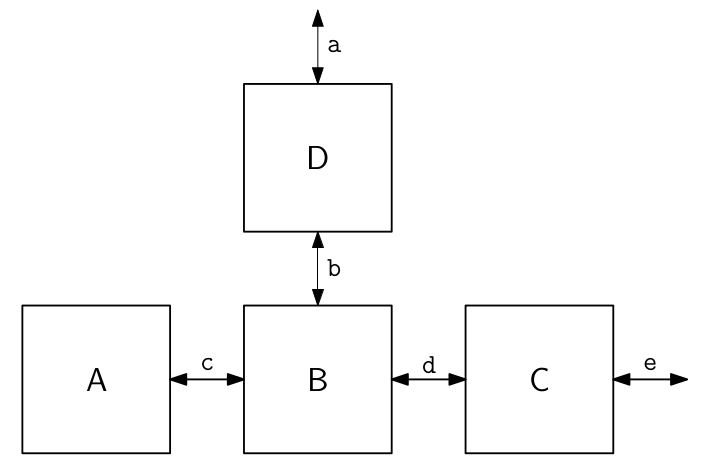
\includegraphics[width=.9\linewidth]{Introduction (Chapter 1)/screenshot_2018-08-25_17-09-03.png}
\end{center}
\#+CAPTION Figure 1.1 An interactive agent A with a port c; An IA B with ports c and d; An IA C with ports d and e; And an IA D with ports b and a. Together they make up an interactive system with open ports a and e When an IA is run it will produce a trace, which is just the sequence of messa

\begin{itemize}
\item When an IA is run it will produce a \texttt{trace}
\begin{itemize}
\item Is a sequence of messages exchanged between the agents in order
\end{itemize}

\item Formally start with the empty trace
\begin{itemize}
\item When \(m\) is written on port \(p\) you append \((\text{SEND},p,m)\) to the trace
\item When \(m\) is read on port \(p\) you append \((\text{READ}, p, m)\) to the trace
\end{itemize}

\item Specification in the book is done via \textbf{trace properties} which are just functions \(P\) which takes traces as input ad return true or false.
\begin{itemize}
\item If \(\tau\) is a trace, then \(P(\tau) = \top\) means that the trace has the property \(P\)
\item \(P(\tau) = \bot\) means that the trace does not have the property \(P\)
\end{itemize}

\item There are two important classes of trace properties
\begin{itemize}
\item \textbf{Safety property:} It is something which is true until some safety condition is broken at which point it never becomes true again	
\begin{itemize}
\item Formally a safety property is a trace property \(P\) suchs that \(P(\epsilon) = \top\) and if \(P(\tau) = \bot\) then \(P(\tau \circ \tau') = \bot\) for all traces \(\tau'\)
\end{itemize}
\item \textbf{Liveness property:} It is something which will eventually become true in some attack model
\begin{itemize}
\item Formally a safety property is a trace property \(P\) suchs that \(P(\epsilon) = \bot\) and if \(P(\tau) = \top\) then \(P(\tau \circ \tau') = \top\) for all traces \(\tau'\)
\end{itemize}
\end{itemize}

\item All traces properties can be written as a conjunction of safety and liveness properties
\end{itemize}

\subsubsection{Types of Distributed Systems Models}
\label{sec:org3c41fcf}
\begin{itemize}
\item \textbf{Fully synchronous:} Each process \(P\) has a clock \(c(P)\) and there is a known bound \(\Delta_\text{CLOCK}\) on how far they drift from real time.
\begin{itemize}
\item There is also a known upper bound \(\Delta_\text{SEND}\) on how long it takes to send a message between any two parties
\item The model often assumes some noting of global time what is used to define what the real time is.
\item \(N\) is used to denote nature and \(c(N)\) to denote real time: the time of nature
\item Hard to implement - almost impossible
\item Easy to use
\end{itemize}

\item \textbf{Fully asynchronous:} The process \(P\) do not even have clocks
\begin{itemize}
\item The protocols cannot be specified b asking parties to do things at specific times
\item There are no know upper bound on how long it takes to send a message
\item It is assumed that if a message is sent by a correct process and that process never crashes
\item The delivery is model as follows
\begin{itemize}
\item There is a value \(\Delta_\text{SEND}\)
\item If a message is send by a correct process that does not crash then it is delivered within that bound
\end{itemize}
\item Easy to implement - almost impossible
\item Hard to use
\end{itemize}

\item \textbf{Eventually synchronous:} A popular mixed model, where the processors have clocks.
\begin{itemize}
\item Two bounds \(\Delta_\text{CLOCK}\) and \(\Delta_\text{SEND}\) are given
\item The clocks can be far apart and messages take arbitrarily long to deliver
\item However, it is assumed that eventually there will always come a period where the network is synchronous
\item Medium to implement
\item Medium to use
\item The goals
\begin{itemize}
\item The safety properties are guarantees always
\item The liveness properties are guaranteed when synchronous
\end{itemize}
\end{itemize}
\end{itemize}

\subsubsection{Canonical Goals}
\label{sec:org56cae34}
\begin{itemize}
\item \textbf{Leader Election:} In many distributed systems, one can gain efficiency by having one server take on a special role, like collecting and distributing tasks.
\begin{itemize}
\item Such a server is often called the leader.
\item The problem is that when the leader crashes, liveness typically breaks down in a very bad way. 
\begin{itemize}
\item Then it is time to pick a new leader.
\item This is called leader election.
\item The goal is that all processes end up agreeing on some new non-crashed process that will be the new leader.
\end{itemize}
\end{itemize}

\item \textbf{Broadcast:} You want to send a message \(m\) to all machines in the system.
\begin{itemize}
\item This is easy when there are no failures.
\item If there are transmission errors, various systems with acknowledgements and resends will solve the problem.
\item In case of process failures, the problem becomes much harder.
\begin{itemize}
\item It is typically needed that all processes receive the same message, even if the sender and some of the other processes crash or are suffering Byzantine failure.
\item The problem can be made even harder by considering many messages being sent by different parties at the same time and require that they arrive in the same order on all processk
\end{itemize}
\end{itemize}

\item \textbf{Consensus:} All processes have a local input bit 0 or 1.
\begin{itemize}
\item This could for instance be a bit indicating whether they are all ready to proceed in the protocol.
\item They should end up outputting a common decision, i.e., there is a bit \(b\) such that all correct processes eventually output \(b\).
\item There are several variations on how this output depends on the inputs.
\end{itemize}

\item \textbf{MUTEX:} Mutual exclusion. The processes run the same code.
\begin{itemize}
\item There is some critical region in the code that only one server is allowed to enter at a time.
\item This problem is already hard in multi-threaded programs.
\item In becomes much worse in a distributed system where the processes are physically separated.
\end{itemize}
\end{itemize}

\section{Communication (2)}
\label{sec:org430c2e7}
\subsection{Types of communication}
\label{sec:org6baa6d2}
\begin{itemize}
\item \textbf{Message Passing:} Processes can send messages to each other
\begin{itemize}
\item The transfer is typically between two parjjjjjjjties only (the sender and receiver)
\item Sending and receiving are separated in time
\end{itemize}

\item \textbf{Shared Memory Space:} Processes are in a setting where they can see the same variables
\begin{itemize}
\item They communicate by writing and reading these variables
\item Different cores and threads on the same computer communicate via this
\end{itemize}
\end{itemize}

\subsection{Lets Go!}
\label{sec:org63042c9}
\begin{verbatim}
package main 

import ( "fmt" )

// A function declaration: Types after variable names; Multiple return values
func multi(x int, y int) (string, int) {
	return "The answer is", x+y
}

// A class
type Named struct {
	name string // Member of a class
}

// Method on a class
func (nm *Named) PrintName(n int) {
	if n < 0 { panic(-1) } // an "exception"
	for i:=0; i<n; i++ {
		fmt.Print(nm.name + "\n")
	}
}

func main() {
	var i int // Explicit declaration of variable
	i = 21
	// = is used for assignment
	j := 21
	// := declares the variable based on the type of the value
	decr := func() int { // a closure
		j = j-7
		return j
	}
	str, m := multi(i, j)
	defer fmt.Println(str, m) // run after return or a panic
	fmt.Println(decr())
	fmt.Println(decr())
	nm1 := Named{ name: "Jesper" } // value
	nm2 := &Named{} // pointer
	nm1.PrintName(2) // Calling a method
	nm2.PrintName(2) // . does auto-dereference of pointer
	nm2.name = "Claudio" ; nm2.PrintName(2) // RETURN or ; as seper
}
\end{verbatim}
\subsection{The Internet}
\label{sec:org5951895}
\subsubsection{IP}
\label{sec:org5049f7f}
\begin{itemize}
\item A Go program which will display the name and IP address of your machine
\end{itemize}
\begin{verbatim}
package main

import (
	"fmt"
	"net"
	"os"
	"strconv"
)

func main() {
	name, _ := os.Hostname()
	addrs, _ := net.LookupHost(name)
	fmt.Println("Name: " + name)
	for indx, addr := range addrs {
		fmt.Println("Address number " + strconv.Itoa(indx) + ": " + addr)
	}
}
\end{verbatim}

\subsubsection{UDP}
\label{sec:org2e0804a}
\begin{itemize}
\item An UDP Server which receives UDP packages and prints then
\end{itemize}
\begin{verbatim}
package main

import (
	"fmt"
	"net"
)

func main() {
	ServerAddr, _ := net.ResolveUDPAddr("udp", ":10001")
	ServerConn, _ := net.ListenUDP("udp", ServerAddr)
	defer ServerConn.Close()
	buf := make([]byte, 1024)
	for {
		n, addr, err := ServerConn.ReadFromUDP(buf)
		fmt.Println("Received ", string(buf[0:n]), " from ", addr)
		if err != nil {
			fmt.Println("Error: ", err)
		}
	}
}
\end{verbatim}

\begin{itemize}
\item A UDP client sending packages to port 10001 on the local machine
\end{itemize}
\begin{verbatim}
package main

import (
	"net"
	"strconv"
	"time"
)

func main() {
	ServerAddr, _ := net.ResolveUDPAddr("udp", "127.0.0.1:10001")
	LocalAddr, _ := net.ResolveUDPAddr("udp", "127.0.0.1:0")
	conn, _ := net.DialUDP("udp", LocalAddr, ServerAddr)
	defer conn.Close()
	i := 0
	for {
		i++
		msg := strconv.Itoa(i)
		conn.Write([]byte(msg))
		time.Sleep(time.Second * 1)
	}
}
\end{verbatim}

\subsubsection{TCP}
\label{sec:orgb82259b}
\begin{itemize}
\item A TCP Server
\end{itemize}
\begin{verbatim}
package main

import ( "net" ; "fmt" ; "bufio" ; "strings" )

func handleConnection(conn net.Conn) {
	defer conn.Close()
	for {
		msg, err := bufio.NewReader(conn).ReadString('\n')
		if (err != nil) {
			fmt.Println("Error: " + err.Error())
			return
		} else {
			fmt.Print("From Client:", string(msg))
			titlemsg := strings.Title(msg)
			conn.Write([]byte(titlemsg))
		}
	}
}

func main() {
	fmt.Println("Listening for connection...")
	ln, _ := net.Listen("tcp", ":18081")
	defer ln.Close() // Makes the function ln.Close() run after main terminates
	conn, _ := ln.Accept() 
	fmt.Println("Got a connection...")
	handleConnection(conn)
}
\end{verbatim}

\begin{itemize}
\item A TCP Client
\end{itemize}
\begin{verbatim}
package main

import (
	"bufio"
	"fmt"
	"net"
	"os"
)

var conn net.Conn

func main() {
	conn, _ = net.Dial("tcp", "127.0.0.1:18081")
	defer conn.Close()
	for {
		reader := bufio.NewReader(os.Stdin)
		fmt.Print("> ")
		text, err := reader.ReadString('\n')
		if text == "quit\n" {
			return
		}
		fmt.Fprintf(conn, text)
		msg, err := bufio.NewReader(conn).ReadString('\n')
		if err != nil {
			return
		}
		fmt.Print("From server: " + msg)
	}
}
\end{verbatim}

\begin{itemize}
\item A go program which starts listening on a random port
\end{itemize}
\begin{verbatim}
package main

import (
	"fmt"
	"net"
)

func main() {
	ln, _ := net.Listen("tcp", ":")
	defer ln.Close()
	_, port, _ := net.SplitHostPort(ln.Addr().String())
	fmt.Println("Listening on port " + port)
}
\end{verbatim}

\subsubsection{DNS}
\label{sec:org6e6d020}
\begin{itemize}
\item Look up the IP address of \url{https://www.google.com}
\end{itemize}
\begin{verbatim}
package main

import (
	"fmt"
	"net"
	"strconv"
)

func main() {
	addrs, _ := net.LookupHost("google.com")
	for indx, addr := range addrs {
		fmt.Println("Address number " + strconv.Itoa(indx) + ": " + addr)
	}
}
\end{verbatim}

\begin{itemize}
\item Ask Google a question
\end{itemize}
\begin{verbatim}
package main

import (
	"bufio"
	"fmt"
	"net"
)

func main() {
	addrs, _ := net.LookupHost("www.google.com")
	addr := addrs[0]
	fmt.Println(addr)
	conn, err := net.Dial("tcp", addr+":80")
	if conn != nil {
		defer conn.Close()
	}
	if err != nil {
		panic(0)
	}
	fmt.Fprintf(conn, "GET /search?q=Secure+Distributed+Systems HTTP/1.1\n")
	fmt.Fprintf(conn, "HOST: www.google.com\n")
	fmt.Fprintf(conn, "\n")
	for {
		msg, err := bufio.NewReader(conn).ReadString('\n')
		if err != nil {
			panic(1)
		}
		fmt.Println(msg)
	}
}
\end{verbatim}
\subsection{Concurrency}
\label{sec:org2f89eab}
\begin{itemize}
\item To coordinate concurrent threads in Go, two abstractions is used MUTEX and channels
\begin{itemize}
\item MUTEX has the type \texttt{Mutex} and has two methods \texttt{Mutex.Lock()} and \texttt{Mutex.Unlock()}
\begin{itemize}
\item Can be held by a single writer or multiple readers
\end{itemize}
\item A channel has a type which is the type of objects that can be send over the channel
\begin{itemize}
\item Any goroutine can send on a channel and any goroutine can receive from a channel.
\item It is safe for many goroutines to send and receive at the same time without using MUTEXs.
\item When a  thread sends on a channel it blocks until the message is read
\item The build in map type is not thread safe
\end{itemize}
\end{itemize}

\item A multithreaded TCP server
\end{itemize}
\begin{verbatim}
package main

import (
	"bufio"
	"fmt"
	"net"
	"strings"
)

func handleConnection(conn net.Conn) {
	defer conn.Close()
	myEnd := conn.LocalAddr().String()
	otherEnd := conn.RemoteAddr().String()
	for {
		msg, err := bufio.NewReader(conn).ReadString('\n')
		if err != nil {
			fmt.Println("Ending session with " + otherEnd)
			return
		} else {
			fmt.Print("From " + otherEnd + " to " + myEnd + ": " + string(msg))
			titlemsg := strings.Title(msg)
			conn.Write([]byte(titlemsg))
		}
	}
}

func main() {
	ln, _ := net.Listen("tcp", ":18081")
	defer ln.Close()
	for {
		fmt.Println("Listening for connection...")
		conn, _ := ln.Accept()
		fmt.Println("Got a connection...")
		go handleConnection(conn)
	}
}
\end{verbatim}

\begin{itemize}
\item A use of channels in Go
\end{itemize}
\begin{verbatim}
package main

import (
	"fmt"
	"strconv"
)

var sendernames = [5]string{"Alice", "Bob", "Chloe", "Dennis", "Elisa"}
var receivernames = [5]string{"Frederik", "Gary", "Hailey", "Isabel", "Jesper"}

func send(c chan string, myname string) {
	for i := 0; i < 1000; i++ {
		// you send on a channel using <-
		c <- myname + "#" + strconv.Itoa(i)
	}
}

func receive(c chan string, myname string) {
	i := 0
	for {
		// you also receive from channel using <-
		msg := <-c
		fmt.Println(myname + "#" + strconv.Itoa(i) + " " + msg)
		i++
	}
}

func main() {
	c := make(chan string)
	for i := 0; i < 5; i++ {
		go send(c, sendernames[i])
		go receive(c, receivernames[i])
	}
	// we do one blocking call to avoid that the program terminates
	receive(c, "Kacey")
}
\end{verbatim}

\begin{itemize}
\item A Go program with a race condition
\end{itemize}
\begin{verbatim}
package main

import (
	"fmt"
	"sync"
)

type DNS struct {
	m    map[string]string
	lock sync.RWMutex
}

func (dns *DNS) Set(key string, val string) {
	dns.lock.Lock()
	defer dns.lock.Unlock()
	dns.m[key] = val
}

func (dns *DNS) Get(key string) string {
	dns.lock.RLock()
	defer dns.lock.RUnlock()
	return dns.m[key]
}

func MakeDNS() *DNS {
	dns := new(DNS)
	dns.m = make(map[string]string)
	return dns
}

func GetAndSet(suf string) {
	for i := 0; i < 10; i++ {
		dns.Set("X", dns.Get("X")+suf)
	}
	c <- 0
}

var c = make(chan int)
var dns = MakeDNS()

func main() {
	go GetAndSet("1")
	go GetAndSet("2")
	go GetAndSet("3")
	<-c
	<-c
	<-c // wait for the three goroutine
}
\end{verbatim}

\begin{itemize}
\item A Go program without a race condition (using locks)
\end{itemize}
\begin{verbatim}
package main

import (
	"fmt"
	"sync"
)

type DNS struct {
	m    map[string]string
	lock sync.Mutex
}

func MakeDNS() *DNS {
	dns := new(DNS)
	dns.m = make(map[string]string)
	return dns
}

func (dns *DNS) GetAndSetOnce(suf string) {
	dns.lock.Lock()
	defer dns.lock.Unlock()
	dns.m["X"] = dns.m["X"] + suf
}

func (dns *DNS) GetAndSet(suf string) {
	for i := 0; i < 10; i++ {
		dns.GetAndSetOnce(suf)
	}
	c <- 0
}

var c = make(chan int)

func main() {
	dns := MakeDNS()
	go dns.GetAndSet("1")
	go dns.GetAndSet("2")
	go dns.GetAndSet("3")
	<-c
	<-c
	<-c // wait for the three goroutines to end
	fmt.Println(dns.m["X"])
}
\end{verbatim}

\subsection{Marshalling}
\label{sec:org1e016a2}
\begin{itemize}
\item Go has a serializability system called \texttt{Gob}
\begin{itemize}
\item In go there is a notion that a field of a struct being exported or not
\begin{itemize}
\item If the name of the field starts with a capital letter it is exported
\end{itemize}
\item Only exported fields are send in Gob
\end{itemize}

\item A TCP server using Gob
\end{itemize}
\begin{verbatim}
package main

import (
	"encoding/gob"
	"fmt"
	"io"
	"log"
	"net"
)

type ToSend struct {
	Msg    string // only exported variables are sent, so start the ...
	Number int    // ... name of the fields you want send by a capital letter
}

func handleConnection(conn net.Conn) {
	defer conn.Close()
	msg := &ToSend{}
	dec := gob.NewDecoder(conn)
	for {
		err := dec.Decode(msg)
		if err == io.EOF {
			fmt.Println("Connection closed by " + conn.RemoteAddr().String())
			return
		}
		if err != nil {
			log.Println(err.Error())
			return
		}
		fmt.Println("From "+conn.RemoteAddr().String()+":\n", msg)
	}
}
func main() {
	fmt.Println("Listening for connection...")
	ln, _ := net.Listen("tcp", ":18081")
	defer ln.Close()
	conn, _ := ln.Accept()
	fmt.Println("Got a connection from ", conn.RemoteAddr().String())
	handleConnection(conn)
}
\end{verbatim}

\begin{itemize}
\item A TCP client using Gob
\end{itemize}
\begin{verbatim}
package main

import (
	"bufio"
	"encoding/gob"
	"fmt"
	"net"
	"os"
)

type ToSend struct {
	Msg    string // only exported variables are sent, so start the ...
	Number int    // ... name of the fields you want sent by a capital letter
}

func main() {
	ts := &ToSend{}
	conn, _ := net.Dial("tcp", "127.0.0.1:18081")
	defer conn.Close()
	enc := gob.NewEncoder(conn)
	for i := 0; ; i++ {
		fmt.Print("> ")
		reader := bufio.NewReader(os.Stdin)
		m, err := reader.ReadString('\n')
		if err != nil || m == "quit\n" {
			return
		}
		ts.Msg = m
		ts.Number = i
		enc.Encode(ts)
	}
}
\end{verbatim}

\subsection{Remote Procedure Calls}
\label{sec:org7170774}
\begin{itemize}
\item Also sometimes called RMI in object oriented languages

\item Remote Procedure Calls works as follows:
\begin{enumerate}
\item The parameters are sent over the network to a remote machine
\item The function is run on some remote value is returned
\item The return values are sent over the network to the caller using serialization
\end{enumerate}

\item An RPC server
\end{itemize}
\begin{verbatim}
package main

import (
	"bufio"
	"fmt"
	"log"
	"net"
	"net/rpc"
	"os"
	"time"
)

type PrintAndCount struct {
	x int
}

func (l *PrintAndCount) GetLine(line []byte, cnt *int) error {
	HardTask()
	l.x++
	fmt.Println(string(line))
	*cnt = l.x
	return nil
}
func HardTask() {
	time.Sleep(5 * time.Second)
}
func MakeTCPListener() *net.TCPListener {
	addy, err := net.ResolveTCPAddr("tcp", "0.0.0.0:42587")
	if err != nil {
		log.Fatal(err)
	}
	inbound, err := net.ListenTCP("tcp", addy)
	if err != nil {
		log.Fatal(err)
	}
	return inbound
}
func main() {
	// Register how we receive incoming connections
	go rpc.Accept(MakeTCPListener())
	// Register a PrintAndCount object
	rpc.Register(new(PrintAndCount))
	// Avoid terminating
	fmt.Println("Press any key to terminate server")
	bufio.NewReader(os.Stdin).ReadLine()
}
\end{verbatim}

\begin{itemize}
\item An synchronous RPC client
\end{itemize}
\begin{verbatim}
package main

import (
	"bufio"
	"fmt"
	"log"
	"net/rpc"
	"os"
)

func main() {
	client, err := rpc.Dial("tcp", "localhost:42587")
	if err != nil {
		log.Fatal(err)
	}
	in := bufio.NewReader(os.Stdin)
	for {
		line, _, err := in.ReadLine()
		var reply int
		// Synchronous call
		err = client.Call("PrintAndCount.GetLine", line, &reply)
		if err != nil {
			log.Fatal(err)
		}
		fmt.Println("Strings printed at server: ", reply)
	}
}
\end{verbatim}

\begin{itemize}
\item An asynchronous RPC client
\end{itemize}
\begin{verbatim}
package main

import (
	"bufio"
	"fmt"
	"log"
	"net/rpc"
	"os"
)

func PrintWhenReady(call *rpc.Call) {
	<-call.Done // this channel unblocks when the call returns
	if call.Error != nil {
		log.Fatal(call.Error)
	}
	fmt.Println("Strings printed at server: ", reply)
}

var reply int

func main() {
	client, err := rpc.Dial("tcp", "localhost:42587")
	if err != nil {
		log.Fatal(err)
	}
	in := bufio.NewReader(os.Stdin)
	for {
		line, _, _ := in.ReadLine()
		// Asynchronous call
		call := client.Go("PrintAndCount.GetLine", line, &reply, nil)
		go PrintWhenReady(call) // Handles the reply when ready
		fmt.Println("See, I can still do stuff!")
		fmt.Println("See, I can still do stuff!")
		fmt.Println("OK, I’m bored...")
	}
}
\end{verbatim}

\subsection{Logically Organising Connections}
\label{sec:org7e57b9b}
\begin{itemize}
\item \textbf{Fully Connected:} Let everyone in the system make a connection to every else
\begin{itemize}
\item Often done in smaller systems where a server is replicated
\item Does not scale well because with \(n\) servers the number of connections is in the order \(n^2\)
\end{itemize}

\item \textbf{Client-Server:} There is a single server to which all the clients connect
\begin{itemize}
\item There is a single point of failure
\begin{itemize}
\item If the server crashed, is attacked or is corrupted the security of the system breaks down
\end{itemize}
\end{itemize}

\item \textbf{Client-Replicated Server:} Replicated servers
\begin{itemize}
\item Deals with the single point of attack problem
\item Most common architecture on the internet
\item Opens up a lot of problems with keeping the copies of the replicated server consistent
\end{itemize}

\item \textbf{Edge nodes:} All access is meditated by edge nodes
\begin{itemize}
\item Client contact the nodes which distribute the work load over the replicates
\item Useful of replicated servers
\end{itemize}
\end{itemize}

\subsection{Unstructured Peer-to-Peer}
\label{sec:orga589cc6}
\subsubsection{General}
\label{sec:org4607e58}
\begin{itemize}
\item There are two main kinds of peer-to-peer networks structured and unstructured
\begin{itemize}
\item In structured the connection between nodes are established in a deterministic way
\item In unstructured the connections are formed at random
\end{itemize}

\item A peer-to-peer graph can be used to disseminate messages.
\begin{itemize}
\item If you want to send a message, simply send it to the peers you have chosen.
\item If a node received a message it did not see before then it recursively disseminate it the same way.
\end{itemize}
\end{itemize}

\begin{figure}[htbp]
\centering
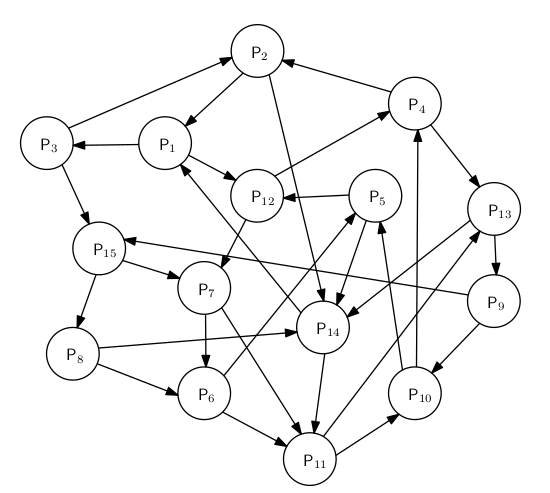
\includegraphics[width=.9\linewidth]{Communication (Chapter 2)/screenshot_2018-08-27_17-18-53.png}
\caption{\label{fig:org90ee680}
Random Peer-to-Peer}
\end{figure}

\begin{itemize}
\item There are two measure of a how good a peer-to-peer graph are
\begin{itemize}
\item \textbf{Diameter:} For each pair \((P_i, P_j)\) of parties, define their distance to be the shortest path from \(P_i\) to \(P_j\). The diameter of the graph is
\end{itemize}
\end{itemize}
\begin{equation} \text{Diameter} = \underset{P_i \ P_j}{max}\ \text{Distance}(P_i, P_j) \end{equation}
\begin{itemize}
\item If they are not connected the distance is \(+\infty\)
\item To compute the distance from two parties one can flood the network starting from \(P_i\) to see how long it takes to reach \(P_j\)
\end{itemize}
\begin{itemize}
\item \textbf{Connectivity:} It is the minimal number of edges that must be removed to make the graph unconnected
\end{itemize}
\begin{itemize}
\item The reason one might use a random peer-to-peer network is that they are easy to form

\item \textbf{THEOREM 2.1} Assume that \(n \geq 25\) and \(\kappa \geq 2\). If you pick a random peer-to-peer graph on \(n\) parties with out degree \(\kappa\), then the probabilty that it is not connected is at most \(2^{-\kappa}\)

\item An \textbf{Eclipsing Attack} is when the adversary controls some nodes \(A \subset P\) and removes the connection and creates a cut 
\begin{itemize}
\item A type of Byzantine Attack
\end{itemize}
\end{itemize}

\subsubsection{How to Build and Maintain}
\label{sec:org7fca6b4}
\begin{itemize}
\item To build a random peer-to-peer network, each node could hold a list of all other nodes present in the network and pick its connections random from this list
\begin{itemize}
\item When a new node enters the network it will flood its presence and all other nodes will add it to their network list
\item If a node becomes unresponsive, nodes will remove it from their network list.
\item To enter the network initially, a node needs to know at least one other node of the network and ask it for its network list.
\end{itemize}

\item In practice it is not possible to have a list of every node on the network, so there are other methods to build a random look network.
\begin{itemize}
\item Each node only holds a partial view.
\item When entering the network you get the partial view of your entry point.
\item Then you can contact some of the know peers to get their partial view and that way learn about more peers, and yourself build a random looking partial view of the system.
\end{itemize}
\end{itemize}

\subsection{Structured Peer-To-Peer}
\label{sec:org0f5757b}
\begin{itemize}
\item A popular structured peer-to-peer network is the Chord network
\begin{itemize}
\item Each node has an identity
\begin{itemize}
\item e.g. IP-address
\end{itemize}
\item The identity is mapped deterministically to an integer between \(0\) and \(B-1\) for some bound \(B\)
\begin{itemize}
\item \(B\) has to large enough so that the change that a node is mapped to the same integer is small
\end{itemize}
\item point as 0, B + 1 would hit the same point as 1 and so on.
\item When a number of nodes with identities \(A, B, C \dots\) enter the network, they will each map their identity into a number.
\item Each node is ordered in a circle
\item Each node will then make a connection the node that is 1 step away on the circle, 2 steps away, 4 steps away8 steps away, 16, 32, and so on.
\item If there is no node at those exact points they make a connection to the next node on the circle.
\item This ensures that the diameter is only \(\log_2(B)\) so that it does not take to long to sent a message
\end{itemize}
\end{itemize}


\begin{center}
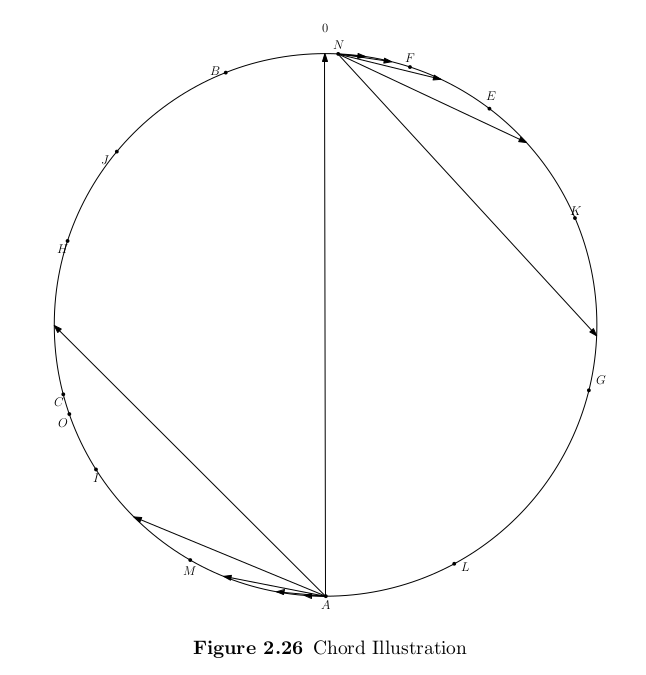
\includegraphics[width=.9\linewidth]{Communication (Chapter 2)/screenshot_2018-08-27_18-25-49.png}
\end{center}

\section{A Syntax for Distributed Systems (3)}
\label{sec:org3ca03b8}
\subsection{Basic System Model}
\label{sec:org721bccf}
\subsubsection{Interactive Agents}
\label{sec:org140f45b}
\begin{itemize}
\item The most basic entity will be an Interactive Agent (IA), which is formally defined by a tuple \((\mathcal P, \sigma_0, T)\) where:
\begin{itemize}
\item \(\mathcal P\) is a finite set containing the ports which the IA can receive inputs and outputs
\begin{itemize}
\item Each ports can be used for both sending and receiving
\end{itemize}
\item \(\sigma_0\) is the initial state of the IA
\item \(T\) is the transition function
\begin{itemize}
\item It says what the system does in response to a message being received on one of the ports
\item Depends on the current state \(\sigma\), the port name \(P \in \mathcal P\) and the message \(m\) being received
\item The output specifies the new current state \(\sigma'\), a new port \(Q \in \mathcal P\) and some new message \(m' \in \mathcal P\)
\begin{itemize}
\item It is written \((\sigma',Q,m') \leftarrow T(\sigma, P, m)\)
\item The transition function always send a new message on some legal port
\end{itemize}
\end{itemize}
\end{itemize}

\item The IA \(A\) is thought of as a box holding its current state \(\sigma\)
\item The syntax \((Q,m') \leftarrow A(P,m)\) is used to mean: fetch the current state \(\sigma\) from \(A\) and compute \((\sigma',Q,m') \leftarrow T(\sigma,P,m)\)  and replace the current state in \(A\) by \(\sigma'\)

\item The transition function is allowed to be randomised
\begin{itemize}
\item This allows to model an algorithm which for instance samples a random RSA key \((n,e,d)\), saves \((n,d)\) in the state \(\sigma'\) and sends \((n,e)\) on some port.
\end{itemize}

\item The transition function should not depend on port names
\begin{itemize}
\item Done to avoid conflicting port names
\end{itemize}
\end{itemize}

\subsubsection{Interactive Systems}
\label{sec:org49229be}
\begin{itemize}
\item An interactive system (IS) \(S\) is a set of IAs
\begin{itemize}
\item If there are two IAs with the same port name, they are thought of as being connected
\item If there are more than two IAs with the same port name the system is \textbf{malformed} and \(S = \bot\) is written
\item Composing two systems \(S_1\) and \(S_2\) is done by taking the set union \(S_1+S_2 = S_1 \cup S_2\)
\end{itemize}

\item The ports not connected to other ports are called \textbf{open ports}
\begin{itemize}
\item An IS can be activated on an open port \(P\) by sending some message \(m\)
\end{itemize}

\item If \((P,m)\) is inputted to \(S\), the execution proceeds as follows
\begin{enumerate}
\item Let \(A_0\) be the IA with port \(P\), let \(m_0 = m\) and \(P_0 = O\), e then compute \((P_1, m_1) \leftarrow A_0(P_0, m_0)\)
\item If \(P_1\) is a closed port, then let \(A_1\) be the other IA with port \(P_1\). We then compute \((P_2, m_2) \leftarrow A_0(P_1, m_1)\) and so on until we compute \((P_{t+1}, m_{t+1}) \leftarrow A_t(P_t, m_t)\) and \(P_{t+1}\) is an open port
\item Then let \(Q = P+1\) and \(m' = m_{t+1}\) return \((Q, m')\)
\end{enumerate}

\item When compute an output the IS also updates its internal state of the system
\begin{itemize}
\item An IS is therefore in some sense just a more structured IA
\end{itemize}
\end{itemize}

\subsection{Modelling Persistent Storage}
\label{sec:orgf18f4fa}
\begin{figure}[htbp]
\centering
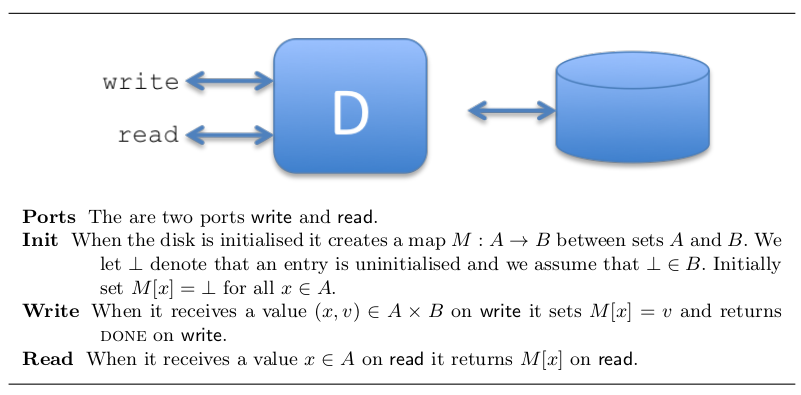
\includegraphics[width=.9\linewidth]{A Syntax for Distributed Systems (3)/screenshot_2018-09-02_11-00-00.png}
\caption{\label{fig:org8a0042d}
A Disk. To the left, the structure of the disk. To the right, how we will depict it in the rest of the text.}
\end{figure}

\begin{itemize}
\item The book gives an oversimplified model of persistent storage
\begin{itemize}
\item Implementing it in practise is a whole science in itself
\item Atomicity is for example hard to implement
\end{itemize}
\end{itemize}

\subsection{Modelling Processes}
\label{sec:org417a0c0}
\subsubsection{General}
\label{sec:orga54da25}
\begin{figure}[htbp]
\centering
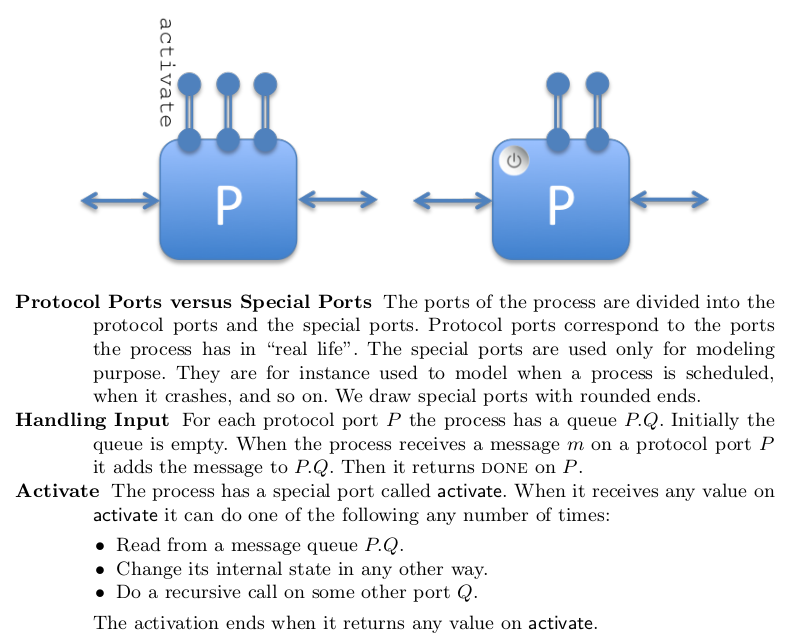
\includegraphics[width=.9\linewidth]{A Syntax for Distributed Systems (3)/screenshot_2018-09-02_11-20-12.png}
\caption{\label{fig:org409bc0a}
A Process. To the left, its structure. To the right, how we depict it in the rest of the text.}
\end{figure}

\begin{itemize}
\item The model of processes given is based solely on message passing and pure asynchronous programming
\begin{itemize}
\item All inputs to a process are given as messages and are queued on the receiving process in such a way that the "calling" process can proceed its execution immediately.
\item The caller never waits on its input
\end{itemize}

\item A process will receive its input asynchronously as follows
\begin{itemize}
\item When a message \(m\) is received on some port \(P\), the message \(m\) is added to queue \(Q\), then process returns and does nothing more
\item There is a separate "thread" associated to the process which does the actual work
\begin{itemize}
\item It proceeds in steps known as activations
\item In each activation it is allowed to do some small amount of work and then the activation stops again
\end{itemize}
\end{itemize}

\item To model that processes by default might not progress at the same speed, a special port is introduced on which the process is told when to do the activations.
\begin{itemize}
\item Think of some evil daemon being connected to these ports.
\item We cannot by default assume that all processes proceed at the same speed, so to be on the safe side we assume that the order in which they take steps could be the worst possible one.
\end{itemize}
\end{itemize}

\subsubsection{Specifying a Process}
\label{sec:org34e11a1}
\begin{itemize}
\item Formally a process is given by a transition function
\begin{itemize}
\item A very cumbersome formalism
\end{itemize}

\item The process is instead specified by a list of activation rules written in prose or pseudo-code, some examples of activation rules:
\begin{itemize}
\item On input \((\text{INCREMENT},a)\) on \(I\), let \(x \leftarrow x+a\) and send \(x\) on port \(P\)
\item On input \((\text{PING})\) on \(P\) return on \(P\)
\item On input \((\text{CONDITIONAL-INCREMENT},a,b,)\), if \(x \leq b\), let \(x \leftarrow x+a\) and send \(x\) on port \(P\)
\end{itemize}

\item In its more general form an activation rule has the format /"On input \((\text{NAME}, v_1, v_2, \dots, )\) on port \(P\), if Cond, do \(A\)"
\begin{itemize}
\item The rule is \texttt{triggerable} if in the queue \(P.Q\) there is a message \(m\) of the form \((\text{NAME}, v_1, v_2, \dots, )\) and at the same time the condition Cond is true
\item The condition might depend on the message and the internal state of the process
\item If the rule is triggered the \(m\) is removed from the queue, if not the message is not removed.
\item If the rule is triggered then the algorithm \(A\) is run
\begin{itemize}
\item This algorithm is allowed to run as a normal activation of a process
\item After running \(A\) the process return on \texttt{activate}
\end{itemize}
\item When a process is activated port \texttt{activate} it goes though all its activation rules from top to bottom
\begin{itemize}
\item If it finds on which is triggerable it triggers that rule
\item If no activation rule is triggerable it does nothing and returns immediately on \texttt{activate}
\item If no activation rule is triggerable we say the process is \texttt{idle}
\end{itemize}
\end{itemize}
\end{itemize}

\subsubsection{Some Possible Special Ports}
\label{sec:org5025cb9}
\begin{itemize}
\item In addition to \texttt{activate} a process might have other special ports.
\begin{itemize}
\item These special ports are typically used to model faults.
\end{itemize}

\item Examples of special ports.
\begin{itemize}
\item \textbf{crash:} On any input on the crash port, delete the process’ set of activation rules.
\begin{itemize}
\item This means that the machine no longer does anything when activated.
\end{itemize}
\item \textbf{takeover:} On input \texttt{AR} on takeover the activation rules of the process are replaced by the activation rules in AR.
\begin{itemize}
\item If the process models a machine, then this corresponds to a hacker completely taking over the machine and installing its own code on the machine.
\end{itemize}
\item \textbf{leak:} On input \(L\) on leak, let \(\sigma\) denote the internal state of the process, including all the queues of incoming messages. Compute \(y=L(\sigma)\). Then return \(y\) on leak.
\begin{itemize}
\item This corresponds to the process leaking some information to its environment.
\item If the leakage function L is the identity, then it corresponds to a hacker breaking into the machine and seeing all the data on the machine.
\item In some case more limited leakage makes sense too.
\end{itemize}
\end{itemize}

\item By default a process only has the \texttt{activate} special port
\end{itemize}

\subsection{Modelling Cnhannels}
\label{sec:org1269d63}
\begin{figure}[htbp]
\centering
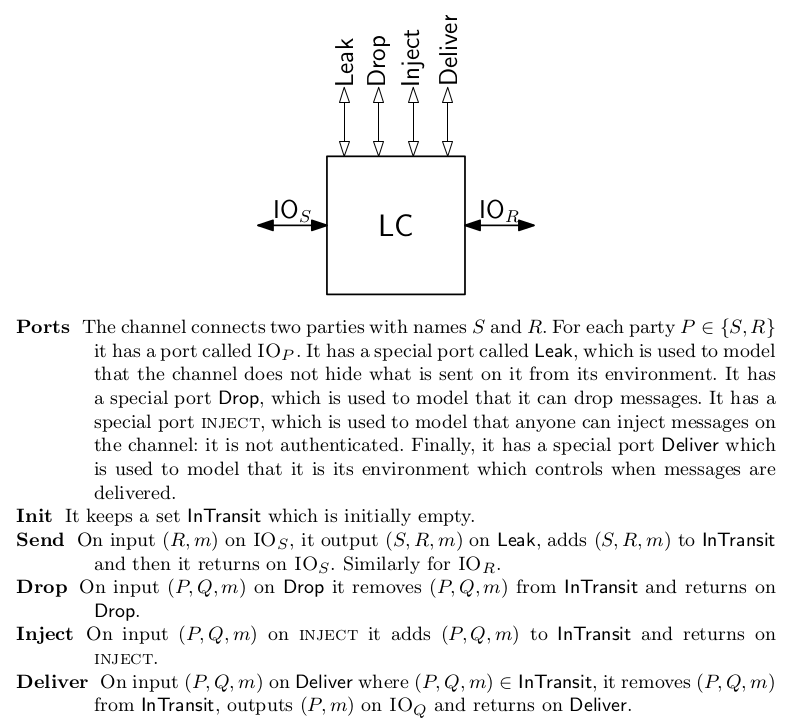
\includegraphics[width=.9\linewidth]{A Syntax for Distributed Systems (3)/screenshot_2018-09-02_11-51-41.png}
\caption{\label{fig:orge40e5dd}
Lossy Channel}
\end{figure}


\begin{figure}[htbp]
\centering
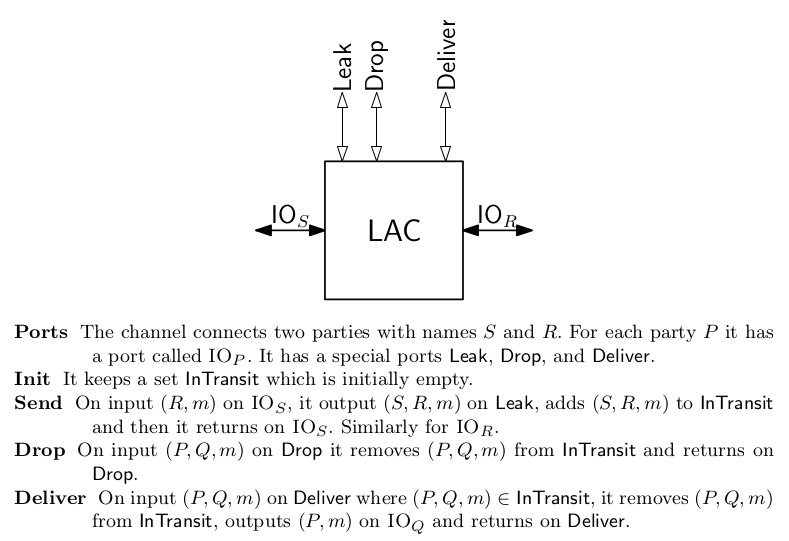
\includegraphics[width=.9\linewidth]{A Syntax for Distributed Systems (3)/screenshot_2018-09-02_12-03-24.png}
\caption{\label{fig:org2133f9c}
Lossy Authenticated Channel}
\end{figure}


\begin{figure}[htbp]
\centering
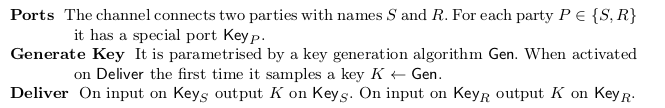
\includegraphics[width=.9\linewidth]{A Syntax for Distributed Systems (3)/screenshot_2018-09-02_12-09-02.png}
\caption{\label{fig:org2ba306d}
KDC}
\end{figure}


\begin{itemize}
\item The same distinction between protocol ports and special ports is used
\end{itemize}

\subsection{Modelling Protocols}
\label{sec:orgbd79b4e}
\begin{center}
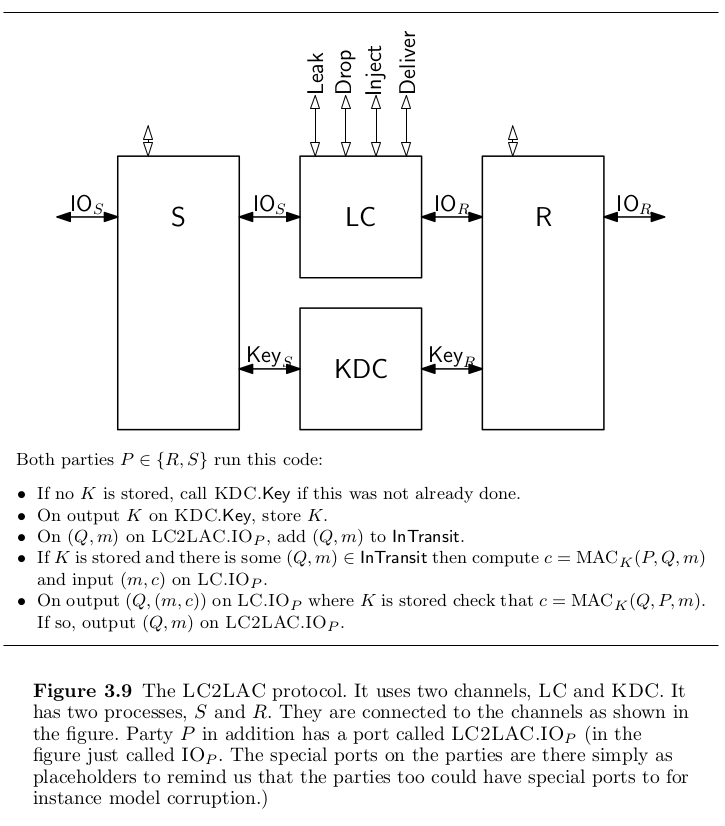
\includegraphics[width=.9\linewidth]{A Syntax for Distributed Systems (3)/screenshot_2018-09-02_12-17-35.png}
\end{center}
\begin{itemize}
\item Protocols wil consist of processes, channels and disks connected to to each other in some way
\end{itemize}

\subsection{Specifying Safety Properties}
\label{sec:org1606852}
\begin{itemize}
\item Safety properties asically specify what is the correct relation between the inputs and the outputs of the system
\begin{itemize}
\item A safety property is only broken if the system gives a wrong output
\end{itemize}

\item \textbf{Definition 3.1 (Security):} We say that a protocols \(\pi\) securely implements a channel \(C\) if there exists an interactive agent Sim that connects only to the special ports of \(C\) and such that \(\pi\) and \(C+\text{Sim}\) have the same input output behavior. We write \(\pi \sqsubseteq C\)
\end{itemize}

\subsection{Specifying Liveness Properties}
\label{sec:orga8cfc85}
\begin{itemize}
\item Liveness properties specify that the system must make progress
\begin{itemize}
\item e.g. that there are no deadlocks
\item A liveness property is only broken if the system ends up in a state where there is still work to do but the state of the system prevents it from making progress again
\end{itemize}
\end{itemize}

\subsection{Composition}
\label{sec:orgb6d9e1b}
\begin{itemize}
\item Composability is an essential property of any definition of security.
\begin{itemize}
\item If composability holds in the model, then we can prove the properties of the combined protocol in a modular way.
\item This allows us to given a simpler and modular analysis where each step focuses only on one small part of the system (for instance, turning a lossy channel into a non-lossy channel).
\end{itemize}
\end{itemize}

\section{Consistent Communication (4)}
\label{sec:orga70dfb3}
\subsection{General}
\label{sec:orgbbf9d57}
\begin{itemize}
\item In many types of networks message can overtake each other
\begin{itemize}
\item This means that you might receive a message \(A\) which depends on another message \(B\) before you receive \(V\)
\item It might also be you don't receive messages from \(P_1\) in the order which they where send by \(P_1\)
\end{itemize}

\item It is assumed that there is access to a flooding system
\begin{itemize}
\item It guarantees that if a correct party sends a message then it is eventually delivered at all correct processes
\end{itemize}

\item A system with the following syntax is considered, indicating how a distributed system interacts with the rest of the worlds
\begin{itemize}
\item \textbf{Send:} A party \(P_i\) can get input on the for \((P_i,m)\).
\item We say that \(P_i\) sent \(m\)
\item A correct process will physically send a message as soon and it gets it as input
\item \textbf{Deliver} A party \(P_i\) can give output of the form \((P_j,m)\) for \(P_j \ne P_i\).
\item We say that the message \(m\) sent by \(P_j\) was delivered by \(P_i\), which is \emph{not} the same event as when the message physically arrives at \(P_i\)
\end{itemize}

\item It is assumed that all messages sent by a given party \(P_i\) are distinct such that \((P_i,n)\) uniquely identifies a \emph{"sent event"}
\item It is assumed that all messages are immediatly delivered local

\item It is assumed that the network start from the following property
\begin{itemize}
\item \textbf{Liveness} If a correct \(P_i\) send \((P_i,m)\), then eventually all correct \(P_j\) deliver \((P_i,m)\)
\end{itemize}
\end{itemize}
\subsection{First In, First Out}
\label{sec:org709bf58}
\begin{itemize}
\item \textbf{FIFO:} If a correct \(P_i\) sends \((P_i,m)\) and later sends \((P_i,m')\), then it holds for all correct \(P_j\) that if they deliver \((P_i,m')\) then they delivered \((P_i,m)\) earlier

\item The following protocol is considered
\begin{enumerate}
\item Initially each party \(P_i\) will initialize a counter \(c_i = 0\).
\begin{itemize}
\item This counter keeps track of how many messages the party \(P_i\) has already sent.
\item Each party \(P_i\) also initializes \(n\) counters \(r_{i,j}=0\) for \(j=0,\dots,n\)
\begin{itemize}
\item These counters keep track of how many messages party \(P_i\) has received from party \(P_j\).
\end{itemize}
\end{itemize}
\item \(P_i\): When sending a message \(x\), send \((P_i,c_i,x)\) on the flooding network and let \(c_i = c_{i + 1}\).
\begin{itemize}
\item This mean that we tag each message with how many messages were sent before it.
\end{itemize}
\item \(P_i\): When receiving \((P_j,c_j,x)\) store it in a buffer until \(r_{i,j} = c_j\). Then let
\end{enumerate}
\end{itemize}
\(r_{i,j}=r_{i,j+1}\) and output \((P_j,m)\).

\begin{itemize}
\item If all parties are correct the FIFO protocol ensures that all messages from each \(P_i\) are delivered by all other parties in the order they where send by \(P_i\)
\end{itemize}

\subsection{Causality}
\label{sec:org4b75947}
\subsubsection{The Causal-Past Relation}
\label{sec:orga02f70f}
\begin{itemize}
\item The Causal-Past Relation is a binary relation \(\hookrightarrow\) on messages \((P,m)\)
\begin{itemize}
\item It is written as \((P_i,m_i) \hookrightarrow (P_j,m_j)\)
\item It means that in a particular run on the system \(m_j\) might depend on \(m_i\)
\item e.g. because \(P_j\) received \(m_i\) before it sent \(m_j\)
\item Note that the fact that \(P_j\) received \(m_i\) before sending \(m_j\) does not necessarily mean that \(m_j\) in fact depends on \(m_i\) , only that it might depend on \(m_i\).
\item Not all sent events are a Causal-Past Relation
\end{itemize}

\item \(\text{CausalPast}(P_j,m_j)\) is used to denote the set of \((P_i,m_i)\) on which \((P_j,m_j)\) may depend i.e.
\end{itemize}
\begin{equation}
    \text{CasualPast}(P_j,m_j) = \{ (P_i,m_i) | (P_i,m_i) \hookrightarrow (P_j, m_j)\}
\end{equation}

\begin{itemize}
\item Method that keeps track of auxiliary sets \(\text{CausalPast}(P_i)\)
\begin{enumerate}
\item Initially let \(\text{CausalPast}(P_i) = \emptyset\) for all \(P_i\)
\item On input \((P_i,m)\) at \(P_i\), let \(\text{CausalPast}(P_i) = \text{CausalPast}(P_i) \cup \{(P_i,m)\}\) and let \(\text{CausalPast}(P_i,m)=\text{CausalPast}(P_i)\)
\item On output \((P_j,m)\) at \(P_i\), let \(\text{CausalPast}(P_i) = \text{CausalPast}(P_i) \cup \text{CausalPast}(P_j,m)\)
\end{enumerate}
\end{itemize}


\begin{itemize}
\item \(\hookrightarrow\) has the following properties
\begin{itemize}
\item \textbf{Transitive:} If \((P_i, m_i) \hookrightarrow (P_j,m_j)\) and \((P_j, m_j) \hookrightarrow (P_k,m_k)\) then \((P_i, m_i) \hookrightarrow (P_k,m_k)\)
\item \textbf{Reflective:} For all messages it holds that \((P_i, m_i) \hookrightarrow (P_i,m_i)\)
\item \textbf{Antisymmetric:} If \((P_i, m_i) \hookrightarrow (P_j,m_j)\) and \((P_j, m_j) \hookrightarrow (P_i,m_i)\) then \((P_i, m_i) = (P_j,m_j)\)
\end{itemize}
\end{itemize}

\subsubsection{A Protocol for Causally Consistent Communication}
\label{sec:org5fcbbee}
\begin{itemize}
\item The safety property of causal order flooding
\begin{itemize}
\item \textbf{Causal Consistency:} If \((P_i,m) \hookrightarrow (P_j,m')\) then it holds for all correct \(P_k\) that if they deliver \((P_j,m')\), then they have previously delivered \((P_i,m)\)
\end{itemize}

\item A very inefficient but trivially safe protocol with has the safety property of causal order flooding 
\begin{enumerate}
\item Initially let \(\text{CausalPast}(P_i) = \emptyset\) for all \(P_i\) and let \(\text{Delivered}(P_i) = \emptyset\)
\item On input \((P_i,m)\) at \(P_i\), let \(\text{CausalPast}(P_i)= \text{CausalPast}(P_i) \cup \{(P_i,m) \}\) and let \(\text{CausalPast}(P_i,m)=\text{CausalPast}(P_i)}\). Then send \((P_i, m)\) and send along \(\text{CausalPast}(P_i,m)\)
\item On receiving \((P_j,m)\) at \(P_i\) along with \(\text{CausalPast}(P_j,m)\) wait until \(\text{CausalPast}(P_j,m) \subseteq \text{Delivered}(Pi) \cup \{ (P_j,m) \}\). Then deliver \((P_j,m)\) and let \(\text{CausalPast}(P_i) = \text{CausalPast}(P_i) \cup \text{CausalPast}(P_j,m)\). Also add \((P_j,m)\) to \(\text{Delivered}(P_i)\)
\end{enumerate}
\end{itemize}

\subsubsection{Vector Clocks}
\label{sec:org7dfe0a4}
\begin{itemize}
\item Vector clocks improve trivial safety protocol

\item Instead of maintaining his causal past each \(P_i\) maintains an array \(\text{VectorClock}(P_i)\) of integers
\begin{itemize}
\item \(\text{VectorClock}(P_i)[P_k]\) is the number of messages that have currently been received from \(P_k\)
\item When a message \(m_i\), \(P_i\) will append the current state of his vector clock to the message
\begin{itemize}
\item Denoted \(\text{VectorClock}(P_i,m_i)\)
\end{itemize}
\item \(\text{VectorClock}(P_i,m_i)[P_k]\) is the number of messages \(P_i\) has received from \(P_k\)  at the time he sent \(m_i\)
\end{itemize}

\item Instead of remembering all message that were delivered each \(P_i\) will maintain an array \(\text{Delivered}(P_i)\) of the same time as vector clocks
\begin{itemize}
\item Where \(\text{Delivered}(P_i)[P_k]\) contains the number of messages from \(P_k\) that were delivered
\end{itemize}

\item For two vector clocks \(\text{VectorClock}(P_i,m_i)\) and \(\text{VectorClock}(P_j,m_j)\) we define
\end{itemize}
\begin{equation}
  \text{VectorClock}(P_i,m_i) \leq \text{VectorClock}(P_j,m_j)
\end{equation}
to mean that
\begin{equation}
  \forall P_k (\text{VectorClock}(P_i,m_i)[P_k] \leq \text{VectorClock}(P_j,m_j))[P_k]
\end{equation}

\begin{itemize}
\item Vector clocks are not always comparable  and we can also compare a vector clock to a Delivered-array. We define
\end{itemize}
\begin{equation}
	\text{VectorClock} = \max(\text{VectorClock}(P_i,m_i), \text{VectorClock}(P_j,m_j))
\end{equation}
to mean that
\begin{equation}
    \forall P_k (\text{VectorClock}[P_k] = \max(\text{VectorClock}(P_j,m_j)[P_k], \text{VectorClock}(P_i,m_i)[P_k]))
\end{equation}

\begin{itemize}
\item For at vector clock \(\text{VectorClock}\) let \(\text{VectorClock}+P_j\) be the same vector clock but where 1 is added to the position \(\text{VectorClock}[P_j]\)

\item The following is a vector clock based protocol for consistent communication
\begin{enumerate}
\item \(P_i\): Initially let \(\text{VectorClock}(P_i)[P_j] = 0\) and let \(\text{Delivered}(P_i)[P_j]\)  for all \(P_j\)
\item On input \((P_i,m)\) at \(P_i\)
\begin{enumerate}
\item Let \(\text{VectorClock}(P_i)[P_i] = \text{VectorClock}(P_i)[P_i] +1\)
\item Let \(\text{VectorClock}(P_i,m)=\text{VectorClock}(P_i)\)
\item Send \((P_i,m)\) along \text{VectorClock}(P\(_{\text{i,m}}\))
\end{enumerate}
\item On receiving \((P_j,m)\) at \(P_i\) along with \(\text{VectorClock}(P_j,m)\)
\begin{enumerate}
\item Wait until .\(\text{VectorClock}(P_j,m) \leq \text{Delivered} (P_i) + P_j\).
\item Then deliver \((P_j,m)\)
\item Let \(\text{VectorClock}(P_i) = \max(\text{VectorClock}(P_i,m_i), \text{VectorClock}(P_j,m_j))\)
\item Increment \(\text{Delivered}(P_i)[P_j]\) by \(1\)
\end{enumerate}
\end{enumerate}
\end{itemize}

\subsection{Total Order}
\label{sec:orga931433}
\begin{itemize}
\item \textbf{Total Order:} If a correct \(P_k\) delivered \((P_i,m)\) and then later delivered \((P_j,m')\) then it holds for all correct \(P_m\) that if they deliver \((P_k,m')\), then they earlier delivered \((P_i,m)\)
\begin{itemize}
\item To ensure total order you can use the casual order system and ping all other machines an wait for an ack for all other machines, this ensures that there are no
\end{itemize}
\end{itemize}

\section{Confidentiality (5)}
\label{sec:org3d54c54}
\subsection{Confidentiality, Secret-Key Systems}
\label{sec:org10dd29e}
\subsubsection{General}
\label{sec:orgbb9ebe2}
\begin{itemize}
\item A secret-key cryptosystem consists of three algorithms
\begin{itemize}
\item One for generating a key: \(G\)
\item One for encryption: \(E\)
\item One for decryption: \(D\)
\end{itemize}

\item The algorithm \(G\) typically generates a key by outputting a randomly chosen bit stïrng of a fixed length
\item The algorithm \(E\) takes as input a key \(k\) and a message \(m\) and outputs a \textbf{ciphertext} \(c\)
\item The algorithm \(D\) takes a ciphertext \(c\) and a key \(k\) and produces a plaintext \(D_k(c)\)
\item It must hold that
\end{itemize}
\begin{equation}
  m=D_k(E_k(m))
\end{equation}

\begin{itemize}
\item The system should makes sure that when an adversary sees \(c\) but not \(k\) it should have no idea whatsoever what it represents
\end{itemize}

\subsubsection{The One-time Pad and Perfect Secrecy}
\label{sec:orgd506e21}
\begin{itemize}
\item If each encryption key is only used once, it is not too difficult to design an unbreakable encryption algorithm, which takes the form of the so-called onetime pad.
\begin{itemize}
\item A one-time pad is quite useless in practice
\end{itemize}
\end{itemize}


\begin{itemize}
\item The \textbf{one-time pad} is constructed as follows 
\begin{itemize}
\item Assuming the message is a string of bits labeled \(m_1, \dots,m_t\)
\item The key will by a random bit sting of the same length as the message labeled \(k_1, \dots, k_t\)
\item Encryption is done by taking the bit-wise xor of the strings
\begin{itemize}
\item The ciphertext \(c_1, \dots, c_t\) is defined by \(c_i = m_i \oplus k_i\)
\end{itemize}
\item The receiver who knows the same key can recover the plaintext by decrypting each i'th bit as
\end{itemize}
\end{itemize}
\begin{equation}
  c_i \oplus k_i  = m_i
\end{equation}

\begin{itemize}
\item \textbf{Theorem 5.1} When one-time pad is used for encryption the ciphertext is always a uniformly distributed bit string, in particular, it is independent of the plaintext.

\item It is said that a cryptosystem has \textbf{perfect secrecy} when the cipher text is independent of the plaintext 
\begin{itemize}
\item This holds no matter how much computing power the eavesdropper has
\end{itemize}

\item \textbf{Theorem 5.2} Suppose a cryptosystem can handle \(\mathcal M\) possible plaintexts, and uses \(\mathcal C\) ciphertexts and \(\mathcal K\) keys. If the system has perfect secrecy, then it must be the case that \(K \geq C \geq M\)
\end{itemize}

\subsubsection{Practical systems, Definition of Security}
\label{sec:orgffa9e62}
\begin{itemize}
\item In practical systems one typically have to settle for computational security
\begin{itemize}
\item One would have to spend unrealistically amount of time to break the system
\end{itemize}

\item Computational security  has several consequences for how we should design cryptosystems and use them
\begin{itemize}
\item The adversary should have no idea what we are sending even if we use the system several times,
\end{itemize}
\end{itemize}


\begin{itemize}
\item Good encryption algorithms work not only with the input \(k\), \(m\) as input, they also make a choice of some variable who value changes from one encryption operation to the next
\begin{itemize}
\item Is called a \textbf{nonce}
\item It must chosen in some way such that we will not use the same value twice
\item It can take the form of a counter or random bits
\item This makes sure that if we encrypt the same message twice it will have different cipher texts
\item To emphasize that a nonce \(n\) was used in the encryption process we write
\end{itemize}
\end{itemize}
\begin{equation}
  c = E_k(m,n)
\end{equation}

\begin{itemize}
\item \textbf{Definition 5.3} Consider any adversary who plays the above game and whose computing power is limited in the sense that whatever algorithm he runs terminates in time much less than the time it takes to try all possible keys in the cryptosystem. No such adversary can guess whether he is in case 1) or 2) (with probability better than essentially a random guess). Cases where m is a message and \(r\) is a random message the same length as \(m\)
\begin{enumerate}
\item \(C=E_k(m,n)\)
\item \(E_k(r,n)\)
\end{enumerate}
\end{itemize}

\subsubsection{Exhaustive Search}
\label{sec:orgb3595c4}
\begin{itemize}
\item A consequence of reusing the same many times is that a system can only be secure if the adversary's resources are limited
\begin{itemize}
\item We have to assume that an adversary does not have enough computing power to run through all possibilities for the key \(k\)
\end{itemize}

\item If the hacker finds out one or more plaintext(s) \(m\) corresponding to a ciphertext(s) \(c\). It means he can execute the simple algorithm \textbf{exhaustive key search}:
\begin{enumerate}
\item Initialize an empty list \(L\)
\item For every possible key \(k'\): compute \(D_k'(c)\) and check if \(D_k'(c)=m\) for all the plaintext/ciphertext pairs \((m,c)\) that are known
\begin{itemize}
\item If this is the case add \(k'\) to the list \(L\)
\end{itemize}
\end{enumerate}

\item \textbf{Fact:} If the adversary knows \(u\) bits of the plaintext (and matching ciphertext), and \(u\) is larger that the length of the key, then we can expect that exhaustive search will identify the correct key.

\item To make sure that exhaustive search is infeasible, a secure system these days must use keys of length about \(128\) bits or more – since doing \(2^{128}\) repetitions of some non-trivial computation is currently considered completely infeasible.
\begin{itemize}
\item Key length by itself is no guarantee for security it is only a necessary condition, because given \(m,c\) there might be a much faster way to find the key than to try all possibilities
\end{itemize}

\item Thinking in terms of exhaustive search is part of estimating the \texttt{cost of an attack} and balancing that with the \texttt{probability of an attack}.
\begin{enumerate}
\item Say that if someone breaks your system you will lose \(C\) dollars
\item There is a probability \(p\) that an attacker can break into the system
\item Then the expected cost of attacks on the system is \(pC\) dollars.
\begin{itemize}
\item You in general want the amount \(pC\) to be negligible i.e. something you don't mind paying
\end{itemize}
\end{enumerate}
\end{itemize}

\subsubsection{Stream Ciphers}
\label{sec:orgd8b4cfc}
\begin{itemize}
\item A steam cipher is an algorithm \(G\) that expands a short key \(k\) and a nonce \(n\) to a much longer random looking string \(G(k,n)\) which is then used to encrypt the message as if it was a onetime pad
\begin{itemize}
\item The receiver must know not only \(k\) but also \(n\) to decrypt the message,
\item \(n\) is not secret so it can just be send along the ciphertext
\end{itemize}

\item A stream cipher in practise does not generate the entire output at once and it does not know the length in advance
\begin{itemize}
\item It fits nicely with application where the input to be encrypted arrives as a stream e.g. byte by byte
\begin{itemize}
\item e.g. a user typing on a keyboard
\end{itemize}
\end{itemize}

\item A well known example of a stream cipher is RC4 which is often used in web browsers, which is rather unfortunate as it has some known weaknesses and should not be used.
\begin{itemize}
\item However, in recent years other, more and very fast secure streamciphers have been proposed such as \texttt{SALTA20} and \texttt{SNOW}
\end{itemize}
\end{itemize}

\subsubsection{Block Ciphers}
\label{sec:orga9925f4}
\begin{itemize}
\item Block ciphers encrypt in their basic form a fixed size block of data, and output a block of the same size as the input.
\begin{itemize}
\item Examples are the former US standards DES (56 bit keys, 64 bit blocks), triple-DES (112 bit keys, 64 bit blocks) and the present standard AES (128 bit keys and blocks).
\end{itemize}

\item To use a block cipher in practice, one needs so called Modes of Operation
\begin{itemize}
\item Which are general methods that allow using a block cipher to encrypt a string of data of any length, and also to achieve security as required in Definition 5.3.
\item Examples are Cipher Block Chaining (CBC) mode, Counter (CTR) Mode, and Output Feedback (OFB) mode.
\item The modes need as input not only the key and the message, but also a nonce
\begin{itemize}
\item In modes-of-operation lingo the nonce if called an \textbf{initialization vector}, \(IV\)
\end{itemize}
\end{itemize}

\item \textbf{OFB mode} is a mode that can be used to make a block cipher function in a way similar to a stream
\begin{itemize}
\item The output is computed by feeding the output block back into the encryption function
\item It creates a seemingly random stream of bits as needed for a stream cipher
\end{itemize}

\item A commonly used mode is \textbf{CBC mode}
\begin{itemize}
\item Assume the message consists of 128 bit block \(M_1, \dots, M_t\) where we pad the last block \(i\) in some way if it does not fill the required block length
\item Then the cipher text will be \(t+1\) blocks \(C_0, \dots, C_t\), where \(C_0=IV\) and for \(i=1, \dots, t\)
\end{itemize}
\end{itemize}
\begin{equation}
  C_i = AES_K(M_i \oplus C_{i-1})
\end{equation}

\begin{itemize}
\item \textbf{CTR mode}
\begin{itemize}
\item The message consists of 128 bit block \(M_1, \dots, M_t\) as in CBC mode and the cipher text depends on an \(IV\)
\item The ciphertext will be \(t+1\) block \(C_0, \dots, C_t\) where \(C_0=IV\) and for \(i=1, \dots, t\)
\end{itemize}
\end{itemize}
\begin{equation}
  C_i=AES_k(IV+i) \oplus M_i
\end{equation}
\begin{itemize}
\item \(IV+i\) means think of \(IV\) as a 128 bit number and add \(i\) to this number modulo \(2^{128}\)
\item CTR mode can compute multiple blocks in parallel

\item As a rule of thumb, one will need
\begin{itemize}
\item a good block cipher
\item an appropriate mode of operation
\item a reasonable way to choose initialization vectors to get a useful encryption scheme.
\end{itemize}

\item The basic problem with secret-key systems is that one must have the key in place at both the receiver and sender before sending data
\end{itemize}

\subsection{Confidentiality, Public-Key Systems}
\label{sec:org0a66896}
\subsubsection{General}
\label{sec:org8442c6e}
\begin{itemize}
\item A public-key cryptosystem also has three algorithms \(G\), \(E\), \(D\) for key generation, encryption and decryption
\begin{itemize}
\item A public-key system makes used of a pair of matching key, a \emph{public key pk and a /secret key sk}
\item The user \(A\) will generate a pair of keys in private on his own machine and then publish \emph{pk} but keep \emph{sk} private
\item It must be the case that even though there is a connection between, it must be a difficult problem to compute \emph{sk} from \emph{pk}
\item Therefore anyone can encrypt a message \(m\) intended for \(A\) by running \(E\) on input \(m\) and get \(c=E_{pk}(m)\). and \(A\) can then decrypt this by running \(D\) on input \(sk,c\) because the system which means we have
\end{itemize}
\end{itemize}
\begin{equation}
  m=D_{sk}(E_{pk}(m)) 
\end{equation}

\begin{itemize}
\item The same message must encrypt to something different every time, since if it is not the case the adversary could win the following way:
\begin{enumerate}
\item The adversary submits a message \(m\) to the oracle
\item The adversary receives a ciphertext \(c\) from the oracle
\item The adversary encrypts \(c'=E_{pk}(m)\) and concludes that \(c\) is an encryption of \(m\) if \(c'=c\) and an encryption of a random \(r\) otherwise.
\end{enumerate}

\item Public-key cryptosystems can also be broken using exhaustive search
\begin{itemize}
\item Usually, there is only one private key corresponding to a given public key, so the adversary can just try all possible secret keys until he finds the one that matches
\item However, for all known public key systems, there are algorithms known for computing \emph{sk} from \emph{pk} that are much faster than just trying all possibilities.
\begin{itemize}
\item Therefore the size of keys for public-key systems are usually much bigger than they are for secret-key systems.
\end{itemize}
\end{itemize}
\end{itemize}

\subsubsection{RSA}
\label{sec:org2750d7f}
\begin{itemize}
\item RSA is a public key system
\begin{itemize}
\item The public key consists of two numbers \(n\) and \(e\)
\item The private key consists of number \(n\) and \(d\)
\item The number \(n\) is called the \textbf{modulus} an is the product of two prime numbers \(p,q\)
\item The numbers \(e\) and \(d\) are chosen to satisfy a particular relation that involves in an essential way the prime factor \(p,q\)
\begin{itemize}
\item One computes \(d=f(e,p,q)\) for some easy to compute function \(f\)
\item It can be shown that computing the private key from the public one is as hard as solving the problem of finding \(p,q\) from \(n\) (\emph{factoring problem})
\end{itemize}
\end{itemize}

\item The basic version of RSA which is deterministic and therefore insecure is as follows
\begin{itemize}
\item Messages are numbers in the interval \([0 \dots n-1]\) and two encrypt a number \(m\) one computes \(c=m^e \mod n\)
\item One decrypts a message by computing \(c^d mod n\) and the special choice of \(e,d\) ensures that we always have
\end{itemize}
\end{itemize}
\begin{equation}
  c^d \mod n = (m^e \mod n)^d \mod n = m
\end{equation}

\begin{itemize}
\item The only way to break this system is the possibility of factoring \(n\)
\begin{itemize}
\item The best known algorithms for factoring are capable of factoring a \$k\$-bit RSA modulus in time \(2^{O(\sqrt[3]k)}\)
\item To make sure one cannot use these algorithm in reasonable time RSA keys must have size at least 2000-3000 bits
\begin{itemize}
\item This size is not fixed and must increase with improvements in hardware and the increasing
\end{itemize}
\end{itemize}

\item To compute \(d\) from \(e\), \(p\) and \(q\) the following is done
\begin{itemize}
\item \(e\) must be chosen such that the greatest common divisor of \(e\) and \((p - 1)(q - 1)\) is \(1\)
\item Then one computes \(d\) such that \(d \mod (p - 1)(q - 1) = 1\).
\item The condition on \(e\) ensures that a suitable \(d\) always exists and is usually written as follows:
\end{itemize}
\end{itemize}
\begin{equation}
  d = e^{-1} \mod (p - 1)(q - 1)
\end{equation}

\subsubsection{Using Public-Key Systems in Practice}
\label{sec:orga1e2c01}
\begin{itemize}
\item What one usually does is therefore to use the public key system just once in a session to communicate a key for a secret-key system, which is then used on the actual data.
\begin{itemize}
\item It is sometimes known as “key enveloping”
\item Done since public key systems are usually much slower than secret key systems
\end{itemize}

\item RSA Encryption with OAEP is a secure way to do padding done the following way
\begin{enumerate}
\item To encrypt a key \(k\), one first computes a padded version \(OAEP (k, R)\), where \(R\) is a string of random bits.
\begin{itemize}
\item The length of \(R\) is chosen as a function of the size of the RSA modulus such that \(OAEP (k, R)\) is a number of suitable size for encryption under RSA.
\end{itemize}
\item The ciphertext is \(OAEP (k, R)^e \mod n\).
\item The receiver computes \((OAEP (k, R)^e \mod n)^d \mod n = OAEP (k, R)\), checks that the format of the result is correct and if so, the receiver recovers \(k\) from \(OAEP (k, R)\).
\begin{itemize}
\item The OAEP function is constructed such that this is easy.
\end{itemize}
\end{enumerate}

\item Public key schemes, including RSA, should never be used in practice without use of a secure padding method such as OAEP
\end{itemize}

\section{Authenticity (6)}
\label{sec:org3f72397}
\subsection{Authenticity, Secret-Key Systems}
\label{sec:org4b6b30f}
\subsubsection{General}
\label{sec:org25deca3}
\begin{itemize}
\item A secret-key system for authenticity consists of three algorithms \(G,MAC,V\)
\begin{itemize}
\item \(G\) generates a key
\begin{itemize}
\item Produces a key by just outputting a random string of fixed length
\end{itemize}
\item \(MAC\), is used to authenticate a message
\begin{itemize}
\item Stands for Message Authentication code
\item Takes as input a message \(m\) and a key \(k\) and output a MAC, \(c=MAC_k(m)\)
\end{itemize}
\item \(V\) is used to  verify a received message
\begin{itemize}
\item \(m\) and \(c\) is send to the receiver, who will run \(V\) on the input
\item The result of \(V_k(m,c)\) is either \emph{accept} or \emph{reject}
\end{itemize}
\end{itemize}

\item An authentication scheme must have the property that if no one tried to modify the message, the receiver will accepts, i.e. the following must be true
\end{itemize}
\begin{equation}
  V_k(m,MAC_k(m)) = accept
\end{equation}

\begin{itemize}
\item For security the adversary is allowed
\begin{itemize}
\item to specify any number of messages \(m_1,\dots,m_t\) and he is given valid MACs \(c_1, \dots, c_t\) for these messages
\item to specify pairs of form \(m,c\) and will be told if \(c\) is a valid MAC on \(m\)
\end{itemize}

\item \textbf{Definition 6.1} Consider any adversary who runs in time much less than what exhaustive key search would take. The authentication scheme is secure if no such adversary can play the game specified above and in the end produce a message \(m_0\) and a \(MAC\) \(c_0\) such that \(V_k(m_0,c_0) = accept\) and \(m_0 \notin \{m_1, \dots,m_t\}\)

\item There is no requirement that the MAC algorithm should be randomized
\end{itemize}

\subsubsection{Unconditional Authentication}
\label{sec:orgf1f0887}
\begin{itemize}
\item An unconditional secure way to do message authentication are for the sender and receiver to agree in advance on a table containing for each message a randomly independently chosen \$t\$-bit mac
\begin{itemize}
\item The table functions as a key
\item The adversary cannot find the correct MAC for a message except with probability \(2^{-t}\)
\item It has the property that the key get larger the more possible messages we have
\end{itemize}
\end{itemize}

\subsubsection{Practical systems and exhaustive search}
\label{sec:org0f04d9f}
\begin{itemize}
\item In real life we need systems where we can use a small, fixed key
\begin{itemize}
\item The should be much fewer possibilities for the key than there are possible messages
\item Means that an adversary who has seen a few valid messages and MACs that the key can be found by exhaustive search
\begin{itemize}
\item He runs through all possibilities and generates MAC's for all messages that were actually sent
\item If all these MAC’s are identical to those that were sent by the legitimate sender, the adversary assumes he found the correct key.
\item To ensure that such an exhaustive search is infeasible, the same constraints on key (\(\geq 128\)) holds
\end{itemize}
\item The MAC itself cannot be too short
\begin{itemize}
\item Otherwise an adversary might be able to simply guess a MAC for a falsified message
\item MAC's of 64 bits are used
\end{itemize}
\end{itemize}
\end{itemize}

\subsubsection{Example MAC algorithms}
\label{sec:org3a27559}
\begin{itemize}
\item The construction known as the \textbf{CBC-MAC} builds a MAC algorithm from any secure block-cipher
\begin{itemize}
\item CBC stands for cipher block chaining
\item To computer a MAC one simply encrypts the message in CBC mode and defines the MAC to be the last block of the ciphertext
\item A MAC can be verified simply by recomputing the MAC from the received message and comparing to the received MAC
\item Since the last block of the CBC cipher text depends on both the key and the entire message, any change to the message would result in a completely different last black
\end{itemize}

\item The construction known as \textbf{HMAC} builds a secure MAC from any secure cryptographic hash function
\begin{itemize}
\item The \textbf{SHA1} hash function is used
\item The hash function is efficient to compute and produces a fixed size output, but complicated enough that it is hard to invert.
\item MAC on message \(m\) and key \(K\) is just \(SHA1(m||K)\)
\begin{itemize}
\item \(m||K\) means \(m\) concatenated by \(K\).
\item The actual construction applies some complicated steps to obtain \(m\) and \(K\) the string that is actual the input to SHA1
\end{itemize}
\end{itemize}

\item MAC algorithms are generally as fast as secret-key encryption, but suffer of course from the same key distribution problem that exist for any secret-key construction: we must have the secret key in place at sender and receiver before we can send anything.
\end{itemize}

\subsection{Authenticity, Public-Key Systems}
\label{sec:org31fd947}
\subsubsection{General}
\label{sec:orge0f1b93}
\begin{itemize}
\item A public-key system for authenticity consists of three algorithms \(G, S, V\)
\begin{itemize}
\item \(S\) is used to authenticate (sign) a message
\item \(V\) is used to verify the received message
\begin{itemize}
\item Must have the same key setup as in public-key encryption
\end{itemize}
\item \(G\) is more complicate than for MAC schemes
\begin{itemize}
\item The output must be a pair of keys with the right relation between them
\end{itemize}
\end{itemize}

\item \(A\) can send an authenticated message \(m\) by computing \(c=S_{sk}(m)\) and send \(m,c\)
\begin{itemize}
\item The receiver who (like everyone) knows A's public key \(pk\) can run \(V\) to get the result \(V_{pk}(m,c)\) which is either an accept or reject
\end{itemize}

\item For any message \(m\) and matching keys \(pk\), \(sk\) we have
\end{itemize}
\begin{equation}
  V_{pk}(m,S_{sk}(m))=accept
\end{equation}

\begin{itemize}
\item \textbf{Definition 6.2} The adversary is given the public key \(pk\). He is allowed to specify any number of messages he wants, say \(m_1, \dots, m_t\) and he is given valid authenticators \(c_1=S_{sk}(m1), \dots, c_t=S_{sk}(m_t)\) for these messages. The public-key authentication scheme is secure if the adversary cannot efficiently produce a message \(m_0\) and an authenticator \(c_0\) such that \(V_{pk}(m_0, c_0) = accept\), and \(m_0 \notin \{m_1, \dots, m_t\}\)

\item AA system satisfying definition 6.2 is said to be \textbf{unforgeable under chosen message attack}.
\end{itemize}

\subsubsection{Security of public-key systems and difference to secret-key}
\label{sec:org1cffc5e}
\begin{itemize}
\item Because the adversary can find the key must faster than exhaustive when using public key systems the key needs in general to be much larger for public-key authentication than for the secret-key case.

\item Everyone can check if the message is send from \(A\)
\begin{itemize}
\item Therefore they are also called \emph{digital signature schemes}
\end{itemize}

\item For public-key encryption, it is important that the receiver uses the right public key when checking a signature, otherwise he can be made to belive that a message comes from A when this is not the case.
\end{itemize}

\subsubsection{Examples of Digital Signature systems}
\label{sec:org86f1529}
\begin{itemize}
\item It is usually the case that given some public-key crypto-system, the underlying techniques can also be used to build public-key signature schemes, though we usually need additional tools to get secure schemes.

\item A (insecure) attempt to use RSA with public key \(pk=(n,e)\) and private key \(sk = n,d\) to generate signatures works as follows
\begin{itemize}
\item Assume that the message is a number \(m\) in \([0\dots n-1]\).
\item The signer who is the only one who knows the private key will apply the private-key operation to the message.
\begin{itemize}
\item The signature on \(m\) is \(S_{sk}(m) = m^d \text{ mod } n\).
\end{itemize}
\item The special way \(e\) and \(d\) are chosen will ensure that we have
\end{itemize}
\end{itemize}
\begin{equation}
  s^e \text{ mod } n = (m^d \text{ mod } n)^e \text{ mod } n = m 
\end{equation}
\begin{itemize}
\item When you receive a pair \(m,s\), you can check the signature by verifying whether \(s^e \text{ mod } n = m\) if the condition is satisfied \(V_{pk}(m,s)\) outputs accept and reject otherwise

\item In general, the signature schemes in the simplistic form mentioned here are the same speed as the corresponding crypto-systems. 
\begin{itemize}
\item For RSA, if we apply the optimization where we use a small number as \(e\), then checking a signature will be much faster than generating one.
\item It is important in applications where a signature is generated once, but verified many times.
\end{itemize}
\end{itemize}

\subsubsection{The problem with the simplistic scheme}
\label{sec:org2d5ba88}
\begin{itemize}
\item The given use of RSA does NOT satisfy the definition of security
\begin{itemize}
\item An adversary could choose some \(s\), compute \(m = s^e \text{ mod } n\) and claim that \(m\) is a signed message
\item \(m\) might not be meaningful at all
\end{itemize}
\end{itemize}

\subsubsection{Hash Functions}
\label{sec:org00647a5}
\begin{itemize}
\item The solution to both the speed and security problems is known as \textbf{cryptographic hash functions}, a such function \(h\) should have the following properties:
\begin{itemize}
\item It should be able to take a message of any length as input
\item It should produce an output of fixed length
\item It should be fast to compute speed similar to the best secret-key systems
\item It should be a hard computational problem to produce a \textbf{collision}:
\begin{itemize}
\item Two inputs \(x,y\) such that \(y \neq y\) but \(h(x)=h(y)\)
\item This means that to such \(x,y\) exists but are hard to find
\end{itemize}
\end{itemize}

\item To make an attack trying to produce a collision infeasible good hash functions must have output length at lease 160 bits
\end{itemize}

\subsubsection{Hash-and-Sign Signatures}
\label{sec:orgbcd328a}
\begin{itemize}
\item Signing \(h(m)\) is just as convincing as signing \(m\) itself therefore

\item To fix a hash function \(h\) to be used by all users one uses a signature scheme such as basic RSA with signature algorithm \(S\) and defines a new signature scheme with signature algorithm \(S'\) 
\begin{itemize}
\item The signature on message \(m\) is defined to be \(S'_{sk}(m) = S_{sk}(h(m))\)
\item The new verification \(V'\) on message \(m\) and signature \(s\) \(V'_{pk}(m,s)\) will compute \(h(m)\) execute \(V_{pk}(h(m),s)\) and accept if and only if \(V\) said accept
\end{itemize}

\item Since \(h(m)\) is usually much smaller than the message the given and therefore fixes the speed issues
\item The attack on simplistic RSA does not work if messages are hashed before they are signed
\begin{itemize}
\item The adversary has to choose some \(s\) and \(m\) such that \(h(m) = s^e \text{ mod } n\), which is the problem of inverting \(h\)
\end{itemize}
\end{itemize}

\subsubsection{Replay attacks}
\label{sec:org745c7f1}
\begin{itemize}
\item The secret-key and public-key approach to authenticating messages are actually not satisfactory by themselves in all cases
\begin{itemize}
\item The reason for this is that if one receive a message \(m\) with a digital signature from \(A\), this only proves that at some point, \(A\) produced this message
\item It leaves open for a \textbf{replay attack}
\begin{itemize}
\item Where an adversary take a copy of the signed and send as many time as he wants
\end{itemize}
\end{itemize}

\item We want a real authentic channel where \(B\) receives the exact same sequence of messages that \(A\) send
\begin{itemize}
\item Or to come as close as we can
\item One trivial way to ensure this is have the sender make sure that he never sends exactly the same message twice.
\begin{itemize}
\item For instance by appending a sequence number, and also add a MAC (computed over both message and sequence number.
\item Then we can have the receiver store every message he ever receives (or at least the sequence numbers).
\begin{itemize}
\item This will allow the receiver to filter out every replayed message and correctly replay the messages in order
\item Of course, this is hardly a practical solution
\begin{itemize}
\item Even if we do use sequence numbers
\end{itemize}
\end{itemize}
\end{itemize}
\item It can also be achieved by saving the sequence number \(N\) of the latest received message
\begin{itemize}
\item Leaves the possibility open to reject to late received messages
\end{itemize}
\item Another way is to use timestamps and save all received timestamps
\begin{itemize}
\item helps against replay attacks but
\item A better way is to check that the timestamp is no to old compared to the local machine time
\end{itemize}
\item One may use interaction
\begin{enumerate}
\item The receiver first send a number \(R\) to the sender
\begin{itemize}
\item This can be chosen at random or a sequence number
\item The only requirement is that it hasn't been used before
\end{itemize}
\item The sender sends the message plus a MAC computed over the message and \(R\)
\begin{itemize}
\item This will prevent replay and there is no need for synchronization
\end{itemize}
\end{enumerate}
\end{itemize}
\end{itemize}

\subsubsection{Getting both Confidentiality and Authenticity}
\label{sec:org1b311f2}
\begin{itemize}
\item Pitfalls when using a combination of the two types of techniques to achieve both confidentiality and authenticity
\begin{itemize}
\item In the secret-key case, we will want to compute MAC’s and also encrypt messages.
\begin{itemize}
\item One must use different and independent keys for the two purposes
\item There is NO guarantee for security if the same key is used.
\end{itemize}
\end{itemize}
\end{itemize}


\begin{itemize}
\item There exists specially engineered encryption modes that provide both confidentiality and authenticity at the same time, using one key.
\begin{itemize}
\item Such encryption schemes are known as authenticated encryption
\item It is simpler to use a single scheme that provides both confidentiality and authenticity than having to use two different tools at the same time.
\item Examples of authenticated encryption schemes are OCB, GCM and CCM.
\end{itemize}

\item Therefore, it is often recommended to first encrypt and then compute a MAC on the ciphertext.
\begin{itemize}
\item Otherwise some information about the message \(m\) may be revealed in the MAC
\end{itemize}
\end{itemize}

\section{Synchronous Agreement (7)}
\label{sec:org9983241}
\subsection{Clock Synchronisation}
\label{sec:orgddbcac9}
\subsubsection{General}
\label{sec:org7808223}
\begin{itemize}
\item Computing devices can synchronize their clock by interacting with more accurate clocks which they are connected to via a computing network
\begin{itemize}
\item A few atomic clocks can help the computing devices equipped with low-accuracy quarts clock not drifting too much
\end{itemize}
\end{itemize}

\subsubsection{GPS Clock Synchronisation}
\label{sec:org77b9926}
\begin{itemize}
\item The global positioning system consists of a large number of satellites
\begin{itemize}
\item Each of them are equipped with an atomic clock and they constantly transmit their position and their time
\begin{itemize}
\item Their position consists of three spatial coordinates \((x,y,z)\)
\item The time consists of one coordinate \(t\)
\end{itemize}
\item It is broadcasted public and can received by anyone with a GPS receiver
\item If one receive for signals \((x_1,y_1,z_1,t_1),\dots, (x_4,y_4,z_4,t_4)\) one can compute their own position and time
\begin{itemize}
\item Is comparable to solving four equations with four unknowns
\end{itemize}
\end{itemize}
\end{itemize}

\subsubsection{NTP Clock Synchronisation}
\label{sec:orgbb6f683}
\begin{itemize}
\item The details of the Network Time Protocol
\begin{itemize}
\item A server \(S\) which have an atomic clock or another precise clock
\item A client \(C\) with a drifting clock which occasionally needs to be synchronised
\item The algorithm works under two assumptions
\begin{enumerate}
\item During the time it takes to run the protocol, the clocks of the server and the client only drift negligibly apart
\item The time it takes to send a package from client to server is the same as it takes to send from server to client
\end{enumerate}
\end{itemize}
\end{itemize}

\begin{center}
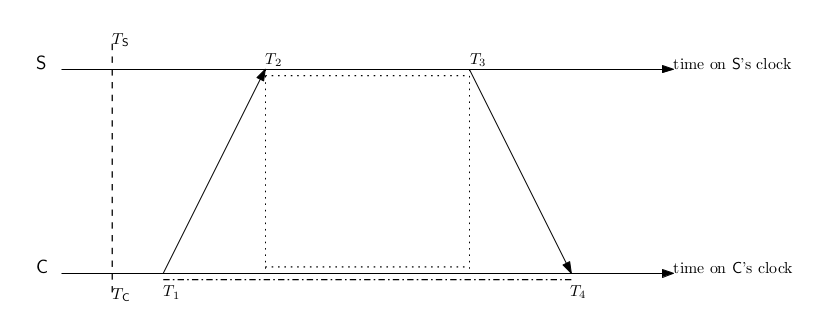
\includegraphics[width=.9\linewidth]{Synchronous Agreement (7)/screenshot_2018-09-23_08-58-10.png}
\end{center}
\begin{itemize}
\item When a client wants to synchronize its clock the following protocol is executed
\begin{enumerate}
\item \(C\) sends a time request message to \(S\) and stores its current system time \(T_1\)
\item Upon receiving the time request message, the server \(S\) stores its current system time \(T_2\)
\item The server \(S\) prepares a time response message which includes the time \(T_2\). Right before sending the response to the client \(C\), the server \(S\) measure its current system time \(T_3\) again and includes its in the message
\item Upon receiving the message \((\text{time response}, T_2,T_3)\), the client \(C\) messures its current system time \(T_4\). It can now compute two numbers:
\end{enumerate}
\end{itemize}
\begin{equation}
  \begin{split} 
    \text{TransEst} &= \frac{(T_4-T_1)-(T_3-T_2)}2 \\
   \text{OffsetEst} &= (T_1) + \text{TransEst} - T_2
  \end{split}
\end{equation}
\begin{itemize}
\item and adjusts its own clock using this number

\item The client often speeds up the clock a bit to set the clock correct since sudden jumps forward or backward in time can cause problems

\item To accommodate the problem of potential errors when transferring the protocol the client typically runs the protocol several times and takes the execution where \(\text{TransEst}\) was lowest
\begin{itemize}
\item To make sure that assumption 2 is probably true
\item The rational is that when transfer errors happens the transmission times tend to be higher
\end{itemize}
\end{itemize}

\subsection{Round-Based Protocols}
\label{sec:orgd36e92e}
\begin{itemize}
\item A \textbf{fully synchronous round-based model} in the simplest instantiation
\begin{itemize}
\item It has \(n\) parties or process called \(P_1,\dots,P_n\).
\item The protocol \(\pi\) proceeds in rounds
\item The idea is that in each round each process is allowed to send a message to each other process
\begin{itemize}
\item Send nothing is an option which is denoted NOMSG
\end{itemize}
\item In this model it is assumed that all processes have perfectly synchronized clock and transmission time is fixed
\item It is hardly realistic
\item Though even if clocks are not perfectly synchronized we can still hope to set bounds on clock drift and transmission time and predict when a message ought to arrive
\begin{itemize}
\item If a client expects that a server will send a message at time \(t\)
\item It knows that its offset from the servers clock is at most \(\text{Offset}\)
\item It knows that it takes at most \(\text{Trans}\) seconds to send a message
\item Then it can conclude that no message was send if nothing was received at time \(t + 2\text{Offset} + \text{Trans}\)
\end{itemize}
\end{itemize}

\item Generalizing this idea to a protocol \(\pi\) consisting of many rounds
\begin{itemize}
\item The bounds assumed is
\begin{itemize}
\item The computation that needed to be done in each takes the same time in each round, which is denoted \(\text{MaxComp}\)
\item The positive time bound \(\text{MaxTrans}\) on how long it maximally takes to send a message between two correct process
\item The positive time bound \(\text{MaxDrift}\) on how long any correct process drifts from real time is assumed
\end{itemize}
\item The \(\text{SlotLength}\) can be computed as \(\text{SlotLength}=2\text{MaxDrift} + \text{MaxTrans} + \text{MaxComp}\)
\begin{itemize}
\item The time \(t_0\) is the time which all parties start running the protocol
\item Each round runs within the a time slot
\item Rounds are index by natural numbers \(r\)
\item Let \(\text{SlotBegin}^r = t_0 + r \cdot \text{SlotLength}\)
\item Let \(\text{SlotEnd}^r=t_0+(r+1) \cdot \text{SlotLength}\)
\item Round \(r\) is assigned the time slot \(\text{Slot}^r = [ \text{SlotBegin}^r, \text{SlotEnd}^r )\)
\end{itemize}
\item A round based protocol proceeds as follows
\begin{enumerate}
\item Each \(P_i\) starts round \(r=0\) at time \(\text{SlotBegin}^0 = t_0\) 
\begin{itemize}
\item At time \(\text{SlotEnd}^0\) the computation of round \(0\) should have terminated
\item Let \((m_{i,1}^0, \dots m_{i,n}^0)\) be the messages to be send
\item For each \(P_j\), send \(( \text{MSG}, 0, m_{i,j}^0)\) to \(P_j\)
\end{itemize}
\item In rounds \(r=1,2,\dots\), party \(P_i\) runs as follows:
\begin{enumerate}
\item On message from \(( \text{MSG}, r-1, m)\) from \(P_j\) after timer \(\text{SlotBegin}^r-2 \text{MaxDrift}\) and before \(\text{SlotBegin}^r + \text{MaxTrans} + 2 \text{MaxDrift}\) if this the first message of the form \(( \text{MSG}, r-1, \cdot)\), then store \(m_{j,i}^{r-1} = m\)
\item At time \(\text{SlotBegin}^r + \text{MaxTrans} + 2\text{MaxDrift}\), for each \(P_j\) where no \(m_{j,i}^{r-1}\) is stored
\begin{itemize}
\item Define \(m_{j,i}^{r-1} = \text{NOMSG}\)
\item Using as input the values \((m_{1,i}^{r-1}, \dots m_{n,i}^{r-1})\) now stored and defined, perform whatever computation \(\pi\) prescribes for round \(r\)
\end{itemize}
\item At time \(\text{SlotBegin}^r + \text{MaxTrans} + 2 \text{MaxDrift} + \text{MaxComp}\)
\begin{itemize}
\item The computation of round \(r\) should have terminated
\item Let \((m_{i,1}^r, \dots m_{i,n}^r)\) be the messages to be send
\item For each \(P_j\), send \$(\text{MSG}, \(r\), m\(_{\text{i,j}}^{\text{r}}\))\$ to \(P_j\).
\end{itemize}
\end{enumerate}
\end{enumerate}
\item If in round \(r-1\) a correct \(P_j\) send \((\text{MSG},r-1,m)\) to \(P_i\) before \(\text{SlotBegin}^{r-1} + \text{MaxTrans}+ 2\text{MaxDrift} + \text{MaxComp}\) and the message was received too late by \(P_i\) such that \(m_{j,i}^{r-1}=\text{NoMsg}\) in round \(r\) it is said that the correct message was dropped by timeout
\begin{itemize}
\item If the assumptions on the timebounds are all correct this will never happen
\end{itemize}
\end{itemize}
\end{itemize}

\subsection{Unscheduled Consensus Broadcast using Signatures}
\label{sec:org70659f3}
\begin{itemize}
\item In \textbf{consensus broadcast}, some broadcaster sends a message to all other parties
\begin{itemize}
\item It must be guaranteed that all correct parties receive the same message, even if the broadcaster and some of the receivers are corrupted
\item Sometime called just \textbf{broadcast} or \textbf{consensus}
\end{itemize}

\item \textbf{Scheduled broadcast} is a type consensus broadcast
\begin{itemize}
\item The broadcast happens in a planned round
\item All parties known that it will happen at the specified round
\end{itemize}

\item \textbf{Unscheduled broadcast} is a another type consensus broadcast
\begin{itemize}
\item The broadcast can be initiated by the broadcaster in any round
\end{itemize}

\item \textbf{Unscheduled Consensus Broadcast} is a protocol between \(n\) parties \(P_1, \dots, P_m\)
\begin{itemize}
\item A party \(P_i\) can get inputs of the form \((\text{Send},m)\)
\begin{itemize}
\item If it is correct, it get this input at most one for each \(m\)
\end{itemize}
\item A party \(P_j\) can give outputs of the form \((\text{Deliver},P_i,m)\).
\item The following properties are important
\begin{itemize}
\item \textbf{Validity:} If a correct \(P_j\) outputs \((\text{Deliver},P_i,m)\), and \(P_i\) is correct, then at some point \(P_i\) got the input \((\text{Send},m)\)
\item \textbf{Agreement:} If a correct \(P_j\) outputs \((\text{Deliver},P_i,m)\), then eventually every correct \(P_j\) outputs \((\text{Deliver},P_i,m)\)
\item \textbf{Timing:}
\begin{itemize}
\item If a correct \(P_i\) gets input \((\text{Send},m)\) then all correct \(P_j\) output \((\text{Deliver}, P_i,m)\) in the next round.
\item If a correct \(P_j\) outputs \((\text{Deliver}, P_i, m)\) in round \(r_j\) and a correct \(P_k\) outputs \((Deliver, P_i, m)\) in round \(r_k\), then \(|r_k-r_j| \leq 1\).
\end{itemize}
\end{itemize}
\item The Validity and Agreement properties are safety properties
\item The Timing property is neither a safety property or a liveness property
\item Uses digital signatures
\begin{itemize}
\item Each party \(P_i\) has a publicly known verification key \(\text{vk}_i\) for a signature chee
\item Only \(P_i\) knows the signing key \(\text{sk}_i\)
\item It is important that all process agrees on the verification keys \(\text{vk}_i\) for all process
\begin{itemize}
\item It is assumed that the round based protocol have a initialization round where all parties broadcast the public keys.
\item In practice there are no such round
\end{itemize}
\end{itemize}
\end{itemize}

\item It is assumed that all round based protocol run the following code in round 0:
\begin{itemize}
\item \textbf{initialize} In round \(0\) each party \(P_i\) samples a key-pair \((\text{vk}_i,\text{sk}_i) \rightarrow \text{Gen}(1^k)\), and broadcasts \(\text{vk}_i\)
\begin{itemize}
\item \(k\) is the security parameter
\item These keys are delivered in one round
\item All parties in the futher use \(\text{vk}_i\) as the verification key of \(P_i\)
\end{itemize}
\end{itemize}

\item The unscheduled round based protocol is as follows
\begin{itemize}
\item \textbf{send} \(P_i\): On input \((\text{Send},m)\), compute \(\sigma_i=\text{Sig}_{\text{sk}_i}(Send,m)\) and send \((\text{Send},m,P_i,\sigma_i)\) to all parties
\item \textbf{deliver} \(P_j\): On input \((\text{Send},m,P_i,\sigma_i)\), if \((\text{Deliver}, P_i, m)\) was not output before, output \((\text{Deliver},P_i,m)\) and send \((\text{Send},m,P_i,\sigma_i)\) to all parties
\end{itemize}
\end{itemize}

\subsection{Consensus Broadcast using Authenticated Channels}
\label{sec:org88e9be6}
\begin{itemize}
\item In the \textbf{Authenticated Channels model} when \(P_i\) receives message \(m\) from \(P_j\), he knows that \(m\) really came from \(P_j\)
\begin{itemize}
\item If \(P_i\) is corrupt he may later choose to lie and claim that the got some other message from \(P_j\)
\item MACs are used between each pair of parties
\end{itemize}

\item A protocol for Scheduled Consensus Broadcast starts in a particular globally known round and takes place between \(n\) parties \(P_1, \dots, P_n\)
\begin{itemize}
\item There is a designated party known as the broadcaster
\item \(P_1\) is the broadcaster
\item The input of \(P_i\) is a message \(m \in \{0,1\}^*\)
\item The output of \(P_i \ne P_1\) is a result \(r_i \in \{0,1\}\)
\item For \(P_1\) we define \(r_1=m\)
\item At the beginning of the protocol \(r_i = \bot\) for all correct processes \(P_i \ne P_1\)
\item When \(P_i\) is ready to give an output it sets \(r_i\) to a value in \(\{0,1\}^*\) and never changes it again
\item A protocol is said to be executed correctly if all correct processes started running the protocol in the same round
\item The following properties are imposed on correctly executed protocols:
\begin{itemize}
\item \textbf{Validity:} If \(P_1\) is correct, then it holds for each correct process \(P_i \ne P_1\) that \(r_i=m\)
\item \textbf{Agreement:} It holds for each pair \(P_i\) and \(P_j\) of correct processes that are not \(P_1\) that is \(r_i \ne \bot\) and \(r_j \ne \bot\) then \(r_i = m\)
\item \textbf{Termination:} There exists some constant \(cc\) such that whenever the protocol starts executing in round \(t_0\), then by round \(t_0 + c\) it holds for all correct \(P_i\) that \(r_i \ne \bot\)
\end{itemize}
\item Termination and Agreement should hold even if \(P_1\) is not valid
\item All properties must hold even if some of the process are not valid
\end{itemize}

\item The protocol for \textbf{Scheduled Consensus Broadcast} which works four parties of which at most one cat be Byzantine
\begin{enumerate}
\item In round 1 party \(P_1\) sends \(m\) to \(P_2, P_3, P_4\)
\item Let \(m_i\) be the message received by \(P_\) in round 1. In round two party \(P_i\) sends \(m_i\) to \(P_2,P_3, P_4\).
\item Let \(m_{j,i}\) be the message received by \(P_i\) from \(P_j \ne P_1\) in round 2.
\begin{itemize}
\item By definition let \(m_i,i=m_i\)
\end{itemize}
\item In round 3 party \(P_i \ne P_1\) does the following:
\begin{itemize}
\item If there is a message \(h\) such that \(h\) occurs twice in \((m_{2,i},m_{3,i},m_{4,i})\) then let \(r_i = h\)
\item Otherwise, set \(r_i\) to a special error message and then halt.s
\end{itemize}
\end{enumerate}
\end{itemize}

\subsection{Byzantine Agreement using Authenticated Channels}
\label{sec:orge1fdfc2}
\begin{itemize}
\item The Byzantine Agreement is a protocol between \(n\) parties, which is denoted as \(P_1, \dots P_n\)
\begin{itemize}
\item The input of \(P_i\) is a vote \(v_i \in \{0,1\}\)
\item The output of \(P_i\) is a result \(r_i \in \{0,1\}\)
\begin{itemize}
\item At the beginning of the protocol we set \(r_i = \bot\) for all correct processes
\end{itemize}
\item When \(P_i\) is ready to give an output it sets \(r_i\) to \(0\) or \(1\) and then never changes it again
\item The protocol was executed correctly if all the correct process started running the protocol the same round
\item The following properties are imposed on correctly executed protocols
\begin{itemize}
\item \textbf{Validity:} It holds for each correct \(P_i\) that if \(r_i \ne \bot\) then there exists a correct process \(P_j\) such that \(r_j = v_j\)
\item \textbf{Agreement:} It holds for each pair \(P_i\) and \(P_j\) of correct processes that if \(r_i \ne \bot\) and \(r_j \ne \bot\) then \(r_i = r_j\)
\item \textbf{Termination:} There exists some constant \(c\) such that whenever the protocol starts executing in round \(t_0\), then by round \(t_0 + c\) it holds for all correct \(P_i\) that \(r_i \ne \bot\)
\end{itemize}
\item To work with Byzantine agreement one must always assume that \(t < n/2\)  byzantine corrupted
\end{itemize}
\end{itemize}

\subsection{Dolev-Strong: Scheduled Broadcast using Signatures}
\label{sec:orga28f420}
\begin{itemize}
\item A solution which works for any \(n\) and any \(t< n\)
\item \(P_1\) is the broadcaster
\item The protocol makes use of variables of form \(\text{Relayed}_i(m)\)
\begin{itemize}
\item This flag signals whether \(P_i\) has seen a signature from the broadcaster \$P\(_{\text{1}}\)\$on message  \(m\) and has relayed it to the other player
\end{itemize}

\item \textbf{initialize} In round \(0\) party \(P_i\) samples a key-pair \((vk_i,sk_i) \leftarrow \text{Gen}(1^k)\) where \(k\) is the security parameter
\begin{itemize}
\item All parties \(P_i\) set \(\text{Relayed}_i(m) = \bot\) for all possible message \(m\) from the message domain
\end{itemize}

\item \textbf{broadcast}
\begin{itemize}
\item On input \(m\) in round \(1\)
\begin{itemize}
\item Party \(P_1\) computes \(\sigma_1 \leftarrow \text{Sig}_{sk_1}(m)\) and sends \((m, \{\sigma_1\})\) to all parties.
\item Set \(r_1=m\), set \(\text{Relayed}_1(m) = \top\) and halt
\end{itemize}
\item In round \(r\), if \(Pi\) receives a message of form \((m, \Sigma)\) where \(\Sigma\) is a set of signatures and if \(\text{Relayed}_i(m)=\bot\) proceed as follows:
\begin{itemize}
\item Call \(\Sigma\) valid for \(m\) in round \(r\) if it contains signatures \(\sigma_j\) from \(r-1\) distinct parties \(P_j\) such that \(\text{Vec}_{vk_j}(m,\sigma_j) = accept\)
\item One of the parties have to be \(P_1\)
\item If \(\Sigma\) is valid for \(m\) in round \(r\), then compute \(\sigma_i \leftarrow \text{Sig}_{sk_i}(m)\), let \(\Sigma' \leftarrow \sigma \cup \{\sigma_i\}\)  and send \((m,\sigma')\) to all parties. Then set \(\text{Relayed}_i(m)= \top\)
\end{itemize}
\item In round \(n+2\) party \(P_i\) computes its output as follows:
\begin{itemize}
\item If there is exactly one message \(m\) such that \(\text{Relayed}_i(m) = \top\), then set \(r_i = m\)
\item Otherwise, set \(r_i = NoMsg\)
\end{itemize}
\end{itemize}
\end{itemize}

\subsection{Lower Bound on Round-Complexity of Broadcast using Signatures}
\label{sec:org2c99f01}
\begin{itemize}
\item To tolerate \(t<n\), then one can make a protocol which only runs in \(t+1\) rounds fulfilling these conditions
\begin{enumerate}
\item After some round of initialisation, the protocol only uses point to point communication
\item Ignoring the probability that the signature schemes could be broken the protocol is perfect
\begin{itemize}
\item i.e. validity,termination and agreement hold with probability 1
\end{itemize}
\end{enumerate}
\end{itemize}

\textbf{Theorem 7.1} Consider a deterministic protocol for \(n\) parties where all parties terminate in round \(r\). Assume that up to \(t\) parties might be crash-silent corrupted and that \(n \geq t+2\). If the system achieves weak Byzantine agreement, then \(r \geq t+1\)  

\section{Asynchronous Agreement (8)}
\label{sec:org6ac48d6}
\subsection{Byzantine Asynchronous Broadcast using Authenticated Channels}
\label{sec:org2b8a711}
\begin{itemize}
\item A Byzantine broadcast protocol for the full connected model with authenticated channels and asynchronous communication with eventual delivery
\item There are \(n\) parties \(P_1, \dots, P_n\)
\begin{itemize}
\item All can act as the bradcaster
\item \(P_1\) is assumed to always be the broadcaster
\item The broadcaster can get input of the form \((\text{BROADCAST}, P_1, bid, m)\), where \(bid\) is a fresh broadcast identifier
\item Other parties can give outputs of the form \((\text{DELIVER}, P_1, bid, m')\)
\end{itemize}

\item The requirements for the protocol:
\end{itemize}
\begin{center}
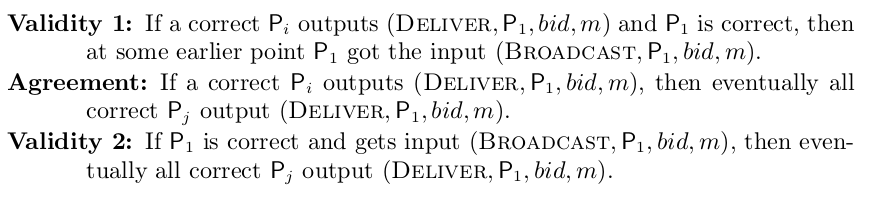
\includegraphics[width=.9\linewidth]{Asynchronous Agreement (8)/screenshot_2018-09-29_16-58-36.png}
\end{center}

\begin{itemize}
\item Let \(n\) be the number of parties and let \(t <n/3\) be the number of Byzantine corruptions to tolerate. A protocol for this is know as Bracha broadcast:
\end{itemize}
\begin{center}
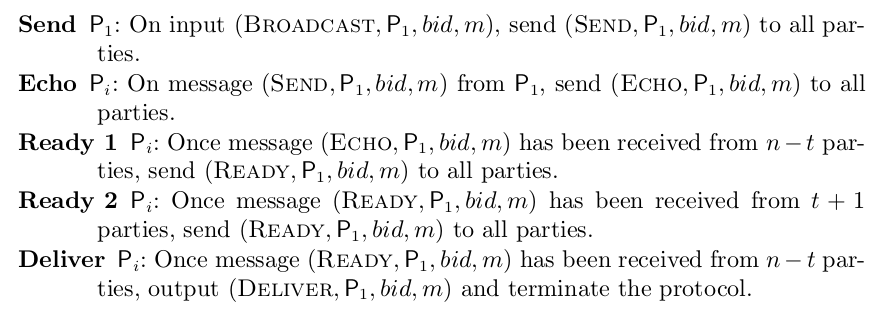
\includegraphics[width=.9\linewidth]{Asynchronous Agreement (8)/screenshot_2018-09-29_17-02-13.png}
\end{center}

\begin{itemize}
\item Waiting for a message from \(n-t\) process gives the process the most information possible without deadlocking
\item Waiting for a message from \(t+1\) parties ensures that one hears from at least one correct party
\item \(n<3t\) guarantee that there is at least one shared correct party that any two of the correct process heard from
\item If \(P_1\) is corrupt and does not send its message, then the correct parties run forever
\end{itemize}

\subsection{Impossibility of Deterministic Asynchronous Byzantine Agreement}
\label{sec:orgdafc73c}
\begin{itemize}
\item Each Byzantine agreement will be identified by a fresh identifier \emph{baid}
\begin{itemize}
\item Each party can get an input \((\text{VOTE}, baid, v_i)\) where \(v_i \in \{0,1\}\) is called the vote
\item Each party can give an output \((\text{DECISION}, baid,d_i)\) \(d_i \in \{0,1\}\) is called the decision
\end{itemize}

\item Requirements:
\end{itemize}
\begin{center}
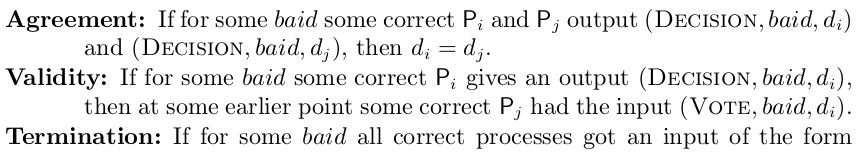
\includegraphics[width=.9\linewidth]{Asynchronous Agreement (8)/screenshot_2018-09-29_17-26-26.png}
\end{center}
\begin{center}
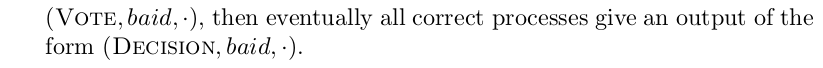
\includegraphics[width=.9\linewidth]{Asynchronous Agreement (8)/screenshot_2018-09-29_17-26-49.png}
\end{center}
\begin{itemize}
\item It is impossible to make a deterministic protocol which can handle one crash silent error for Byzantine agreement
\end{itemize}

\subsection{Possibility of Randomised Asynchronous Byzantine Agreement}
\label{sec:org46c1ae6}
\subsubsection{Weak Agreement}
\label{sec:orgb2d91a5}
\begin{itemize}
\item Byzantine agreement in the asynchronous model
\begin{itemize}
\item Each Byzantine agreement ill identified by a fresh identifier \emph{baid}
\item Each party can get an input \((\text{VOTE}, baid, v_i)\) where \(v_i \in \{0,1\}\) is called a vote
\item Each party can give an output \(\text{DECISION}, baid, d_i\) where \(d_i \in \{0,1,?\}\)
\begin{itemize}
\item The output \(?\) signals that an agreement could not be reached
\item If some party output \(0\) then all other parties output \(0\) or \(?\) and the same for \(1\)
\item If all parties vote the same no party is allowed to output \(?\)
\end{itemize}
\end{itemize}

\item Requirements:
\end{itemize}
\begin{center}
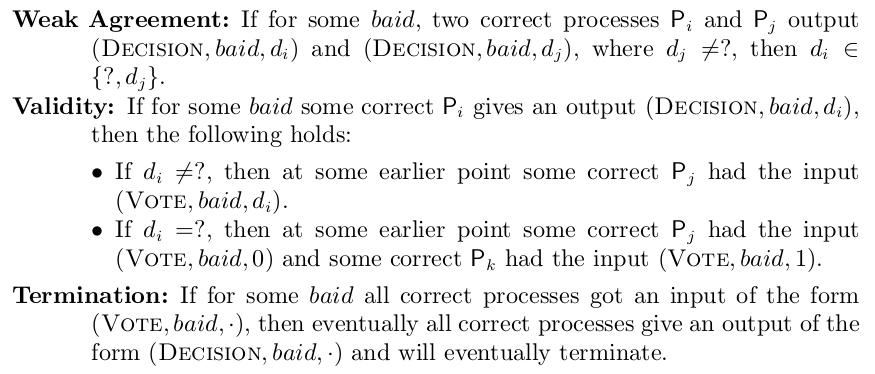
\includegraphics[width=.9\linewidth]{Asynchronous Agreement (8)/screenshot_2018-09-29_17-47-32.png}
\end{center}

\begin{itemize}
\item A protocol that works for \(n> 5t\) using only authenticated channels
\end{itemize}
\begin{center}
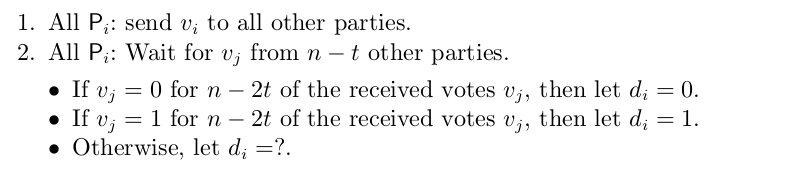
\includegraphics[width=.9\linewidth]{Asynchronous Agreement (8)/screenshot_2018-09-29_17-49-39.png}
\end{center}

\begin{itemize}
\item The protocol has \textbf{termination} since there are at most \(t\) corrupted parties, so the \(n-t > n-2t\) message in step 2 will eventually arive
\item It has \textbf{validity} since if all correct parties has the same input \(v\) then all parties will receive at least \(n-2t\) votes for \(d\) and therefore \(d_i = d\)
\end{itemize}

\subsubsection{From Weak Agreement to Agreement}
\label{sec:org3f82a27}
\begin{itemize}
\item To get Byzantine agreement from Weak Byzantine Agreement the following protocol is considered
\end{itemize}
\begin{center}
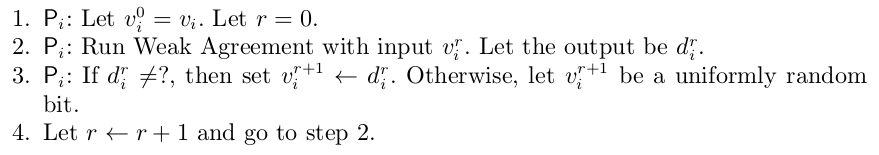
\includegraphics[width=.9\linewidth]{Asynchronous Agreement (8)/screenshot_2018-09-29_17-58-43.png}
\end{center}

\begin{itemize}
\item A network has \textbf{stabilised} on \(v \in \{0,1\}\) ins round \(r\) if it holds for all correct \(P_i\) that \(v_i^r=v\)
\begin{itemize}
\item There is a non-zero probability in each round that the network will stabilise
\end{itemize}
\end{itemize}

\subsubsection{Graded Agreement}
\label{sec:orgbb992bf}
\begin{itemize}
\item Graded agreements is an extension of weak agreement
\item There are two possible outputs for \(0\), \((0,1)\)  and \((0,2\) )
\begin{itemize}
\item The second component is the grade
\item If someone outputs \((0,2)\) then all other parties output \((0,2)\) or \((0,1)\), similar with \((1,2)\)
\item A decision with grade \(2\) allows to conclude that all parties made the same decision
\item If the output is \(?\) the grade is always \(0\)
\item Possible outputs: \((0,2),(0,1), (?,+), (1,1), (1,2)\)
\end{itemize}

\item The syntax is as follows
\begin{itemize}
\item Parties can have inputs of the form \((\text{VOTE}, baid, v_i)\) where \emph{baid} is a fresh BA identifier and \(v_i \in \{0,1\}\) is a vote
\item Parties can have outputs of the form \((\text{DECISION}, baid, d_i, g_i)\), where \(d_i \in \{0,?,1\}\) is a decision and \(g_i \in \{0,1,2\}\) is a grade
\item Each possible output is assigned to a number according to the ordered list \(n(0,2) = 1, n(0,1) = 1, \dots, n(1,2) =5\)
\end{itemize}

\item The requirements
\end{itemize}
\begin{center}
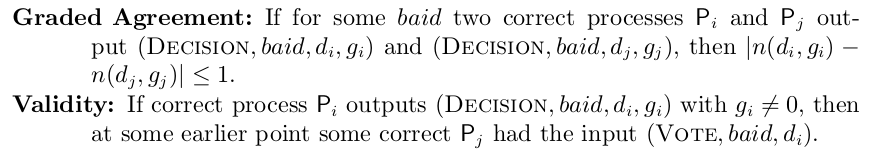
\includegraphics[width=.9\linewidth]{Asynchronous Agreement (8)/screenshot_2018-09-29_18-14-58.png}
\end{center}
\begin{center}
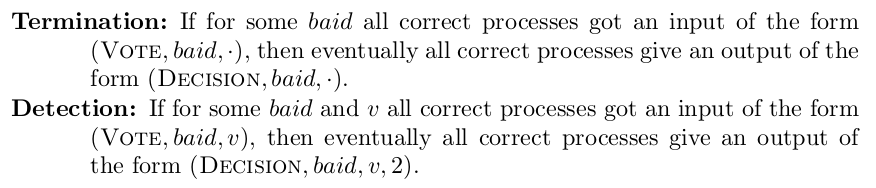
\includegraphics[width=.9\linewidth]{Asynchronous Agreement (8)/screenshot_2018-09-29_18-15-21.png}
\end{center}

\begin{itemize}
\item A protocol which works for \(n > 9t\)
\end{itemize}
\begin{center}
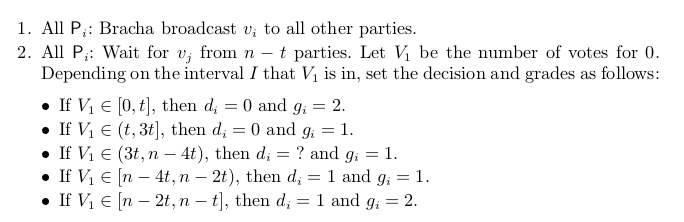
\includegraphics[width=.9\linewidth]{Asynchronous Agreement (8)/screenshot_2018-10-04_10-40-32.png}
\end{center}
\begin{itemize}
\item The ones with a question \(?\) chooses a new vote \(0,1\) at random
\end{itemize}
\begin{center}
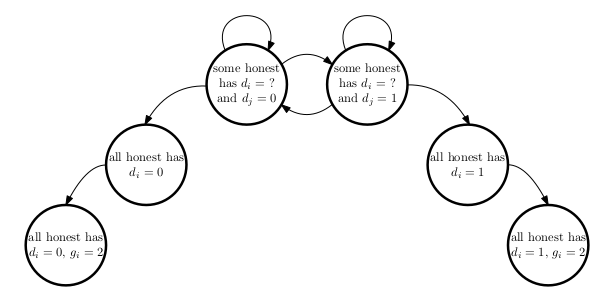
\includegraphics[width=.9\linewidth]{Asynchronous Agreement (8)/screenshot_2018-10-04_10-57-29.png}
\end{center}

\subsubsection{From Graded Agreement to Terminating Agreement}
\label{sec:org63f802e}
\begin{itemize}
\item The termination that one want is typically that all resources allocated to a terminate process is not free
\begin{itemize}
\item Such as in Bracha Broadcast
\end{itemize}

\item It could be dangerous terminating all sub-protocols, since some correct processes \(P_j\) might be arbitrarily behind
\begin{itemize}
\item If a process \(P_i\) terminates before \(P_j\) "wakes up", then \(P_i\) will not be around to participate in the sub protocol
\end{itemize}

\item The main trick used is that when honest parties terminate and shut down, they send messages that will later inform slow correct processes about the result of the computation when they wake up
\begin{itemize}
\item They are called \textbf{time capsule messages}
\item They are sent before \(P_i\) terminates
\item They will be around to be picked up by \(P_j\) when it wakes up
\end{itemize}

\item \textbf{Definition 8.1 (Asynchronous Termination).} When we say that a party terminates, we mean that it terminates its own process, plus its processes in any subprotocol it started. There is one important exception: it will forever keep running the process that implements the authenticated channels it is using.
\begin{itemize}
\item Could be done by having the operating system of the computer handle the sending and receiving of messages
\item When a correct process terminates it cannot affect the liveness of the protocol it participated in namely the safety property
\end{itemize}

\item The following protocol assumes a protocol for Graded Byzantine Agreement and implements Byzantine Agreement with Asynchronous Terminatation
\begin{itemize}
\item It works if \(n>3t\) and if the Graded BA is secure for the same \(t\) and \(n\)
\end{itemize}
\end{itemize}
\begin{center}
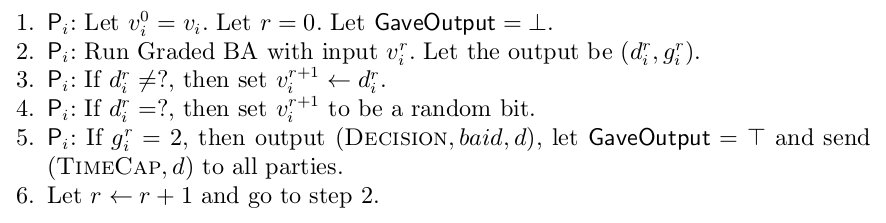
\includegraphics[width=.9\linewidth]{Asynchronous Agreement (8)/screenshot_2018-09-30_08-25-11.png}
\end{center}

\begin{itemize}
\item I addition to the other rules the parties also run the following extra rules:
\end{itemize}
\begin{center}
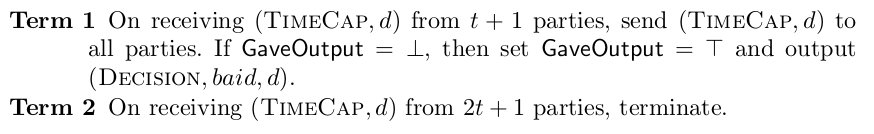
\includegraphics[width=.9\linewidth]{Asynchronous Agreement (8)/screenshot_2018-09-30_08-26-08.png}
\end{center}

\subsection{Weak Multi-Valued Byzantine Agreement}
\label{sec:org72817cb}
\begin{itemize}
\item \textbf{Weak Multi-Valued Byzantine Agreement} allows one to use Byzantine Agreement for much larger decisions than 1 bit 
\begin{itemize}
\item It is called weak since it is not guaranteed to agree on an input of an honest party
\item If it decides on a value that was not a correct input, then it is a special error symbol \(\bot\)
\end{itemize}

\item Each Byzantine pre-agreement will be identified by a fresh identifier \emph{baid}
\begin{itemize}
\item Each party can get an input \((\text{VOTE}, baid, v_i)\), where \(v_i \in \{0,1\}^*\) is called the proposal
\item Each party can give an output \((\text{DECISION}, baid, d_i)\), where \(d_i \in \{0,1\}^* \cup \{\top\}\) is called the decision
\item The properties required are
\end{itemize}
\end{itemize}
\begin{center}
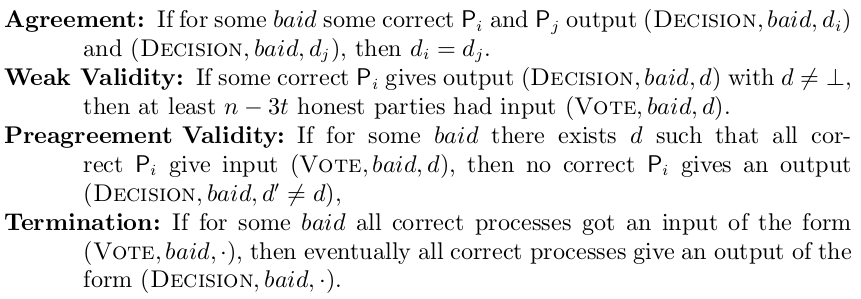
\includegraphics[width=.9\linewidth]{Asynchronous Agreement (8)/screenshot_2018-09-30_08-47-49.png}
\end{center}

\begin{itemize}
\item In the protocol there are \(n\) parties and a parameter \(t < n/5\)
\begin{itemize}
\item There are at most \(t\) maliciously faulty parties
\item The protocol uses a BA protocol which is assumed secure for the parameters
\item The protocol:
\end{itemize}
\end{itemize}
\begin{center}
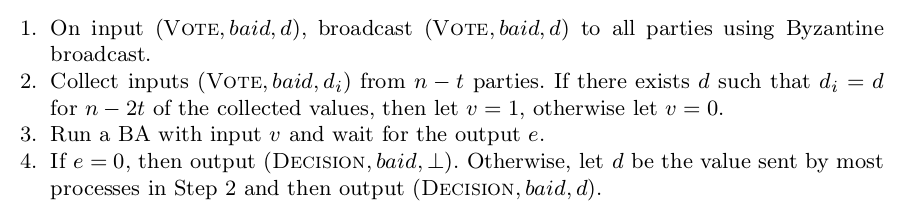
\includegraphics[width=.9\linewidth]{Asynchronous Agreement (8)/screenshot_2018-09-30_08-52-14.png}
\end{center}

\section{Key Management and Infrastructures (9)}
\label{sec:orga3ede1f}
\subsection{General}
\label{sec:org7cd52ad}
\begin{itemize}
\item When solving the problem of distributing keys one has to be aware of the following problem: \emph{Any secret system parameter runs a greater risk of being revealed, the longer time you keep it constant, and the more you use it}
\begin{itemize}
\item It is good practise to change the keys one uses at regular intervals
\end{itemize}
\end{itemize}

\subsection{Two-party Communication}
\label{sec:orgd4ad12d}
\begin{itemize}
\item The standard way for achieving confidentiality (or authenticity or both) in two-party communication between \(A\) and \(B\) is to have a key \(K_{AB}\) agreed between \(A\) and \(B\) initially which is used for sending keys from \(A\) to \(B\)
\begin{itemize}
\item To send a message \(M\), \(A\) will generate a random \texttt{session} key \(k\) and send \(E_{K_{AB}}(K), E_k(M)\) to be
\begin{itemize}
\item \(K\) will be used for multiple messages but deleted after a short time e.g. when the connection is closed
\end{itemize}
\item The argument for using this system is to avoid given a potential adversary a very large amount of data encrypted under one key which makes the crypt-analysis easier
\item To solve the problem for multiple users one would need another solution since the number of keys needed to manage would grow quadratically with the number of users
\end{itemize}
\end{itemize}

\subsection{Key Distribution Centers (KDC)}
\label{sec:org4227a6f}
\begin{itemize}
\item \textbf{Key Distribution Centers} (KDC) are based only on secret-key technology
\begin{itemize}
\item There are one KDC and many users
\item Every user \(A\) shares a key \(K_A\) with the KDC
\item When \(A\) wants to talk to \(B\), the KDC generates a key \(K\) for the session and send \(E_{K_A}(K)\) to \(A\) and \(E_{K_B}(K)\) to \(B\)
\begin{itemize}
\item Both parties can then recover \(K\) and communicate using this key
\end{itemize}
\item KDC solutions are not so common because of the single point of failure which the KDC represents because
\begin{itemize}
\item All users must trust the KDC completely, since the KDC can decrypt or forge all traffic if it decides to misuse its knowledge.
\item If the KDC is down, the entire secure communication systems becomes unavailable.
\end{itemize}
\end{itemize}
\end{itemize}

\subsection{Certification Authorities (CA)}
\label{sec:orgebf1f89}
\begin{itemize}
\item In the two player above the shared key \(K_{AB}\) could be replaced by a public key pair \((sk_B,pk_B)\) generated by \(B\)
\begin{itemize}
\item Only \(B\) knows \(sk_B\) and \(pk_B\) is public
\item \(A\) can send \(E_{pk_B}(K)\) to \(B\) where \(K\) is the session key
\begin{itemize}
\item This means no secret key needs to be shared initially but one still needs to ensure that \(A\) uses the correct public key
\end{itemize}
\end{itemize}

\item Assume one have an entity called a Certification Authority with its own key pair \((sk_{CA}, pk_{CA})\)
\begin{itemize}
\item Assume that we can ensure that all users get an authentic copy of \(pk_{CA}\)
\item One can then do the following:
\begin{itemize}
\item Each users \(A\) in the system must contact the CA in some way and send his public key \(pk_A\) to the CA
\item The way \(A\) identifies himself cannot be via cryptography only:
\begin{itemize}
\item Before \(A\) has registered \(A\) and the CA do not share any secret keys
\item The CA does not know any public key it can safely assume belongs to \(A\)
\end{itemize}
\item There are many ways for \(A\) to identify himself
\begin{itemize}
\item In rare cases \(A\) must show up in person
\item In other cases a pin code is sent to ½A\$ in paper mail and used to log into the website of the CA
\end{itemize}
\item If CA accepts the identity of the user it will issue a certificate which consists of
\begin{itemize}
\item A string \(ID_A\)
\item The public key \(pk_A\)
\item The CA's signature \(S_{sk_{CA}}(ID_A,pk_A)\) on the former two pieces of data
\end{itemize}
\item Once certificates are issued it is possible to set up a secure communication with necessarily involving the CA
\end{itemize}
\item If a user suspects that his private key has been compromised, it should be possible for him to report this and have his certificate revoked
\begin{itemize}
\item This means there must be an option to check whether a given certificate is still valid
\item The CA should implemented an on-line service for this purpose
\item The certificate should also contain a validy period as part of what is signed by the CA
\end{itemize}
\item A certificate is typically a long data record with for instance the following fields:
\begin{itemize}
\item Name of the certificate owner
\item Name of the CA who signed the certificate
\item Method used by CA to check identity of certificate owner
\item Date issued
\item Validity period
\item Rights and privileges of certificate owner.
\item Crypto algorithm to be used for checking this certificate
\item Crypto algorithm used by certificate owner
\item Public key of certificate owner
\item Signature of CA.
\end{itemize}
\item One can use different certificate authorities each others certificate public keys e.g. \(Cert_ {CA_1}(CA_2, pk_{CA_2})\)
\begin{itemize}
\item A more general way is to use certificate chains, which is an ordered list of certificates 
\begin{itemize}
\item Where the first entry is a certificate where \(CA_1\) certifies the public key of user in question, in the second entry \(CA_2\) certifies the public key of \(CA_1\) etc. until the last entry where \(CA_n\) certifies the public key of \(CA_{n-1}\)
\end{itemize}
\item Limitations of certificate chain
\begin{enumerate}
\item \(A\) should only trust the end point to the extent that he trust that every CA involved in the chain has not issued fake certificates
\item Do not remove the need for at least one public key to be known to users initially 
\begin{itemize}
\item In a practical situation, the way that it is ensure is that the required public keys are delivered to the user together with the software needed to generate keys an do encryption and signatures
\end{itemize}
\end{enumerate}
\end{itemize}
\end{itemize}
\end{itemize}

\subsection{Limitations on Key Management}
\label{sec:orge9f5269}
\begin{itemize}
\item \emph{Any secure system using cryptography must make use of one or more keys that are protected only by physical, non-cryptographic means}
\end{itemize}

\subsection{Password Security}
\label{sec:org82f38fe}
\subsubsection{General}
\label{sec:org0343340}
\begin{itemize}
\item Passwords are often the weakest link in the security chain because they have to be remembered by humans

\item There are (at least) 4 important security aspects of password security and therefore 4 types of attacks that one must protect against
\begin{itemize}
\item How is the password chosen?
\begin{itemize}
\item Can the adversary guess the password and verify his guess?
\end{itemize}
\item How is the password transmitted between the password user and verifier?
\begin{itemize}
\item Can the adversary get hold of the password while it is in transit?
\end{itemize}
\item How is the password stored by the password user?
\begin{itemize}
\item Can the adversary steal the password from the user?
\end{itemize}
\item How is the password stored by the password verifier?
\begin{itemize}
\item Can the adversary steal the password from the verifier?
\end{itemize}
\end{itemize}
\end{itemize}

\subsubsection{Choosing and guessing Passwords}
\label{sec:orgae1020d}
\begin{itemize}
\item In general if the password is chosen from a character set of size \(C\) and has length \(\ell\) then there are \(C^\ell\) possible passwords
\begin{itemize}
\item This number grows must faster as a function of \(\ell\) than as a function of \(C\)
\item There are practical limitations to the length and studies show that 12 digits seem to be the maximum one can expect anyone to enter correctly
\item The length of the password is not a quality by itself, since passwords that real people can remember are usually not uniformly distributed
\item Some systems test chosen passwords against a know list of "bad" passwords and refuses people to use them
\item One should limited the number of failed login attempts and lock the account to make it harder for the adversary to guess passwords
\begin{itemize}
\item This could create the a problem where the adversary makes the availability break down
\item A better idea is to have the system wait for some time after some failed login attempts before he is allowed to try again and make this time longer, the more failed attempts are maid
\end{itemize}
\end{itemize}
\end{itemize}

\subsubsection{Using and eavesdropping passwords}
\label{sec:orgbd30e5d}
\begin{itemize}
\item Stealing the password when it is used can take many forms
\begin{itemize}
\item Such as looking over someones shoulder
\item Passwords sent over a LAN are very easy to detect and grab
\begin{itemize}
\item e.g. hackers sitting at the local cafe intercepting other customers using the free wifi
\end{itemize}
\item Looking over someone's shoulder can also be done electronically using so called spyware where the code run on the victim's machine in some unnoticed way
\begin{itemize}
\item The problem will record passwords and send them to the attacker
\end{itemize}
\item Encrypting network traffic definitely helps
\end{itemize}
\end{itemize}

\subsubsection{Storing and stealing passwords, the user side}
\label{sec:orgcfc6cb5}
\begin{itemize}
\item Stealing the password can be easy if it is written down 
\begin{itemize}
\item There are other methods such as fool users into revealing their passwords under false pretenses
\begin{itemize}
\item Known as \textbf{social engineering}
\item One of the most effective attacks on real systems and preventing it is very difficult
\end{itemize}
\item A variant of social engineering is a \textbf{phishing attack} where one sends a mail to the victim claiming that you are his bank or instance
\begin{itemize}
\item The mails ask the user to following a link leading to a fake web page that claims to be his bank's
\item The user is then asked to type his user name and password, to "validate the account"
\end{itemize}
\end{itemize}
\end{itemize}

\subsubsection{Storing and stealing passwords, the verifier side}
\label{sec:org89e5f1c}
\begin{itemize}
\item Stealing passwords from the verifying party may also be possible
\begin{itemize}
\item In some bad cases systems store passwords in cleartext
\item Some systems such as UNIX store a user record containing username \(u\) and \(f(pw_u)\) where
\begin{itemize}
\item \(pw_u\) is the password of user \(u\)
\item \(f\) is a one-way function where it is easy to compute \(f(pw_u)\) from \(pw_u\) but it is hard to go in the opposite direction
\begin{itemize}
\item e.g. a hash function
\end{itemize}
\end{itemize}
\item If the attacker has the password file and a password \(pw\) that he thinks is the users passwords it is easy to verify by computing \(f(pw)\) and check if it occurs in the file
\item \emph{Password crackers} are programs that can crack some password files
\begin{itemize}
\item They use dictionaries with probable password and try to match them with entries in a given password file
\end{itemize}
\item There are three main countermeasures against the password cracker kind of attacks:
\begin{enumerate}
\item \emph{Educate the users to choose hard to guess passwords}
\item \emph{Slow the attacker down:} It is possible to make the life of the adversary harder by making sure that the function \(f\)
\begin{itemize}
\item is slow enough to slow down the number of attempts a password cracker can run per second
\item while being fast enough for the system to be efficient enough
\end{itemize}
\item \emph{Removing the single point of failure:} an increasingly common architecture for stored password is for the password to be hashed together with a secret key \(K\) which is stored on a different machine than the one storing the password hash
\begin{itemize}
\item The adversary must get hold of both the hashed password and the key \(K\) to be able to verify their guesses
\item Require the second server to be involved in every password verification attempt
\item When the user \(u\) register its password \(pw\) this is sent to the hashing server that computes \(y=f(K,pw)\) and returns this value to the authentication server that stores the pair \((u,y)\)
\begin{itemize}
\item When the user contacts the authentication server, it sends the received password \(pw'\) and the hashed password \(y\) to the hashing server who checks whether \(f(K,pw')=y\) or not
\end{itemize}
\end{itemize}
\end{enumerate}
\end{itemize}
\end{itemize}

\subsection{Hardware Security}
\label{sec:org8149c89}
\subsubsection{Why use secure hardware?}
\label{sec:orge24920c}
\begin{itemize}
\item Hardware units with some degree of physical security are useful in many secure systems
\begin{itemize}
\item The purpose is to prevent an adversary from getting hold of the secret keys
\item It is possible for an adversary to get a hold of a private signature key on a hard disk
\begin{itemize}
\item The adversary then has lots of time offline to try and find a password by trying all possibilities and testing them against the encrypted key
\item Is also a problem with magnetic stripe cards
\end{itemize}
\item If the key is inside a hardware unit a potential attacker cannot easily break into the hardware unit
\begin{itemize}
\item An adversary has to steal the hardware unit and needs time and money to break into the device
\end{itemize}
\end{itemize}
\end{itemize}

\subsubsection{Tamper-evident hardware and two-factor authentication}
\label{sec:org24c8174}
\begin{itemize}
\item It is interesting to have hardware units that are difficult to break into even if it is not impossible to do so
\begin{itemize}
\item It may still be useful in improving security as long as there is a significant cost, and if the attack will take some time and or may leave some trace on the device showing it was attacked
\item This type of hardware is often called \textbf{tamper-evident} hardware
\item Chip-cards are examples of such units
\begin{itemize}
\item They often come with their own computer on board
\begin{itemize}
\item The storage is physically protected such that access to using the keys on board should be only trough the cards own CPU
\end{itemize}
\item You must use the PIN code that opens the card and follow the communication protocol
\item They are not impossible to break into but it requires a skilled and determined attacker, it takes non-negligible time, and requires specialized equipment
\end{itemize}
\item The way these devices is programmed should be done carefully since it might reveal some information about the key
\end{itemize}

\item A primary application for tamper-evident hardware is for two-factor authentication
\begin{itemize}
\item The idea is that one authenticate a user in two ways: first by a password and second by checking that he has a certain hardware unit in his possession
\item Typically done by putting a secret key \(K\) inside the unit
\begin{itemize}
\item This key is also held by the verifying party
\item The verifier issues a challenge \(c\) (a nonce) which the user forward to the hardware unit, it the returns a response \(R(K,c)\) that is a function of both \(K\) and \(c\)
\item Typically it encrypts \(c\) under \(K\)
\item The response can clearly be verified by the other party and replay attacks will not work because the challenge will not be the same the next time
\item The response \(R(K,c)\) is often called a \textbf{one-time password}
\item In some cases the challenge \(c\) is replaced by the current time which frees the user from manually forwarding \(c\) to the device
\end{itemize}
\item It can still be attacked using \textbf{real-time phishing} where the adversary fools the user to go to his web page rather than that of the bank and log in there instead
\begin{itemize}
\item The adversary then logs into the bank at the same time
\end{itemize}
\end{itemize}
\end{itemize}

\subsubsection{Tamper-Resistant hardware}
\label{sec:org7e6e7c4}
\begin{itemize}
\item These are called \textbf{tamper resistant} or \textbf{tamper-proof} are much more difficult to break into than tamper evident hardware
\begin{itemize}
\item It is estimated that not even a well funded organization with expert knowledge can break into the device
\item Some of them have their own CPU, storage and battery back-up and can do all the standard cryptographic algorithms internally.
\item Banks use these units to protect particularly sensitive and long-lived data, such as PIN codes for credit cards.
\item Also CA’s use this kind of technology to store their private keys used for issuing
\end{itemize}
\end{itemize}

\subsection{Biometrics}
\label{sec:orgf9e9fbe}
\begin{itemize}
\item \textbf{Biometrics} is using the various physical characteristics of the person trying to get access
\begin{itemize}
\item It can take a number of different forms: it can scan your fingerprint, your eye, your face, or listen to your voice
\item The the major problem in this area is always to do the conversion to digital and the comparison such that 
\begin{itemize}
\item The system is tolerant enough to accept the good guys
\item The system is restrictive enough to reject the cheaters.
\end{itemize}
\item Biometrics can provide better access control for your private signature key
\begin{itemize}
\item It cannot replace cryptographic authentication
\end{itemize}
\item Once has to take into account the weakest link such as a database containing the measurement
\end{itemize}
\end{itemize}

\subsection{Preventing bypass of the system}
\label{sec:orgcf8e36b}
\begin{itemize}
\item It is important that the system cannot be bypassword
\begin{itemize}
\item I.e. it must not be possible to get to the resource without asking the system
\item If one has secure hardware available and the resource is a key this is not difficult
\begin{itemize}
\item Just put the key inside the hardware and make sure it cannot be output from the device
\end{itemize}
\item If no secure hardware is available, life is much more difficult
\begin{itemize}
\item This is the situation if one is designing security on a standard PC
\item If one want to protect a private key one can encrypt the key using the password as a key
\begin{itemize}
\item To ensure that what we encrypt with is of fixed length the password is often hashed using some standard hash function \(h\) and using 128 bits of the output as key
\item For a password \(pw\) and secret key \(sk\) what is stored is \(E_{h(pw)}(sk)\)
\end{itemize}
\item Since the number of possible password is often must possible that the \(2^{128}\) AES keysome precautions must be taken, so a potential attacker can't just try all possible possword
\begin{itemize}
\item A solution is to make the function \(h\) slow i.e. rather than having \(h\) to be a standard hash function we make many iterations of it
\item This means that the right users will be slowed down, but not to much, but the attacker will have a much hard time
\end{itemize}
\end{itemize}
\end{itemize}
\end{itemize}

\section{State Machine Replication (10)}
\label{sec:org73497af}
\subsection{General}
\label{sec:orga166275}
\begin{itemize}
\item Replication is to run a service on several computers and keep them consistent
\begin{itemize}
\item To give input to the system you give the input to at least one correct serve, which then will send it to the other servers
\item They all end up with an up-to-date copy of the service
\item There must be some mechanism in place which ensure that updates are applied in the same order at all replicates
\item If there is disagreements one needs to adopt the one that was sent by the most severs
\end{itemize}
\end{itemize}

\subsection{State Machines}
\label{sec:org6949756}
\begin{itemize}
\item The service is abstracted to be replicated by a state machine \(M\)

\item \textbf{Definition 10.1 (State Machine)} A state machine \(M\) which consists of: 
\begin{itemize}
\item A set \(\text{States}\)
\item A start state \(\text{State}_0 \in \text{States}\)
\item A set \(\text{Inputs}\)
\item A set \(\text{Outputs}\)
\item A transition function \(T: \text{States} \times \text{Inputs} \to \text{States} \times \text{Outputs}\)
\end{itemize}
\item A state machines starts in \(\text{State}_0\)
\begin{itemize}
\item When it was in state \(\text{State}_i\) and receives input \(x\) then it computes \((State_{i+1},y)=T(\text{State}_i,x)\), changes state to \(\text{State}_{i+1}\) and outputs \(y\)
\end{itemize}
\end{itemize}

\subsection{Replicated State Machines}
\label{sec:orgf357e0b}
\begin{itemize}
\item A replicated state machine is a protocol for \(n\) servers which makes them behave as if they are running one single state machine \(M\)

\item \textbf{Definition 10.2 (Replicated State Machine)} Let \(M\) be a state machine. A replicated state machine running \(M\) is specified via an ideal functionality \(\text{RSM}_M\) for \(n\) servers \(\mathsf{S}_1, \dots, \mathsf{S}_n\).
\begin{itemize}
\item The syntax is as follows:
\begin{itemize}
\item There is a protocol port \(\text{IO}_i\) for receiving inputs from server \(\mathsf{S}_i\) and giving outputs to \(\mathsf{S}_i\)
\item There is a special port \(\text{RECEIVED}_i\) for reporting what messages have been input to the ideal functionality by \(\text{S}_i\)
\item There is a special port \(\text{PROCESS}\) for specifying which messages to process next
\item There is a special port \(\text{DELIVER}_i\) for instructing the ideal functionality to deliver the next message to \(\mathsf{S}_i\)
\end{itemize}
\item The ideal functionality runs as follows:
\begin{itemize}
\item Upon initialization
\begin{itemize}
\item Let \(\text{State}=\text{State}_0\)
\item For each \(\text{IO}_i\), let \(Q_i\) be the empty queue
\begin{itemize}
\item \(Q_i\) is for the outputs for server \(\mathsf S_i\) which have not been delivered yet
\end{itemize}
\item Initialize \(\text{UnProcessed}\) to be the empty set
\end{itemize}
\item On input \(x\) on \(\text{IO}_i\), output \(x\) on \(\text{RECEIVED}_i\) and add \(x\) to \(\text{Unprocessed}\)
\item On input \(x\) on \$\text{PROCESS}\$m where \(x \in \text{UnProcessed}\)
\begin{enumerate}
\item Let \((\text{State}', y)=T(\text{State},x)\) and update \(\text{State}= \text{State}'\)
\item Add \(t\) into all the queues \(q_i\)
\item Remove \(x\) from \(\text{UnProcessed}\)
\end{enumerate}
\item On an input on \(\text{DELIVER}_i\) where \(Q_i\) is not empty, remove the front element \(y\) from \(Q_i\) and output \(y\) on \(\text{IO}_i\)
\end{itemize}
\end{itemize}

\item One can formulate a liveness property which says that if \(x\) is added to \(\text{UnProcessed}\), then it will eventually be processed and all outputs will eventually be delivered

\item An important safety property is that the outputs that the parties see is always the result of running from the initial state on some sequence of inputs that is the same for all parties. 
\begin{itemize}
\item Notice that the parties using \(RSM_M\) might not have seen the same number of these outputs.
\end{itemize}
\end{itemize}

\subsection{Totally-Ordered Broadcast}
\label{sec:org5f5d320}
\begin{itemize}
\item The main building block to implement state-machine replication is totally-ordered broadcast

\item \textbf{Definition 10.3 (Totally-Ordered Broadcast)} We specify the behavior of totally-ordered via an ideal functionality TOB for \(n\) parties \(\mathsf P_1, \dots, \mathsf P_n\)
\begin{itemize}
\item The syntax is as follows
\end{itemize}
\end{itemize}
\begin{center}
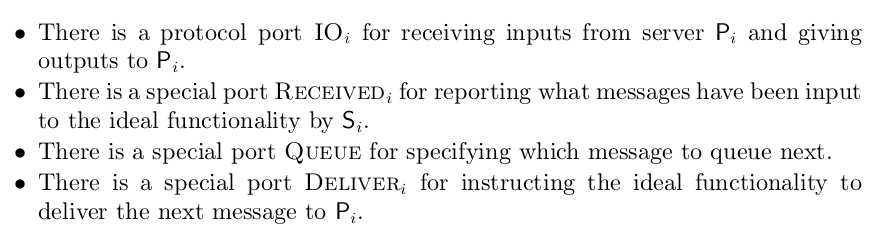
\includegraphics[width=.9\linewidth]{State Machine Replication (10)/screenshot_2018-10-21_08-51-18.png}
\end{center}
\begin{itemize}
\item The ideal functionality runs as follows
\end{itemize}
\begin{center}
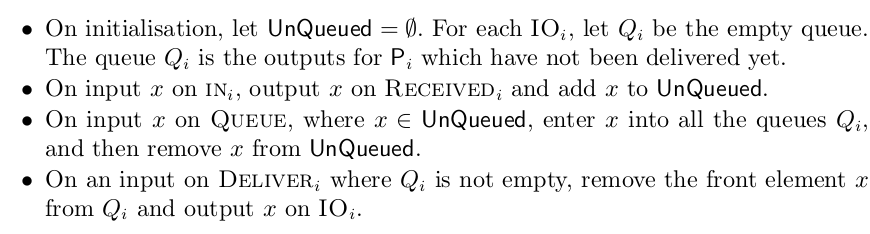
\includegraphics[width=.9\linewidth]{State Machine Replication (10)/screenshot_2018-10-21_08-51-36.png}
\end{center}

\begin{itemize}
\item To implement \(\text{RSM}_M\) given TOB one simply broadcast all inputs to all servers which then run the machine \(M\) on the agreed sequence
\begin{itemize}
\item Everyone runs the same machine on the same sequence of inputs and therefore all servers will end up in the same state
\end{itemize}

\item Replicated State Machine for \(M = (\text{States}, \text{State}_0 , \text{Inputs}, \text{Outputs})\) from Totally-Ordered Broadcast
\end{itemize}
\begin{center}
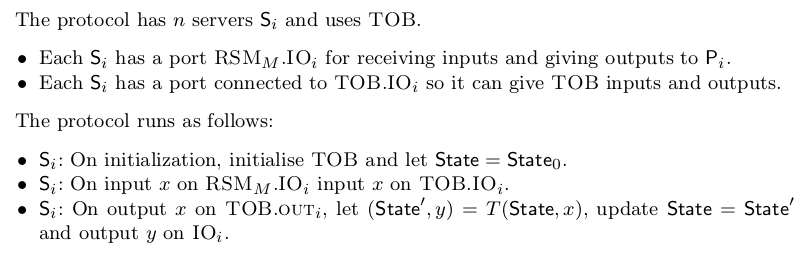
\includegraphics[width=.9\linewidth]{State Machine Replication (10)/screenshot_2018-10-21_09-02-29.png}
\end{center}

\subsection{Crypto Currencies I}
\label{sec:org33ec4c3}
\begin{itemize}
\item A popular use of state machine replications is known as \textbf{cryptocurrencies}
\begin{itemize}
\item All accounts are identified by a verification \(\text{vk}\) and the account owner has the corresponding signing key \(\text{sk}\)
\begin{itemize}
\item To spend from the account, the transaction needs to be signed by the corresponding \(\text{sk}\)
\item Ensures that only the account holder can spend any money on the account
\end{itemize}
\item It is important to use totally-ordered broadcast to be able to agree on the order in which transactions are made
\begin{itemize}
\item If there is an attempt to transfer more money from an account than it holds, the latest withdrawal has to be cancelled
\item To be able to do that all parties need to agree which transaction was the last one
\end{itemize}
\item The internal state of the machine is a list of pairs \((vk,h_{vk})\), where \(\text{vk}\) where \(vk\) is the verification key for the signature scheme and \(h_\text{vk} \in \mathbb R_0\) is the holdings of the account
\item The holdings of the initial accounts is application specific
\begin{itemize}
\item It is assumed tat some accounts \((\text{vk}, h_\text{vk})\) are build into the machine when it is created
\item The initial accounts will typically belong to the people that built the system and the ones that invested in the system
\end{itemize}
\item On input \((\text{TRANSFER}, a, \text{vk}_S, \text{vk}_R, \sigma)\), where \(a \geq 0\) and
\end{itemize}
\end{itemize}
\begin{equation}
  \text{Ver}_{\text{vk}_s}(\sigma, (\text{TRANSFER}, a, \text{vk}_R)) = \top
\end{equation}
\begin{itemize}
\item the machine will do the following:
\begin{itemize}
\item If \(a<h_{vk}_s\) then ignore the command
\item Otherwise if \((\text{vk}_R,h_{\text{vk}_s})\) exists, then retrieve it otherwise initialize it to \((\text{vk}_R,h_{\text{vk}_R} = 0)\) and update \((\text{vk}_S,h_{\text{vk}_S})\) to \((\text{vk}_S,h_{\text{vk}_S}-a)\) and update \((\text{vk}_R,h_{\text{vk}_R})\) to \((\text{vk}_R,h_{\text{vk}_R}+a)\)
\end{itemize}
\end{itemize}

\subsection{Synchronous Implementation of Totally-Ordered Broadcast}
\label{sec:org03dbd52}
\begin{itemize}
\item The following is a trivial synchronous implementation of TOP
\begin{itemize}
\item All parties broadcast their messages which ensure that all parties eventually see all the same messages
\begin{itemize}
\item Which might be in different order
\end{itemize}
\item To fix the order a leader is elected who gets to decide the order
\item The protocol blueprint is as follows:
\end{itemize}
\end{itemize}
\begin{center}
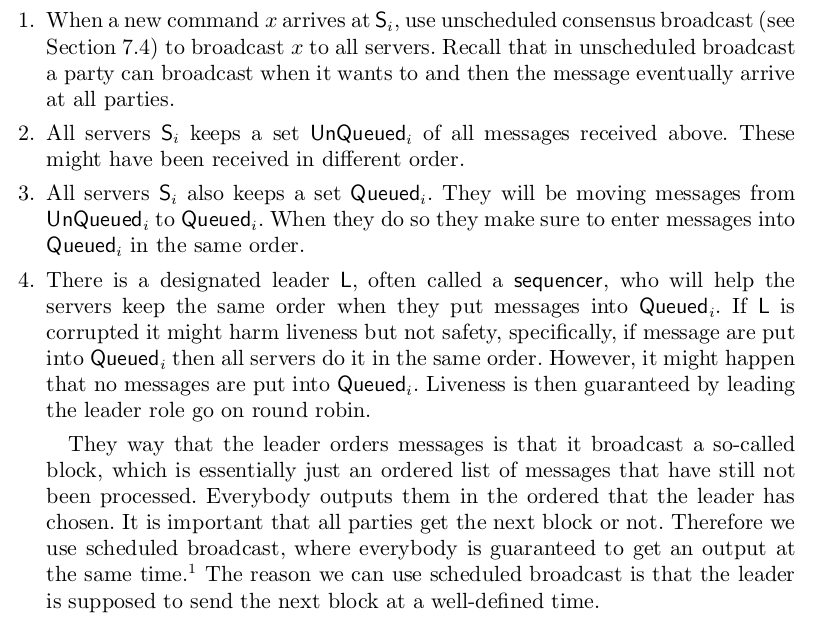
\includegraphics[width=.9\linewidth]{State Machine Replication (10)/screenshot_2018-10-21_10-28-32.png}
\end{center}

\begin{itemize}
\item Synchronous Totally-Ordered Broadcast
\end{itemize}
\begin{center}
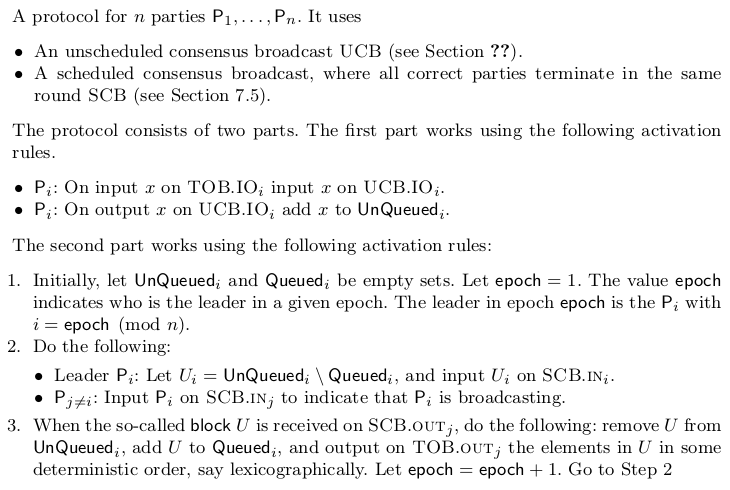
\includegraphics[width=.9\linewidth]{State Machine Replication (10)/screenshot_2018-10-21_10-36-00.png}
\end{center}

\subsection{Asynchronous Implementation of Totally-Ordered Broadcast}
\label{sec:org93f7b46}
\begin{itemize}
\item The system consists of two different parts
\begin{itemize}
\item The first on is a flooding system, which works using the following rules
\begin{itemize}
\item \(P_i:\) On input \(x\) on \(\text{TOP.IO}_i\) input \(x\) on \(\text{UCB.IO}_i\)
\item \(P_i:\) On output \(x\) on \(\text{UCB.IO}_i\) ad \(x\) to \(\text{Received}_i\)
\end{itemize}
\item The second part of the system is very different from the synchronous version
\begin{itemize}
\item The reason is that one cannot risk waiting for a particular leader
\item In each epoch all parties prose the next block and then make sure to wait until some honest parties had their block distributed to at least \(t+1\) other honest parties.
\begin{itemize}
\item We say that such block was seen by many honest
\end{itemize}
\item Each honest parties collects from \(n-t\) parties all the block that these parties have seen
\begin{itemize}
\item This means that all blocks which where seen by many honest parties will be collected by all honest parties
\end{itemize}
\item The final block will be a union of these blocks
\item To detect which block were seen by all honest parties and ensure agreement on this some Byzantine agreement is used
\end{itemize}
\end{itemize}
\end{itemize}

\begin{figure}[htbp]
\centering
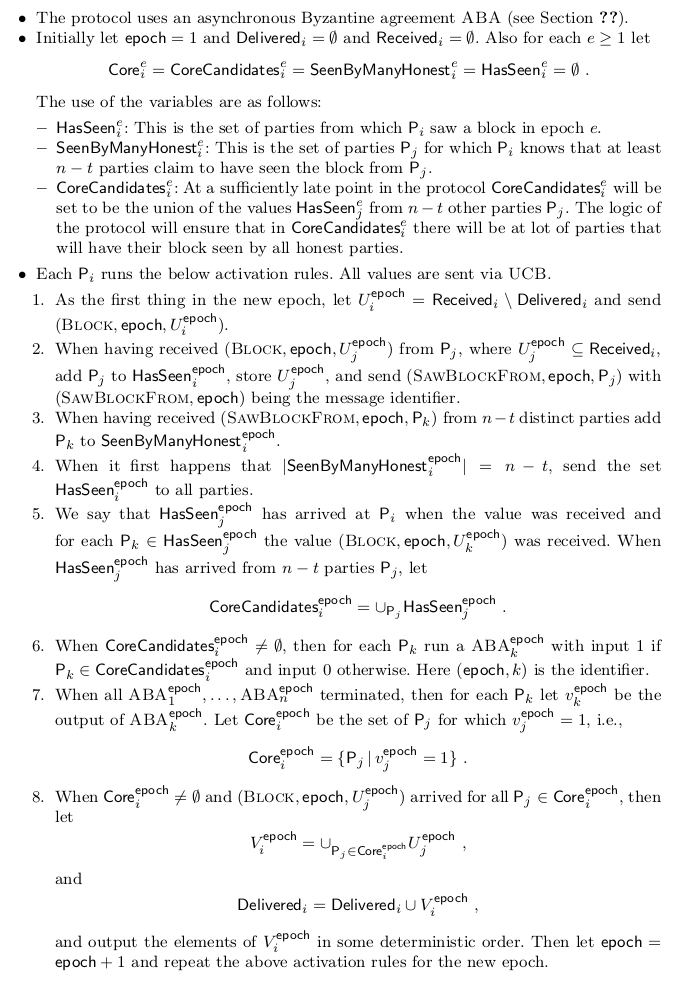
\includegraphics[width=.9\linewidth]{State Machine Replication (10)/screenshot_2018-10-21_10-51-18.png}
\caption{\label{fig:orge2c5b39}
Asynchronous Totally-Ordered Broadcast}
\end{figure}

\subsection{Group Change}
\label{sec:org269db4f}
\subsubsection{General}
\label{sec:orgaa69c54}
\begin{itemize}
\item The two protocols given assumed that the set of servers is static and that some of the servers are corrupted and some are correct
\item In practice a more realistic setting is that when some server is detected to be corrupted e.g. crashed, then it will be removed from the system and a new server will be added
\begin{itemize}
\item There might be other reasons to remove or add severs
\item Such changes are called group change
\item The challenge is to let all servers in the system agree on who is part of the system and to add and remove servers while the system is running
\end{itemize}
\end{itemize}

\subsubsection{Corruption Detection}
\label{sec:org409ff91}
\begin{itemize}
\item It is assumed that there is a subsystem \(\text{CorruptionDetection}\) which allows to detect which servers are corrupted
\begin{itemize}
\item It is a system for some servers \(\mathsf S_1, \mathsf S_2, \dots\)
\item It has the following protocols ports
\end{itemize}
\end{itemize}
\begin{center}
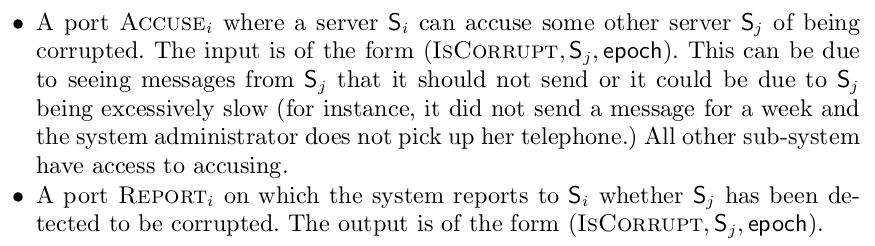
\includegraphics[width=.9\linewidth]{State Machine Replication (10)/screenshot_2018-10-21_12-00-13.png}
\end{center}
\begin{itemize}
\item We make the following requirements
\end{itemize}
\begin{center}
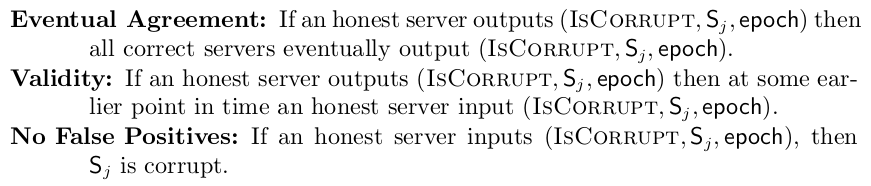
\includegraphics[width=.9\linewidth]{State Machine Replication (10)/screenshot_2018-10-21_12-00-31.png}
\end{center}

\begin{itemize}
\item The third property is a \textbf{contract property} 
\begin{itemize}
\item If you are the user of the system, then the systems promises to have all its liveness and safety properties as long as you fulfil all the contract properties.
\item The moment you break a contract property, all bets are off.
\end{itemize}

\item A way to implement this is by signing the \((\text{IsCorrupt}, S_j , \text{epoch})\) and send it along with the message
\begin{itemize}
\item If a server sees \(t+1\) correctly signed \((\text{IsCorrupt}, S_j , \text{epoch})\) for the same \(P_j\) is outputs\((\text{IsCorrupt}, S_j , \text{epoch})\)
\end{itemize}
\end{itemize}

\subsubsection{Eviction}
\label{sec:orgff9d3ec}
\begin{itemize}
\item Eviction of corrupted servers proceeds as follows
\end{itemize}
\begin{center}
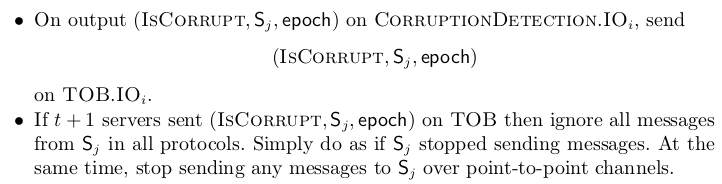
\includegraphics[width=.9\linewidth]{State Machine Replication (10)/screenshot_2018-10-21_16-52-52.png}
\end{center}

\begin{itemize}
\item The eviction procedure is secure in any system tolerating Byzantine errors
\begin{itemize}
\item A server is only evicted if it is corrupted
\end{itemize}
\end{itemize}

\subsubsection{Entry}
\label{sec:orge05bb32}
\begin{itemize}
\item To be able to add a new server and run it, the only information it needs to run the new epoch is \(\text{epoch}\), \(\text{Received}_i\) and \(\text{Delivered}_i\)
\begin{itemize}
\item This is called the entry information
\item To be able to participate it needs to get this information from somewhere
\item It can get \(\text{epoch}\) by asking the network
\begin{itemize}
\item Some servers might be slow and report an old number or no number at all
\item Other servers might be malicious ad report the wrong number
\item It is safe to adopt a too low number but not advisable to pick a too high one, since one would then do reentry from an earlier point and run a bit longer to catch up
\end{itemize}
\item If there are at most \(t\) corrupted servers, the following will do:
\end{itemize}
\end{itemize}
\begin{center}
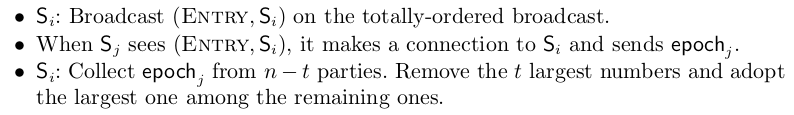
\includegraphics[width=.9\linewidth]{State Machine Replication (10)/screenshot_2018-10-21_17-07-04.png}
\end{center}

\begin{itemize}
\item The following will let \(\mathsf S_i\) learn \(\text{Delivered}\)
\end{itemize}
\begin{center}
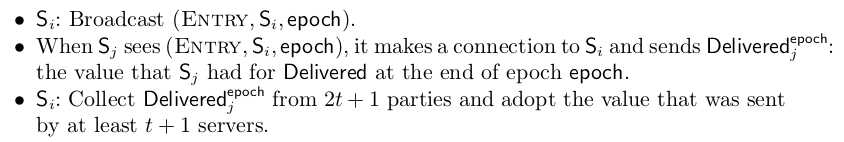
\includegraphics[width=.9\linewidth]{State Machine Replication (10)/screenshot_2018-10-21_17-08-40.png}
\end{center}
\begin{itemize}
\item Since the server \(\mathsf S_i\) knows \(\text{epoch}\) and the set \(\text{Delivered}\) at the end of the period
\begin{enumerate}
\item It sets \(\text{Delivered}_i=\text{Delivered}\)
\item Since it is perfectly possible for a server to have \(\text{Received}_i = \text{Delivered}_i\) it can now set \(\text{Received}_i = \text{Delivered}_i\)
\item It is now a fully functioning node again
\end{enumerate}

\item For at server \(\mathsf S_i\) to enter the flooding network and receive all messages that were sent in epoch \(\text{epoch}\) the following is done
\begin{enumerate}
\item Enter the flooding network to start receiving all new message
\item Ask \(2t+1\) peers to forward old messages and use majority to find the right ones
\item It adds all old and new messages to \(\text{Received}\) and starts running from state \((\text{epoch}, \text{Delivered}_i, \text{Received}_i)\)
\item It is now a fully operational new server
\end{enumerate}
\end{itemize}

\section{Blockchains (11)}
\label{sec:org01aac00}
\subsection{General}
\label{sec:org4430162}
\begin{itemize}
\item A \textbf{blockchain} is an implementation of totally ordered broadcast and can be used for anything where a totally-ordered broadcast is useful.
\item A \textbf{cryptocurrency} is a layer that can be put on top of any totally-ordered broadcast, not just the blockchain-based ones.
\end{itemize}

\subsection{Synchrony}
\label{sec:org79927d7}
\begin{itemize}
\item A notion of global physical time \(t\) is assumed
\begin{itemize}
\item Each party \(P_i\) has a local clock \(\text{Clock}_i\)
\item A bound of \(\text{MaxDrift}\) is assumed on clock drift
\begin{itemize}
\item It is assumed that \(|t-\text{Clock}_i| \leq \text{MaxDrift}/2\) for all correct \(P_i\)
\item For two correct \(P_i\) and \(P_j\) one will have the relation \(|\text{Clock}_i - \text{Clock}_j | \leq \text{MaxDrift}\)
\item It could e.g. be done by each client synchronizing against a server
\end{itemize}
\end{itemize}
\end{itemize}

\subsection{Flooding System}
\label{sec:orgf863b05}
\begin{itemize}
\item It is assumed that there is a flooding system
\begin{itemize}
\item A model is considered where parties can come and go
\item If a party is awake when a message is sent and stays awake for long enough then it is guaranteed to get the message
\item There is some fixed upper bound \(\tau\) on the delivery time
\end{itemize}

\item The ideal functionality is as follows:
\end{itemize}
\begin{center}
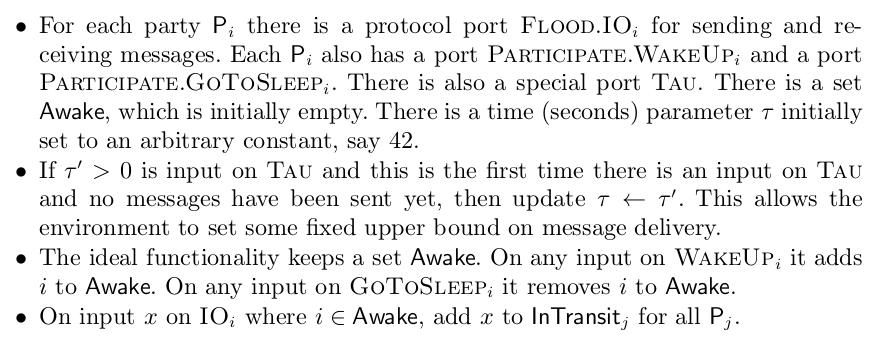
\includegraphics[width=.9\linewidth]{State Machine Replication (10)/screenshot_2018-10-28_08-26-45.png}
\end{center}
\begin{center}
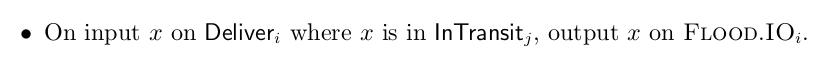
\includegraphics[width=.9\linewidth]{State Machine Replication (10)/screenshot_2018-10-28_08-26-57.png}
\end{center}


\begin{itemize}
\item For a given message \(x\)
\begin{itemize}
\item Let \(I_x\) be the time \(t\) when \(x\) was input to a correct \(P_i\) the first time
\item Let \(O_x\) be \(t\) when \(x\) was delivered at the last correct \(P_i\) that was in \(\text{Awake}\) since time \(I_c\)
\item It is assumed that \(O_x-I_x > \tau\) never happens
\item In the case where \(x\) was input to a incorrect \(P_i\) the guarantee is as follows
\begin{itemize}
\item If any correct outputs \(x\) at time \(I_x\) and \(P_i\) and \(P_j\) remains correct and alive to \(\tau\) seconds, then \(P_j\) will also output \(x\)
\end{itemize}
\end{itemize}
\end{itemize}

\subsection{Lottery System}
\label{sec:org283bcac}
\subsubsection{General}
\label{sec:orgea270f1}
\begin{itemize}
\item A lottery system \(\text{LOTTERY}\) is assumed
\begin{itemize}
\item It breaks time up into \(\text{slots}\) of length \(\text{SlotLength}\)
\item A party \(P_i\) is in slot \(\text{slot}\) if
\end{itemize}
\end{itemize}
\begin{equation}
  \text{slot}-1 \leq \frac{\text{Clock}_i}{\text{SlotLength}} < \text{slot}
\end{equation}

\begin{itemize}
\item There is a lottery system which allows a party to get a draw \(\text{Draw}_{i,\text{slot}}\) in each slot
\begin{itemize}
\item Each draw has an associated value \(\text{Val}(\text{Draw}_{i,\text{slot}})\)
\item The winner of the slot is the party with highest \(\text{Val}(\text{Draw}_{i,\text{slot}})\)
\item The lottery proceeds as follows:
\end{itemize}
\end{itemize}
\begin{center}
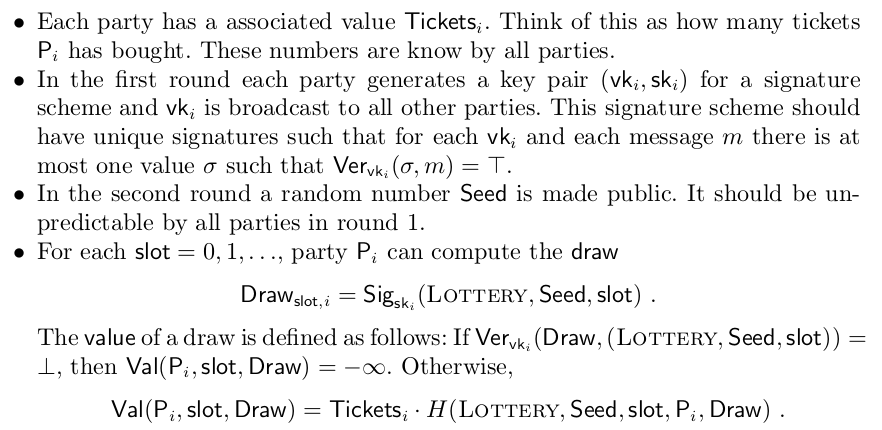
\includegraphics[width=.9\linewidth]{Blockchains/screenshot_2018-10-28_08-52-47.png}
\end{center}

\begin{itemize}
\item Since all parties know all the values \(\text{Tickets}_i\) and \(\text{vk}_i\), so all parties can compute \(\text{Val}(P_i, \text{slot}, \text{Draw}\) for all \(P_i,\text{slot}, \text{Draw}\)
\begin{itemize}
\item The reason unique signature is needed is that if \(\text{P}_i\) could compute several valid signature for \((\text{LOTTERY}, \text{Seed}, \text{slot})\), then a malicious server would get multiple attempts at winning the lottery
\begin{itemize}
\item We would like a corrupt process to lose the lottery as often as possible
\end{itemize}
\item The function \(H\) will be a cryptographic hash function with 256-bit output
\begin{itemize}
\item e.g SHA256
\end{itemize}
\item For analysis it is assumed that there is a random oracle that will output uniformly random values
\begin{itemize}
\item Except that in the same input it always outputs the same value
\item These bit strings as thought of as a number between \(0\) and \(2^{256}-1\)
\end{itemize}
\item Since the outputs of \(H\) are assumed to be uniformly random in \([0,2^{256})\) the probability that two draws will ever have the same value is negligible
\begin{itemize}
\item Each slot has a unique winner except with negligible probability
\item To be completely sure we have a unique winner, let us that if two parties \(\text{P}_i\) and \(\text{P}_j\) have \(\text{Val}(P_i,\text{slot},\text{Draw}_i) = \text{Val}(P_i,\text{slot},\text{Draw}_j)\) then we simply say that \(\text{Val}(P_i,\text{slot},\text{Draw}_i) < \text{Val}(P_i,\text{slot},\text{Draw}_j)\) when \(\text{vk}_i<\text{vk}_j\) in the lexicographic ordering
\item The short hand
\end{itemize}
\end{itemize}
\end{itemize}
\begin{equation}
  \text{Draw}_{\text{slot},i} \leftarrow \text{Draw}(\text{sk}_i, \text{slot}
\end{equation}
is used for \(\text{P}_i\) computing its draw in the slot \(\text{slot}\)  

\subsubsection{A Protocol that Almost Works}
\label{sec:org1e439f1}
\begin{itemize}
\item Assume that we have a flooding system and a lottery system
\begin{itemize}
\item We first consider a protocol where all parties participate all the time
\end{itemize}
\end{itemize}
\begin{center}
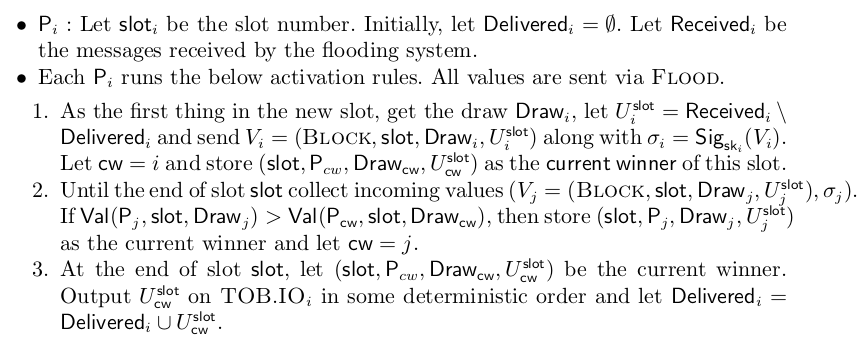
\includegraphics[width=.9\linewidth]{Blockchains/screenshot_2018-10-28_09-10-32.png}
\end{center}


\begin{itemize}
\item \textbf{Lemma 11.1} Let \(\text{MaxDrift}\) be the maximal clock drift in the network and let \(\tau\) be an upper bound on the time it takes to deliver a message. If \(\text{SlotLength} > \text{MaxDrift} + \tau\) then the following holds
\begin{itemize}
\item If \(\text{P}_\text{win}\) is honest in slot \(\text{slot}\), then all correct \(\text{P}_i\) will have \(\text{cw}_i = win\) at the end of slot \(\text{slot}\)
\item If all parties agreed on \(\text{Delivered}_i\) at the beginning of slot \$\text{slot}4, then all correct parties agree on \(\text{Delivered}_i\) at the end of slot \(\text{slot}\)
\end{itemize}

\item When \(P_\text{win}\) is correct, then \(\text{Delivered}\) grows with all the values that reached \(P_\text{win}\) before the beginning of slot \(\text{slot}\)
\begin{itemize}
\item The system is live in the sense that it does not take a message \(x\) longer to be delivered than it takes to reach all parties and then a correct process to win
\end{itemize}
\end{itemize}

\subsubsection{The Problem}
\label{sec:orgc0c911f}
\begin{itemize}
\item The problem with the protocol happens when \(\text{P}_\text{win}\) is corrupted
\begin{itemize}
\item A corrupted \(P_\text{win}\) can instead of sending \(V_\text{win}\) at the beginning of slot \(\text{slot}\) it waits until for instance \(\text{t}_\text{win}+\tau/2\)
\begin{itemize}
\item i.e. it sends it about halfway into the slot
\end{itemize}
\item As a result some parties might receive \(V_\text{win}\) and set \(\text{cw}_i = \text{win}\) and some might not have time to receive \(V_\text{win}\) and therefor set \(\text{cw}_i = \text{rup}\) where \(P_i\) is the runner up
\begin{itemize}
\item i.e. the parties with the second highest values is draw in slot \(\text{slot}\)
\item agreement is lost
\end{itemize}
\end{itemize}
\end{itemize}

\subsubsection{Creating more Problems}
\label{sec:orge44a70d}
\begin{itemize}
\item The problematic situation discussed happens where the slot winner is corrupted and sends the block late, then some correct parties might have different \(B_i=\text{BestLeft}(\text{Tree}_i)\) at the end of the slot

\item It is important for the protocol that \(\text{SlotLength}> \text{MaxDrift} + \tau\) 
\begin{itemize}
\item It turns out that the new protocol can tolerate \(\text{MaxDrift}+ \text{MaxDeliveryTime} > \text{SlotLength}\) if pnly it does not happen to often
\item It is important for efficiency as there will some variation in drift
\begin{itemize}
\item If one has to set \(\text{MaxDeliveryTime}\) such that it holds except with probability \(2^{−80}\) that the delivery time is never less than \(\text{MaxDeliveryTime}\) throughout the lifetime of the system
\item If on the other hand we have to set it such that with probability 95\% it holds then the delivery time can be set to much lower
\end{itemize}
\end{itemize}

\item An important optimization that allows to save a lot of bandwidth
\begin{itemize}
\item In the above protocol each party sends a block to each other party in each slot which creates a lot of traffic
\item A hardness threshold \(\text{Hardness}\) is introduced
\item Only parties with a ticket with value higher than \(\text{Hardness}\) will send its block
\item If we set \(\text{Hardness}\) high enough this will ensure that only a few blocks a sent to all parties in each slot
\begin{itemize}
\item Gives a dramatic optimization in bandwidth
\end{itemize}
\item As a consequence it can happen in some round that not block is send because all ticket has a value less than \(\text{Hardness}\)
\end{itemize}
\end{itemize}

\subsection{Growing a Tree}
\label{sec:orgd1af220}
\subsubsection{Protocol}
\label{sec:orgc89c091}
\begin{itemize}
\item There are two types of problems to solve
\begin{enumerate}
\item Sometimes a winning block might get delivered only to some correct parties
\begin{itemize}
\item Either because a block is sent late with malice or because the delivery time is too high in the lot
\end{itemize}
\item Sometimes there is no slot winner
\end{enumerate}

\item The solution to both of these problem is to grow a tree instead of a chain
\begin{itemize}
\item Each party is supposed to take the longest path in the tree as its chain
\item This will tend to converge on agreement
\end{itemize}

\item \textbf{Definition 11.2 (block tree)} A node is of the form \((\text{BLOCK}, \text{P}_j, \text{slot}, \text{Draw}, U,h, \sigma)\)
\begin{itemize}
\item They mean the following
\begin{itemize}
\item \(\text{BLOCK}\) just specifies the type of the tuple
\begin{itemize}
\item That it is a block
\end{itemize}
\item \(\text{slot} \in \mathbb N\) is a block number
\item \(\text{Draw}\) is the draw that was used to win the lottery
\item \(U\) is the block data
\item \(h\) is a block hash (of some previous block)
\end{itemize}
\item The value of a block \(N\) is defined to be \(\text{Val}(N.\text{P}, N.\text{slot}, N.\text{Draw})\)
\item There is a special block \((\text{BLOCK}, \bot, 0, \bot, U_0, \bot)\) with value \(\infty\) called the genesis block, where \(U_0\) is the genesis data
\begin{itemize}
\item It contains \(\text{Hadness}\) and more
\item It is sometimes just called \(G\)
\end{itemize}
\item A set \(S\) of blocks which contains \(G\) and where all blocks are valid defines a tree as follows
\begin{itemize}
\item The nodes of the tree is a subset of the nodes it \(\text{Tree}\)
\item The root of the block tree is the genesis block \(G\)
\item Edges are directed and points towards the root
\item There is an edge to \(N_1 \in \text{Tree}\) from \(N_2 \in \text{Tree}\) if and if \(N_2.h = H(N_1)\) and \(N_2.\text{slot} > N_1.\text{slot}\)
\item For a given node \(N\) we let \(\text{ParthTo}(N)\) be the list of nodes from \(G\) to \(N\) including \(G\) and \(N\) and indexet from 0
\end{itemize}
\end{itemize}

\item An important component in block chains in the notion that some path in the tree being better than other
\begin{itemize}
\item In general we just like the longest path the best
\begin{itemize}
\item This is the one we want to build on.
\end{itemize}
\item If two paths have the same length a tie breaker might want to be used
\end{itemize}

\item \textbf{Definition 11.3 (path weight)} A blockchain is a block tree where each block has at most one parent
\begin{itemize}
\item A path weight is a function \(\text{PathWeight}\) mapping blockchains in a total ordered set
\item It should have the following properties
\begin{itemize}
\item If \(P^'\) is a proper prefix of \(P\), then \(\text{PathWeight}(P^{'}) < \text{PathWeight}(P)\)
\item If \(P \ne P^'\) then \(\text{PathWeight}(P^{'}) \neq \text{PathWeight}(P)\)
\item It cannot happen that \(\text{PathWeight}(P^{'}) < \text{PathWeight}(P)\) and \(\text{Len}(\text{PathWeight}(P^{'})) > \text{Len}(\text{PathWeight}(P))\)
\end{itemize}
\item The default path weight is just the order which sort first on length of \(P\) and the \(\text{Val}(\text{Left}(P))\)
\begin{itemize}
\item So \(\text{PathWeight}(N_1) < \text{PathWeight}(N_2)\) if and only if \(\text{Len}(N_1) < \text{Len}(N_2)\) or \(\text{Len}(N_1) = \text{Len}(N_2)\) and \(\text{Val}(N_1) < \text{Val}(N_2)\)
\end{itemize}
\end{itemize}

\item \textbf{Definition 11.4 (best path, best leaf)} Let \(\text{Tree} = \text{BlockTree}(S)\) be a block tree then the best path in \(\text{Tree}\) in the path from \(G\) to a left that maximizes \(\text{PathWeight}\)
\begin{itemize}
\item We write \(P = \text{BestPath}(\text{Tree})\)
\item The best left of \(\text{Tree}\) is \(\text{BestLeaf}(\text{Tree}) = \text{Leaf}(\text{BestPath}(\text{Tree}))\)
\end{itemize}

\item The protocol uses two auxiliary functions
\begin{enumerate}
\item \texttt{GetMetaData} will ask the local system is there extra data to include in the block data
\begin{itemize}
\item Assume that \(\text{GetMetaData}(\cdot) = \emptyset\) for now
\end{itemize}
\item \texttt{ValidMetaData} will check wheter some meta data is valid
\begin{itemize}
\item Assume that \(\text{ValidMetaData}(\cdot) = \top\)
\end{itemize}
\end{enumerate}

\item The protocol proceeds as follows
\end{itemize}
\begin{center}
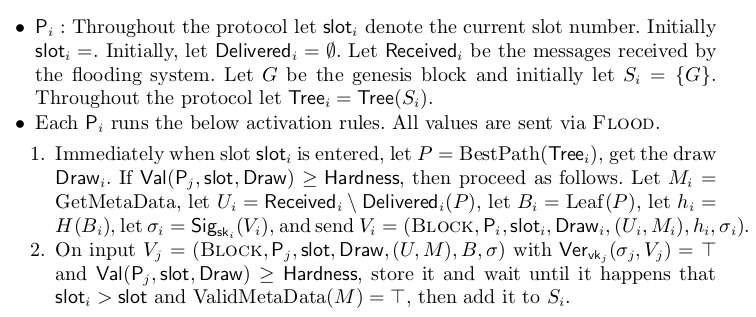
\includegraphics[width=.9\linewidth]{Blockchains/screenshot_2018-10-28_10-35-05.png}
\end{center}

\subsubsection{How does the tree grow}
\label{sec:org6d9cc2d}
\begin{figure}[htbp]
\centering
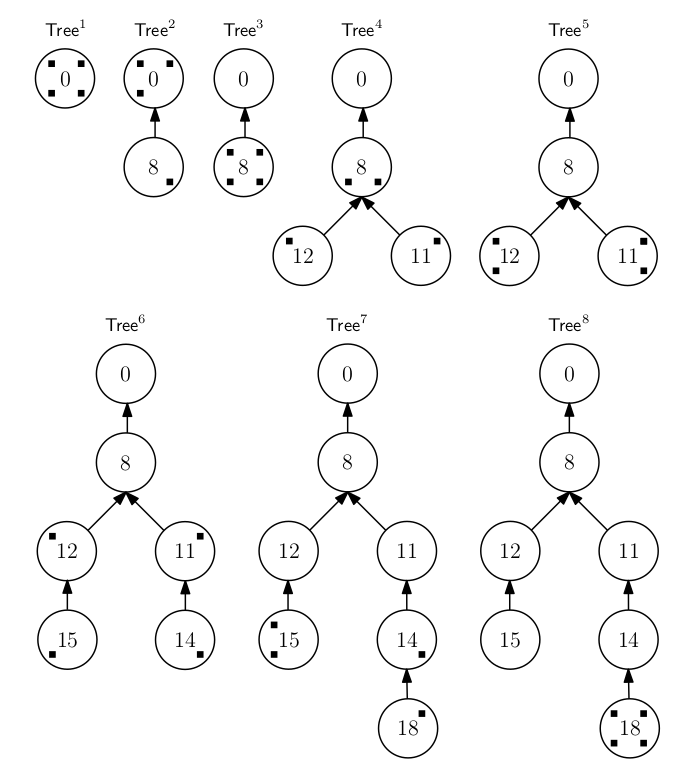
\includegraphics[width=.9\linewidth]{Blockchains/screenshot_2018-10-28_10-58-41.png}
\caption{\label{fig:orga27d636}
Example of tree growth}
\end{figure}

\begin{itemize}
\item \textbf{Definition 11.5 (honest tree)} Given two valid trees \(\text{Tree}_i\) and \(\text{Tree}_j\)  the union \(\text{Tree}_i \cup \text{Tree}_j\) is simply the tree with root \(G\) that contains all the paths of both  \(\text{Tree}_i\) and \(\text{Tree}_j\)
\begin{itemize}
\item This is again a valid tree
\item Let \(H\) be the set of all correct \(P_i\) at time \(t\) and let \(\text{Tree}_^t\) be the tree of \(P_i\) at this time
\item Let
\end{itemize}
\end{itemize}
\begin{equation}
  \text{HonestTree}^t_\text{slot} = \bigcup_{i\in H} \text{Tree}_i^t
\end{equation}
\begin{itemize}
\item By definition all correct parties at any time sees a tree which is a subset of the honest tree
\begin{itemize}
\item For all correct \(\text{P}_i\) clearly \(\text{HonestTree}^t = \text{HonestTree}^t \cup \text{Tree}^t_i\)
\item Furthermore if \(\delta_t\) is the network delivery at time \(t\) and \(P_i\) is a party which is alive at time \(t\) until time \(t+\Delta_t\) then
\end{itemize}
\end{itemize}
\begin{equation}
  \text{HonestTree}^t \subseteq \text{Tree}^{t+\delta_t}
\end{equation}
\begin{itemize}
\item as all nodes seen by any honest party at time \(t\) will reach \(P_i\) by time \(t+ \Delta_t\)
\begin{itemize}
\item If for long enough the honest tree does not grow then all honest parties will in fact see the honest tree and therefore agree on the best leaf
\item So for long enough between slot winners, all honest parties tend to build on the best path which will therefore get better and better than all small unlucky forks
\end{itemize}
\end{itemize}

\subsubsection{Rollback and Finalization}
\label{sec:org1b81965}
\begin{itemize}
\item A big problem with tree protocols is when to deliver a transaction
\begin{itemize}
\item When a party changes from a chain to another chain it is called \textbf{rollback}
\item If we want to avoid rollbacks, parties cannot deliver on \(\text{IO}_i\) any transaction that is in a branch that might later be rolled back
\item There are two different approaches to deciding when that has happened. 
\begin{enumerate}
\item A way is to just wait "long enough" and only consider a block safe when it is long enough up in the tree
\item Another approach is to run a separate process which detects which blocks are final, called a finalization layer
\end{enumerate}
\end{itemize}
\end{itemize}

\subsubsection{Ghost Growth}
\label{sec:org90d9608}
\begin{figure}[htbp]
\centering
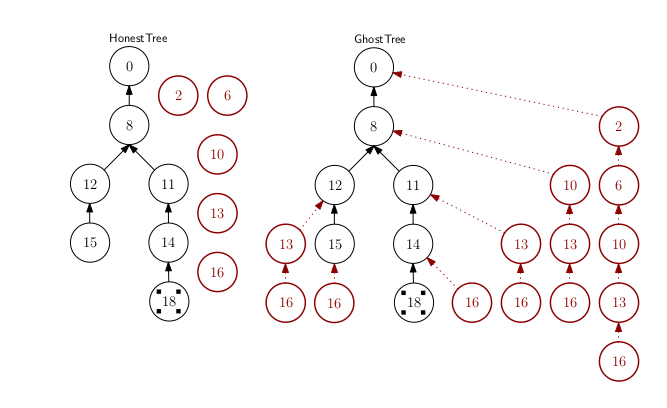
\includegraphics[width=.9\linewidth]{Blockchains/screenshot_2018-10-28_11-34-56.png}
\caption{\label{fig:org5950e74}
Example of a GhostTree}
\end{figure}

\begin{itemize}
\item To understand how far one needs to look up in the tree to find a block that will never be rolled back we need to much better how the tree grows
\begin{itemize}
\item Since winning a slot just means that \(\text{Val}(P_i),\text{slot}, \text{Draw}) \geq \text{Hardness}\) then if a corrupt party wins slot \(\text{slot}\) it can for all \(U\) and all previous block \(B\) with a small slot number produce a block \((\text{BLOCK}, P_k, \text{slot}, \text{Draw}, U, H(B), \sigma)\) which will be valid
\item A \textbf{ghost tree} is a tree that is obtained by starting with the honest tree and for each withheld winning draw, and add the corresponding blocks at all possible places
\begin{itemize}
\item In particular the corrupted parties can add a new block at any node in the ghost tree with a smaller slot number
\end{itemize}
\item The \(\text{GhostTree}\) at time \(t\) is denoted by \(\text{GhostTree}^t\)
\item By creating long ghost trees one can get long rollbacks
\item One solution which often comes to mind for limiting the problem
\begin{itemize}
\item This is a bad idea since this might result in some parties rolling back and another which do not
\end{itemize}
\end{itemize}
\end{itemize}

\subsection{Understanding Tree Growth}
\label{sec:org11ee34f}
\subsubsection{General}
\label{sec:org3c644c2}
\begin{itemize}
\item In understanding tree growth, three properties have crystallized out of the current scientific literature called
\begin{enumerate}
\item Tree growth
\item Chain quality
\item Limited rollback.
\end{enumerate}
\end{itemize}

\subsubsection{Tree Growth}
\label{sec:orgbe4e767}
\begin{itemize}
\item Tree growth basically says that the tree get higher all the time as there are more and more slot winners
\begin{itemize}
\item It is parameterized by a fraction \(\text{TreeGrowth}\) which says that about a fraction \(\text{Treegrowth}\) of the slot winner makes the tree get higher
\end{itemize}

\item \textbf{Definition 11.6 (tree growth)} Let \(\text{TreeGrowth} \in [0,1]\) be a real number
\begin{itemize}
\item We say that a protocol has a \textbf{tree growth} of \(\text{TreeGrowth}\) if after \(n\) slot winners the height of \(\text{HonestTree}\) is at least \(\text{TreeGrowth} \cdot (n-\kappa)\) except with negligible probability \(2^{-\kappa}\)
\end{itemize}

\item \textbf{Definition 11.7 (timely slot)} It is defined what it means for a slot \(\text{slot}\) to be timely
\begin{itemize}
\item Let \(t\) be the time the slot starts
\item We say slot \(\text{slot}\) is timely if all messages before time \(t-\text{MaxDeliveryTime}\) are delivered before time \(t\)
\end{itemize}

\item We call slot \(\text{slot}\) a \textbf{honest slot} if there is at least one honest winner in slot \(\text{slot}\)
\begin{itemize}
\item It might have corrupted winners too and several honest winners
\item A slot \(\text{slot}\) is called a lucky slot if it is a timely slot and a honest slot
\end{itemize}

\item \textbf{Lemma 11.8 (lucky slot)} Consider a timely slot \(\text{slot}\) and let \(\text{HonestTree}^t\) be the honest tree when the slot begins
\begin{itemize}
\item Assume that there is an honest winner in slot \(\text{slot}\)
\item Let \(\text{HonestTree}^{t-\text{MaxDeliveryTime}}\) be the honest tree \(\text{MaxDeliveryTime}\) seconds before. Then
\end{itemize}
\end{itemize}
\begin{equation}
  \text{Len}(\text{BestPath}(\text{HonestTree}^t)) \geq \text{Len}(\text{BestPath}(\text{HonestTree}^{t-\text{MaxDeliveryTime}})) + 1
\end{equation}


\begin{itemize}
\item \textbf{Definition 11.9 (wasted honest winners)} We call an honest slot winner wasted if it wins a slot which is not timely or it wins a timely slot which has another honest winner with a value of its
\begin{itemize}
\item We let \(\text{WastedHonestWinners}^t\) be the number of wasted honest slot winner at time \(t\)
\end{itemize}

\item \textbf{Theorem 11.10 tree growth} Let \(\text{HonestWinners}^t\) be the number of honest winner at time \(t\). Then
\end{itemize}
\begin{equation}
  \text{Len}(\text{BestPath}(\text{HonestTree}^t)) \geq \text{HonestWinners} ^t -\text{WastedHonestWinners}^t
\end{equation}

\begin{itemize}
\item There will be about 59\% lucky slot among the slots with a winner
\begin{itemize}
\item Means that the tree grows is 59\%
\item There will tend to be about 34\% corrupt slots
\end{itemize}
\end{itemize}

\subsubsection{Chain Quality}
\label{sec:orgb9b9189}
\begin{itemize}
\item Chain quality asks that a lot of the nodes on the best path were produced by honest parties
\begin{itemize}
\item In the extreme case where all nodes are produced by corrupted parties, they might censor some transactions by not adding them to their blocks
\item If only few nodes are produced by honest parties, the throughput of censored transactions can be lowered by the corrupted parties which can be bad enough
\end{itemize}

\item \textbf{Definition 11.11 (chain quality)} Let \(\text{ChainQuality} \in [0,1]\) be a real number
\begin{itemize}
\item We say that a protocol has a chain quality of \(\text{ChainQuality}\) if after \(n\) slot winners the best path in the best path in \(\text{HonestTree}\) has \(\text{ChainQuality} \cdot L - \kappa\) nodes that were produced by parties which were honest when they produced the node, except with negligible probability \(2^{-\kappa}\)
\item The protocol in the standard tree scenario has chain quality about 42\%
\end{itemize}
\end{itemize}

\subsubsection{Ghost Eventually Die}
\label{sec:org900298b}
\begin{itemize}
\item Ghost chain that are kept hidden for too long will eventually become much shorter than the honest tree and therefore cannot be used for a rollback
\begin{itemize}
\item Any ghost branch will eventually fall behind by \(\kappa\) nodes except with negligible probability
\end{itemize}
\end{itemize}

\subsubsection{Limited Rollback}
\label{sec:orgb0fe131}
\begin{itemize}
\item The limited rollback property ask that there is a limit \(\text{RollbackLimit}\) such that the probability that there ever are a rollback longer than this is some negligibly small probability

\item \textbf{Super slot} is defined to be one which was won by a honest party where the slot was timely and no other party either honest nor corrupt party won the slot

\item \textbf{Lemma 11.12 (super slot)} All super blocks it at different heights in the honest tree

\item All other blocks which are not super blocks are called \textbf{filler blocks}

\item \textbf{Lemma 11.13 (super slot)} Assume that a rollback is possible from branch \(B_1\) to branch \(B_2\) both rooted at node \(N\). If since \(N\) was created there were created \(s\) super blocks, then at least \(s/2\) distinct filler blocks were created

\item If one want treasonable security one should never expect to get lower than tolerating rollbacks of length 40
\end{itemize}

\subsection{How to Buy Tickets}
\label{sec:org1c28766}
\subsubsection{General}
\label{sec:org94bdb25}
\begin{itemize}
\item One approach for buying tickets that does not work is to let people make accounts as they desire and say each account has 1 tickets
\begin{itemize}
\item If there are 100 honest parties running the protocol and one corrupted party, the corrupted party could simply create 1000 fake accounts ad take over the network
\item Know as a Sybil attack
\end{itemize}
\end{itemize}

\subsubsection{Permission Blockchains}
\label{sec:org117b257}
\begin{itemize}
\item An easy solution to the buying ticks problem is to verify peoples identity when they create an account
\begin{itemize}
\item This can e.g. be done if ten big companies run a blockchain between them: they simply get to have one account each
\item The assumption on having a majority of honest tickets is then translated into an assumption that a majority of the companies are honest.
\end{itemize}
\end{itemize}

\subsubsection{Proof of Stake}
\label{sec:org57bdca8}
\begin{itemize}
\item In a fully open peer-to-peer system one cannot control who has an account in the system
\begin{itemize}
\item Anyone should be able to enter the system
\end{itemize}

\item A popular way to buying tickets when the totally-ordered broadcast is used to implement a cryptocurrency is to make the tickets proportional to the holdings of ones account
\begin{itemize}
\item The assumption is that the owner with the most money in the system are honest
\item Holders of money would have an interest in keeping the system healthy
\end{itemize}
\end{itemize}

\subsubsection{Proof of Work}
\label{sec:orgfb8e6ac}
\begin{itemize}
\item A way to fight Sybil attacks is to use \textbf{proofs of work}
\begin{itemize}
\item Sometimes called one clock-cycle, one ticket
\item Since you cannot cheat with how many clock cycles you have, they cannot be copied or freely created
\begin{itemize}
\item Build on the principles of one watt, one ticket
\end{itemize}
\end{itemize}

\item In a proof-of-work systems you typically do not win the right to fill the next slot, instead you win the right to extend the tree at a particular node
\begin{itemize}
\item To replace the \(\text{Ticket}_i\)'s place with something proportional to how much computing power one put the solution to a hard computation puzzle
\begin{itemize}
\item The harder a puzzle you can solve the more computational power you must have
\end{itemize}
\end{itemize}

\item A example of a puzzle is given a hash function \(H\), which maps into e.g. 256 bit strings find a number \(d\) such that the first \(h\) bits of \(H(d)\) is 0
\begin{itemize}
\item Since \(H\) generated random looking string the probability that the first \(h\) bits of \(H(c)\) are all \(0\) is \(2^{-h}\)
\item It can be proven that if you have an experiment which is successful with probability \(T^{-1}\) each time you repeat the times one has to repeat it is \(T\) times
\item The expected number of times one has to compute \(H\) is \(2^h\) before finding the \(d\) 
\begin{itemize}
\item Therefore presenting a number \(d\) such that \(H(d)\) has \(h\) trailing 0s is reasonable proof that you have computational power
\end{itemize}
\item It does not completely work, since a malicious party could copy an honest \(d\)
\begin{itemize}
\item To prove that you did the work, one will hash along the identity which in this case is the verification key \(\text{vk}_i\) corresponding to your secret key \(\text{sk}_i\)
\item To prove your computational power one has to find \(d\) \(H(\text{vk}_i,d)\) such that it starts with \(h\) zeroes
\end{itemize}
\item The value for ones draw is
\end{itemize}
\end{itemize}
\begin{equation}
  \text{Val}(\text{P}_i, \text{slot}, \text{draw}) = (2^{256}/H(\text{vk}_i,d)) \cdot H(\text{LOTTERY},\text{Seed}, \text{P}_i, \text{slot}, \text{Draw})
\end{equation}
\begin{itemize}
\item Since the number \(2^{256}\) is the same for all parties one might as well set
\end{itemize}
\begin{equation}
  \text{Val}(\text{P}_i, \text{slot}, \text{draw}) = H(\text{LOTTERY},\text{Seed}, \text{P}_i, \text{slot}, \text{Draw})/H(\text{vk}_i,d)
\end{equation} 
\begin{itemize}
\item \emph{Proof-of-Burning-the-Planet}: A strategy for finding \(H(\text{vk}_i, d)\) is to enter the network and start computing \(H(\text{vk}_i,c)\) for all \(c\)'s and continuously broadcasting the smallest one
\begin{itemize}
\item Would give a proof of total amount of energy spent
\end{itemize}

\item \emph{Proof-of-Hardware-Cost}: One could somehow broadcast a new seed \(\text{Seed}\) every week and then have all parties compute \(H(\text{Seed}, \text{vk}_i, c), H(\text{Seed}, \text{vk}_i, c+1) \dots\) for ten minutes and then broadcast the smallest \(H(\text{Seed},\text{vk}_i,d)\) that they found
\begin{itemize}
\item By having \(\text{Seed}\) be random and unknown until the competition starts we could ensure that no starts before
\item The machinery for mining would only be turned on for ten minutes every week
\item It would burn magnitude less energy
\end{itemize}

\item \emph{Towards Bitcoin}: Bitcoin uses the following Val for the next slot
\end{itemize}
\begin{equation}
  \text{Val} = H(\text{LOTTERY}, \text{Block}, \text{vk}_i, d)^{-1}
\end{equation}
\begin{itemize}
\item The block \(\text{Block}\) is what the miner considers as the best leaf
\begin{itemize}
\item The hash that won the lottery is added to \(\text{Block}\) in the block header
\begin{itemize}
\item The block can then at the same time function as the next seed
\item Since you are certain of a "random" output of a hash function
\end{itemize}
\item Mining goes on constantly and therefore Bitcoin is basically a \emph{Proof-of-Burning-the-Planet} system
\end{itemize}
\end{itemize}

\subsection{Finality Layers: Pruning Ghost Branches}
\label{sec:orgb451027}
\subsubsection{General}
\label{sec:org59db1d7}
\begin{itemize}
\item There will be a finalization committee \(\text{FinalityCommittee}\), which is a set of verification keys \(\text{vk}_i\)
\begin{itemize}
\item Could e.g. consists of servers that we have seen are able to stay online stably for a long time
\item Members of the committee are called the finalisers
\item Each \(\text{vk}_i\) has a number of votes, denoted by \(\text{Votes}_i\)
\begin{itemize}
\item Could e.g. be the sum of tickets of parties from the tree layer that delegated their voting power to the delegate or their number of tickets in the tree layer
\end{itemize}
\end{itemize}

\item It is important that the finalization committee is mostly honest
\begin{itemize}
\item It is assumed that at most one-third of the votes are corrupted
\item For a set \(S\) of finalisers let
\end{itemize}
\end{itemize}
\begin{equation}
  \text{Votes}_s = \sum_{i \in S} \text{Votes}_i
\end{equation}
\begin{itemize}
\item Let \(\text{Corrupt}\) be the set of the corrupted finalisers It is required that
\end{itemize}
\begin{equation}
  \text{Votes}_\text{Corrupt} < \text{Votes}_\text{FinalityCommittee}/5
\end{equation}
\begin{itemize}
\item It is assumed that we have a weak multi valued BA WMVBA
\begin{itemize}
\item It should be secure as long as \(\text{Votes}_\text{Corrupt} < \text{Votes}_\text{FinalityCommittee}/5\)
\item The following is the protocol \(\text{AGREEONBLOCK}(fid,c,h, \Delta)\) that agrees on the block at height \(h\)
\end{itemize}
\end{itemize}
\begin{center}
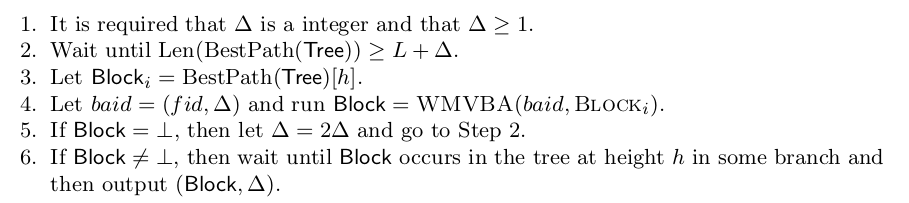
\includegraphics[width=.9\linewidth]{Blockchains/screenshot_2018-10-29_10-00-20.png}
\end{center}
\begin{itemize}
\item Input \(fid\) is a unique identifier for this run of the  protocol
\item Input \(c\) is a counter of previous finalization's
\item Input \(h\) is the height of the block to finalize
\item Input \(\Delta\) is a "delay" in when to start the finalization

\item The following is the protocol \(\text{KEEPAGREEING}(fid)\) for continuously agree on a higher and higher block:
\end{itemize}
\begin{center}
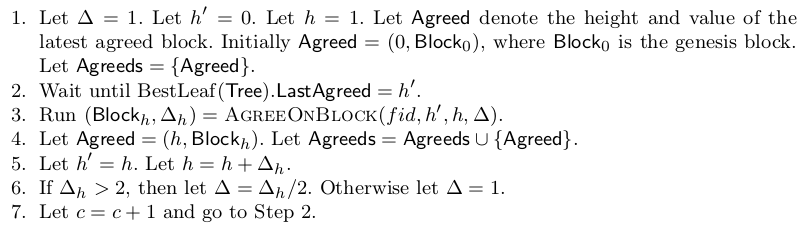
\includegraphics[width=.9\linewidth]{Blockchains (11)/screenshot_2018-10-30_19-52-31.png}
\end{center}

\subsubsection{How do We Make a Final Block Final?}
\label{sec:org9e1451a}
\begin{itemize}
\item To make sure there are no rollbacks from the blocks in \(\text{Agreed}\) the \(\text{PathWeight}\) rule is updated in such a way that makes sure they are part of the current best block

\item \textbf{Finalization Meta-Data:} When a new block \(\text{Block}\) is made the meta data \(M\) is included as a new field \(\text{LastAgreed}\)
\begin{itemize}
\item It is the maximal in the path from genesis to \(\text{Block}\) where a block from \(\text{Agreeds}\) is sitting
\item This is done via \texttt{GetMetaData()}
\item When a block \(\text{Block}\) is received it is not considered valid until \(\text{PathTo}(\text{Block}[\text{Block}.M.\text{lastAgreed}] \in \text{Agreeds}\)
\begin{itemize}
\item The  \(\text{Block}.M.\text{lastAgreed}\) should be larger that \(\text{LastAgreed}\) on all nodes in \(\text{PathTo}(\text{Block})\)

\item This check is done by \(\text{ValidMetaData}\)
\end{itemize}
\end{itemize}

\item \textbf{Prefer-Agreed-Blocks Rule}: We update the \(\text{PathWeight}\) rule such that the number of finalized blocks counts first
\begin{itemize}
\item For any \(\text{PathWeight}\) let \(\text{PathWeight}^\text{FIN}\) be the ordering which first sorts on \(\text{Block}.M.\text{LastAgreed}\) of the last block in the path and then sorts like \(\text{PathWeight}\)
\end{itemize}
\end{itemize}

\subsubsection{Pruning Ghost Branches}
\label{sec:org33267cd}
\begin{itemize}
\item Since the Ghost Branches can never be a part of the \(\text{Agreed.Block}\) it allows the ghost branches to be pruned
\begin{itemize}
\item This is due to the agreed parties being honest parties and since the ghost branch is not longer a ghost branch when it is seen by an honest party
\end{itemize}
\end{itemize}

\subsection{Dynamic Parameters}
\label{sec:org260ed67}
\subsubsection{General}
\label{sec:org3c85384}
\begin{itemize}
\item It was previously assumed that parameters like \(\text{Tickets}_i\) and \(\text{Votes}_i\) just were given
\begin{itemize}
\item When the system evolves so must the parameters
\item e.g. in a proof of state system it is important to update the \(\text{Tickets}_i\) since it is proportional to the money on the system
\item To avoid flickering when updating the parameters in can be done for instance each day
\end{itemize}
\end{itemize}

\subsubsection{BlockParameter}
\label{sec:org4ec0a2b}
\begin{itemize}
\item It turns out that it is convenient to require that dynamic parameters are a function of the parths in the tree and not a separate protocol

\item \textbf{Definition 11.14 (block parameters)} The function \(\text{BlockParameters}\) is defined which at each block in the tree specifies what are the system parameters as compute at that block
\begin{itemize}
\item Let \(\text{Block}\) be a block in \(\text{Tree}\) and \(\text{Path} = \text{PathTo}(\text{Block})\) be the path from genesis to \(\text{Block}\) in \(\text{Tree}\) then the function \(\text{BlockParameters}(\text{Tree}, \text{Block})\) is required to only be a function of \(\text{Path}\)
\begin{itemize}
\item \(\text{BlockParameters}(\text{Block})\) is written for brevity
\end{itemize}
\item At each block it returns a structure \(\text{Params} = \text{BlockParameters}(\text{Block})\) which contain the following entries:
\begin{itemize}
\item \(\text{Tickets}\) is a dictionary which for a public key \(\text{vk}\) of a baker returns the number of tickets \(\text{Tickets}[\text{vk}]\) of the baker
\item \(\text{FinalityCommittee}\)
\item \(\text{Votes}\)
\item \(\text{Hardness}\)
\item \(\text{Seed}\)
\item \(\text{SlotLength}\)
\item \(\dots\)
\end{itemize}
\item For simplicity we can imagine that there runs a special designated smart contract on the blck chain, the \textbf{parameters contract}, which computes the new parameters
\item The function \(\text{BlockParameters}\) would then just read state of this contracts
\item The \textbf{block parameters} of a block are just \(\text{BlockParameters}(\text{BLOCK})\)
\end{itemize}

\item \textbf{Definition 11.15 (slot parameters)} A function \(\text{SlotParameters}\) is defined which at each slot specifies what are the system parameters as computed at last slot
\begin{itemize}
\item It takes tree parameters \(\text{SlotParameters}(\text{Tree}, \text{Block}, \text{slot})\)
\item It is required that \(\text{Block}\) has a slot number larger or equal to \(\text{slot}\)
\item Let \(\text{Path} = \text{PathTo}(\text{Tree}, \text{Block})\) and \(\text{Block}_{\leq \text{slot}}\) be the last block in \(\text{Path}\) with a block number that is \(\leq \text{slot}\) then \(\text{SlotParameters}(\text{Tree}, \text{Block}, \text{slot}) = \text{BlockParameters}(\text{Tree}, \text{Block}_{\leq \text{slot}}\)
\begin{itemize}
\item \(\text{SlotParameters}(\text{Block}, \text{slot})\) for brevity
\end{itemize}
\end{itemize}

\item \textbf{Definition 11.16 (advance parameters)} A function \(\text{AdvanceParameters}\) is defined which at each slot specifies what are the system parameters to be used at that slot
\begin{itemize}
\item It takes tree parameters \(\text{AdvanceParameters}(\text{Tree}, \text{Block}, \text{slot})\)
\item It is required that \(\text{Block}\) has a slot number larger or equal to \(\text{slot} - \text{AdvanceTime}\)
\begin{itemize}
\item Then \(\text{AdvanceParameters}(\text{Tree}, \text{Block}, \text{slot}) = \text{SlotParameters}(\text{Tree}, \text{Block}, \text{slot} - \text{AdvanceTime})\)
\item \(\text{AdvanceParameters}(\text{Block}, \text{slot}))\) is written for brevity
\end{itemize}
\item \(\text{AdvanceTime}\) should be large
\end{itemize}

\item A new parameter is defined which is called \(\text{StableTime}\)
\begin{itemize}
\item It is how often we change the parameters
\end{itemize}
\end{itemize}
\begin{center}
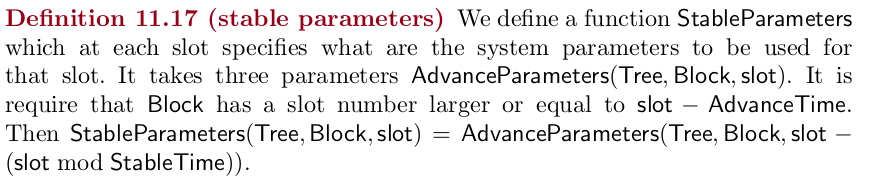
\includegraphics[width=.9\linewidth]{Blockchains (11)/screenshot_2018-10-30_21-26-39.png}
\end{center}

\begin{center}
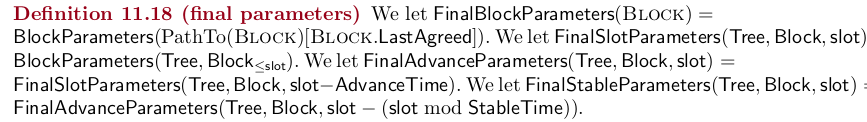
\includegraphics[width=.9\linewidth]{Blockchains (11)/screenshot_2018-10-30_21-27-22.png}
\end{center}

\begin{itemize}
\item Using final parameters of the tree layer has the advantage that you never get a rejected draw won by an honest party
\begin{itemize}
\item The disadvantage is that if finalization turns off for a long time, the distribution of not follow the movement of money in the system which might not be healthy
\item The advantage of using nonfinal parameters is on the other hand that the tickets will follow the money no matter what happens to the finalization layer.
\begin{itemize}
\item The disadvantage is that the advance time have to be set really large to reasonable account for worst case network
\item Might even a day
\end{itemize}
\item A trick that gives the best of both worlds is to use two advance times \(\text{WorstCaseAdvanceTime}\) and \(\text{FinalityAdvanceTime}\)
\begin{itemize}
\item \(\text{FinalityAdvanceTime}\) is small time which is basically the advance time we need to give the finalizers to get ready
\item \(\text{WorstCaseAdvanceTime}\) is very large
\item It uses \(\text{FinalityAdvanceTime}\) when computing \(\text{FinalAdvanceParameters}(\text{Tree}, \text{Block}, \text{slot})\)
\item It uses  \(\text{WorstCaseAdvanceTime}\) when computing \(\text{AdvanceParameters}(\text{Tree}, \text{Block}, \text{slot})\)
\end{itemize}
\end{itemize}
\end{itemize}

\subsection{Some Important Missing Details}
\label{sec:org4d8d61a}
\subsubsection{New Accounts}
\label{sec:orgcae374f}
\begin{itemize}
\item When new accounts are created the account creator could pick the secret key \(\text{sk}_i\) such that \(\text{Draw}_{\text{slot},i} = \text{Sig}_{\text{sk}_i}(\text{LOTTERY, Seed, slot})\) is higher on average than the coming slot
\begin{itemize}
\item Since the account creator knows the tree parameters it could just try several \(\text{sk}_i\) until it find a lucky one
\item To avoid this an account must use a seed published after it was created
\item A new account cannot take part in the lottery until a new seed was made
\item It is important that corrupted parties cannot influence the seed creation to much
\end{itemize}
\end{itemize}

\subsubsection{Consensus Layer Peeking}
\label{sec:org0f368b8}
\begin{itemize}
\item It is convenient to expose to the smart contract layer some value from the tree layer and the finality layer
\begin{itemize}
\item This is done via peeking contracts
\item These are contracts in the smart contract layer which contains values from the consensus layer
\item A value \(V\) can be put ion the peek contract if it is guaranteed that all honest parties agree on \(V\)
\begin{itemize}
\item They simply add it as a transaction to the next block and reject blocks that report a wrong value of \(V\)
\end{itemize}
\item An important peek is used to provide random values to the smart contact layer
\begin{itemize}
\item These random values can be used to compute \(\text{BlockParameters}(\text{Block})\)
\item Used to provide Seeds which provide fresh seeds for future lotteries
\end{itemize}
\item It can also be used to report values resulting from surveys run using Byzantine agreement
\end{itemize}
\end{itemize}

\subsubsection{Training your Blockchain}
\label{sec:org004d222}
\begin{itemize}
\item Finalization allows one to play with the parameters of your blockchain on the fly
\begin{itemize}
\item You could try to lower the Hardness to tune the blocktime, to make the blockchain run faster.
\begin{itemize}
\item If you go too low, the tree layer will start branching a lot, but the finalization layer will catch this since \(\Delta\) will grow
\end{itemize}
\item You could increase the blocktime again until the branching goes away
\begin{itemize}
\item Which will allow you to run with the lowest possible blocktime at all times.
\item In good network conditions it can be low, and when under attack it will become higher to protect the safety of the system.
\end{itemize}
\item This can all be controlled from the smart contract layer using the block parameter contract and
\end{itemize}
\end{itemize}
peek contracts

\subsubsection{The CAP Theorem}
\label{sec:org6b9e23b}
\begin{itemize}
\item A network is \textbf{partitioned} if there are two parts of it that cannot talk to each other

\item The \textbf{CAP theorem} roughly says that during a partition the system has to choose between availability and consistency
\end{itemize}

\section{Network Security Mechanisms (12)}
\label{sec:org90a725c}
\subsection{Authenticated Key Exchange}
\label{sec:orgbd781d1}
\begin{itemize}
\item Is about how to establish a secure channels based on an insecure network such as the Internet
\begin{itemize}
\item The threat model throughout that the adversary can see and modify all communication
\begin{itemize}
\item The entities being communicated with might be byzantine
\end{itemize}
\item It is assumed that two entities \(A\), \(B\) wanting to estalish a secure wanting establish a secure connection both have certificates containing public keys \(pk_A\), \(pk_B\)
\item The idea is now to use the public key pairs in some appropriate protocol to establish a short-lived session key \(K\), which is then used to provide secrecy and authentication by secret-key techniques.
\begin{itemize}
\item A motivation for this is efficiency since we do not want to encrypt large amounts of data using a slow public-key algorithm
\end{itemize}
\end{itemize}

\item An \textbf{authenticated key exchange} protocol is a protocol for two parties \(A\), \(B\)
\begin{itemize}
\item Each party starts the protocol with the intention of establishing a key with some other party
\item At the end, each party outputs either "reject", or "accept" as well as a key.
\item The protocol is said to be secure if the following three conditions hold:
\begin{itemize}
\item \textbf{Agreement:} 
\begin{itemize}
\item Assume \(A\) intends to talk to \(B\) and \(B\) intends to talk to \(A\).
\item Assume that both parties accept and \(A\) outputs key \(K_A\), while \(B\) outputs key \(KB\) Then \(KA = KB\)
\end{itemize}
\item \textbf{Secrecy} and \textbf{Authentication}: if \(A\) wants to talk to \(B\), and accepts
\begin{itemize}
\item It must be the case that \(B\) participated in the protocol and if \(B\) also accepts
\item He did indeed intend to talk to \(A\)
\item The adversary does not know the key \(K\) that \(A\) outputs
\item A symmetric condition holds for \(B\).
\end{itemize}
\item \textbf{Freshness} if \(A(B)\) follows the protocol and accepts, it is guaranteed that the key \(K\) that is output is a fresh key
\begin{itemize}
\item i.e., it has been randomly chosen for this instance of the protocol
\end{itemize}
\end{itemize}
\end{itemize}
\end{itemize}

\subsection{How to not do it}
\label{sec:org302efb9}
\begin{itemize}
\item The following is an attempt at a authenticated key exchange protocol that doesn't work
\end{itemize}
\begin{center}
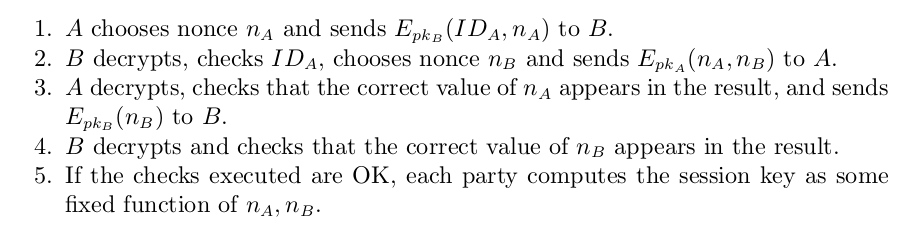
\includegraphics[width=.9\linewidth]{Network Security Mechanisms (12)/screenshot_2018-11-11_20-06-22.png}
\end{center}

\begin{itemize}
\item Example of why the protocol does not work
\end{itemize}
\begin{center}
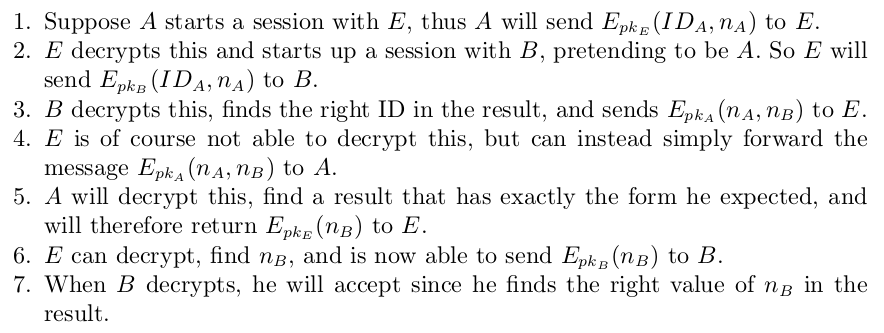
\includegraphics[width=.9\linewidth]{Network Security Mechanisms (12)/screenshot_2018-11-11_20-06-40.png}
\end{center}

\begin{itemize}
\item If there only runs one instance of the protocol there are no known attacks
\end{itemize}

\subsection{The Secure Socket Layer Protocol}
\label{sec:org658953b}
\subsubsection{General}
\label{sec:orgcb2acc4}
\begin{itemize}
\item One of most common solutions for authenticated key-exchange used today, is the \textbf{Secure Socket Layer protocol} (SSL)
\begin{itemize}
\item It uses digital signatures in addition to encryption
\item The basic idea is that one party must sign a nonce chosen by the other
\item SSL is used to set up secure http-connections on the Internet
\begin{itemize}
\item It is placed between the application and the TCP/IP transport layers
\item The data that it transports are put inside TCP/IP network packets
\item The contents of the packets can only be handled by SSL compliant clients or servers
\end{itemize}
\item It is always executed between a Server and Client
\item In its basic form, it requires that both Server and Client have public-key certificates and has the corresponding private keys.
\begin{itemize}
\item They must be able toverify each others' certificates
\end{itemize}
\item It is also possible to do a one-sided SSL where only the server has a certificate
\begin{itemize}
\item Common use case in practise
\end{itemize}
\end{itemize}

\item SSL is composed of serval protocols 
\begin{itemize}
\item \textbf{Record Protocol:} is responsible for the "raw" transmission of data
\begin{itemize}
\item Other protocols rely on this one for transporting data
\item It uses a so called \emph{cipher spec} to determine how to encrypt/decrypt and authenticate / verify data
\begin{itemize}
\item It say which encryption and other algorithms to use for thi
\item It may be empty which means no encryption should be used
\item The typical case is that encryption and authentication algorithms are specified and client and server store keys for both purposes
\end{itemize}
\item It processes a packet by
\begin{enumerate}
\item Adding a sequence number and a message authentication code to the raw data
\item This entire string is encrypted.
\item The receiver expects to receive packets in numeric order and halts if this does not happen.
\end{enumerate}
\end{itemize}
\begin{itemize}
\item This prevents replay and works because we rely on TCP/IP to make sure that packets will often arrive in the order they were sent
\end{itemize}

\item \textbf{Handshake Protocol:} is the pars of SSL that does authenticated key exchange
\begin{itemize}
\item The job of it is to bring the server and client from a state where they have an epty cipher spec and not common keys to a point where they have negotiated which algorithms to use and have done an authenticated key exchange
\item The client initially sends to the server a list of the cryptographic algorithms it supports in decreasing order of preference
\item The server then says which of the possibilities it has selected
\item Then the actual authenticated key exchange is done
\item The parties exchange Change Cipher Spec messages signal that we should now start using the negotiated algorithms and keys
\end{itemize}

\item \textbf{Change Cipher Spec Protocol}: is a one message protocol where one party tells the other to change from one cipher spec to another that has just been negotiated

\item \textbf{Alert Protocol:} is a one message protocol used to signal error messages to the other side
\end{itemize}

\item It is important to understand that even if we verify theoretically the security of the actual key exchange protocol, it does not guarantee security of the entire SSL construction.
\begin{itemize}
\item An adversary may try to manipulate messages between honest players to try to make them use an algorithm for encryption that is weaker then what they can actually use
\begin{itemize}
\item Possible since while we are doing the handshake, the communication is not yet protected.
\end{itemize}
\item Another issue is that we should of course do a Change Cipherspec just after the Handshake, so we can start using the session keys we just established.
\begin{itemize}
\item If this is not done the messages might be send in the clear
\end{itemize}
\end{itemize}
\end{itemize}
\subsubsection{The SSL key exchange}
\label{sec:org8d38cb6}

\begin{itemize}
\item This is a description of the main part of SSL, the actual key exchange protocol with many detail stripped away
\end{itemize}
\begin{center}
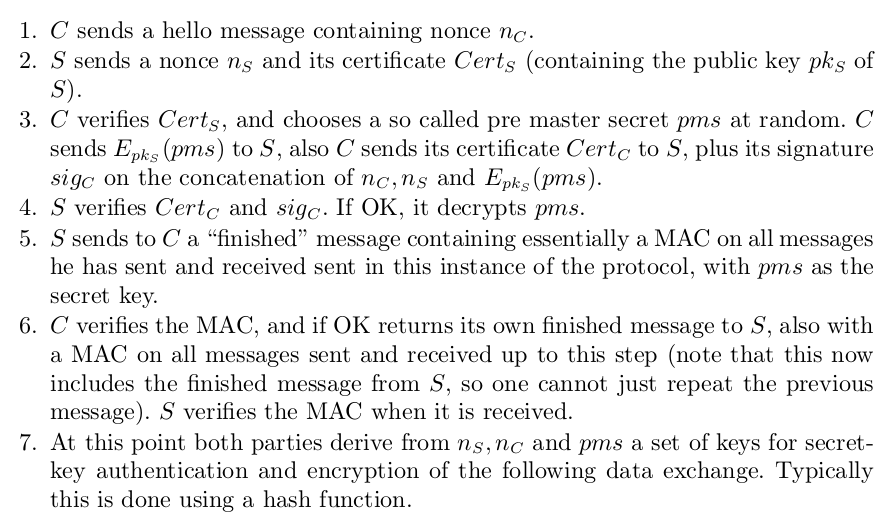
\includegraphics[width=.9\linewidth]{Network Security Mechanisms (12)/screenshot_2018-11-11_20-07-08.png}
\end{center}

\begin{itemize}
\item The idea is that \(S\) authenticates itsself by being able to send a finished message with a correct MAC
\begin{itemize}
\item This proves that it was able to compute \(pms\) and hence knows \(sk_s\)
\item The client authenticates itself by being able to sign a message containing the encryption of \(pms\)
\item \(C\) establishes that it knows the plaintext by sending a correct "finished" message at the end
\item MACing the entire view ensures that each party can check that the other party had the same view of the protocol
\begin{itemize}
\item i.e. the attacker did not change any messages
\item It forces the attacker to only look at messages sent by the peers and forward these truthfully
\end{itemize}
\end{itemize}
\end{itemize}

\subsubsection{Forward Secrecy and the Future of SSL/TLS}
\label{sec:orgd8470ea}
\begin{itemize}
\item \textbf{Forward secure} means that the security of the session cannot be comprimised even if the adversary steals a long-term secret key some time in the future
\begin{itemize}
\item A variant of the SSL handshake that is based on RSA is not forward secure
\item A variant of the SSL handshake that is based on Diffie-Hellman is forward secure
\end{itemize}
\end{itemize}

\subsection{IPSec}
\label{sec:orgbbd5572}
\subsubsection{General}
\label{sec:org8064fca}
\begin{itemize}
\item \textbf{IPSec} is a set of protocols that do a job very similar to what SSL can do, but on the transport layer
\begin{itemize}
\item It is a set of protocols for setting up a secure connection
\begin{itemize}
\item Also known as a \textbf{security association} between two ip adresses
\end{itemize}
\item Since it is on a lower layer it means that the sequence numbers and other control information are encrypted while in transit which is not the case of SSL
\item To create a security association, it uses a key exchange protocol known as the Internet Key Exchange (IKE)
\begin{itemize}
\item It is a name for a rather large set of different alternative methods.
\item Public-key certificates are used to identify the other party, just like in SSL
\item The public-key technique that is used, is known as the Diffie-Hellman key exchange
\end{itemize}
\end{itemize}
\end{itemize}

\subsubsection{(Authenticated) Diffie-Hellman Key Exchange}
\label{sec:org84fb5dd}
\begin{itemize}
\item \textbf{Diffie-Hellman key exchange} in its basic form uses
\begin{itemize}
\item A arithmetic modulo a prime number \(p\).
\item A number \(g\) in the interval from \(0\) to \(p−1\) is chosen once and for all
\item When client C and Server S want to exchange a key, we do the following:
\end{itemize}
\end{itemize}
\begin{center}
\includegraphics[width=.9\linewidth]{Network Security Mechanisms (12)/screenshot_2018-11-11_20-07-37.png}
\end{center}

\begin{itemize}
\item If \(p\) is chosen large enough, it is believed to be infeasible to compute from this information the key gab mod p.
\begin{itemize}
\item It is the so called \textbf{Diffie-Hellman problem}.
\end{itemize}

\item Issues with Diffie-Hellman key exchange
\begin{itemize}
\item Issue arise when the protocol is based on arithmetic modulo a prime
\item The problem comes from the fact that there is an algorithm known as Index Calculus that will solve the Diffie-Hellman problem, and hence break the protocol.
\item The special feature is that it will be able to do so very efficiently, if one first does a very long and inefficient preprocessing, that only depends on the prime p.
\begin{itemize}
\item It means that once the preprocessing is done for a particular prime \(p\) one can easily break any instance of the protocol that uses that prime \(p\)
\end{itemize}
\item There are several ways to solve this problem:
\begin{itemize}
\item Either a fresh new prime for the Diffie-Hellman protocol should be chosen, if not for every instance of the protocol, then at least with regular short intervals
\item A different setup can also be used, namely the Diffie-Hellman protocol can be based on so-called Elliptic Curve cryptography instead of arithmetic modulo a prime
\end{itemize}
\end{itemize}
\end{itemize}

\subsection{Comparison of SSL and IPsec}
\label{sec:orge6dcbaf}
\begin{itemize}
\item For IPsec, the communicating parties will be units with an IP number, for a standard PC or laptop, this would be the network adapter
\begin{itemize}
\item This means that the "secure tunnel" goes between such IP nodes and as soon as the network adapter delivers data to the machine it sits in, the data is no longer protected
\item All applications on the machine can use the protected connection without being aware of the encryption
\end{itemize}

\item For SSL, the communicating parties are applications, typically a browser and an Internet server
\begin{itemize}
\item This means that the applications need to know how to run SSL
\item Data are protected all the way from inside the client until it reaches the server
\item On a multiuser machine, for instance, this can be used to separate applications owned by different users.
\end{itemize}

\item Both SSL and IPSec establish secure tunnels between two entities, after the data leaves the tunnel, it is no longer protected.
\begin{itemize}
\item If what your application requires is signatures on documents, then neither SSL not IPSec are useful.
\item The situation is the same is you want to store data in encrypted form
\begin{itemize}
\item Since data are not protected when it leaves the tunel
\end{itemize}
\end{itemize}
\end{itemize}

\subsection{Password-authenticated key exchange}
\label{sec:org606e2e5}
\begin{itemize}
\item As mentioned, one flexibility offered by SSL is that one can allow for “one-way” authentication
\begin{itemize}
\item The server identifies itself towards the client but no authentication is performed of the client
\item It is the best you can do when the client does not have a certificate
\item When a secure connection is established the client can now authenticate itself by sending a password to the host over a secure connection
\begin{itemize}
\item Since the server is authenticated and the channel is encrypted, the client knows it will not be revealing the password to a malicious server.
\end{itemize}
\item The "one-way SSL plus password" method is useful, but also has some disadvantages
\begin{itemize}
\item It only allows the client to authenticate itself towards the servers it holds passwords for
\item It becomes harder to prove security of the total process because the sending of the password is not an integrated part of the protocol
\end{itemize}
\item Since guessing the password attack is an attack can never be prevented, the optimal result is to prove that this is the best possible attack.
\end{itemize}

\item \textbf{Password authenticated key exchange protocols} are relatively new, but one such protocol, known as \textbf{SRP}, has been standardized
\begin{itemize}
\item It has no security proof curerently
\item We base ourselves again on Diffie-Hellman, but with a twist, namely we encrypt the messages under the password pw that is assumed to be known by both client and server.
\item The description of the protocol below assumes a successful run where both the client and the server have the same password:
\end{itemize}
\end{itemize}
\begin{center}
\includegraphics[width=.9\linewidth]{Network Security Mechanisms (12)/screenshot_2018-11-11_20-08-08.png}
\end{center}

\begin{itemize}
\item If the passwords used by the client and the server in Step 1 are different, then the protocol will not succeed
\begin{itemize}
\item Decrypting a ciphertext with the wrong key can be typically assumed to produce just random garbage
\item The intuition for the security behind this construction is that an adversary who listens to an execution of the protocol should not be able to brute-force the password just from the transcript of the protocol
\item This protocol requires both parties to know the password in cleartext. But in most cases the server does not store the password, but instead a hash value or similar computed from the password
\begin{itemize}
\item SRP and related protocols are able to handle this case as well; they can work even if the server has some encrypted or hashed representation of the password.
\end{itemize}
\end{itemize}
\end{itemize}

\subsection{Applications of Secure Channel Set-up}
\label{sec:org52805c4}
\subsubsection{Secure http}
\label{sec:org94a5669}
\begin{itemize}
\item Secure http is simply another name for usage of SSL or TLS to set up a secure connection between a web server and a client
\begin{itemize}
\item It can be referred to directly in web addresses as \texttt{https://www....}
\item Such a connection works on a level below the application
\begin{itemize}
\item It creates a secure tunnel between the client and the server
\item Anything that goes throught is encrypted and checked for authenticity and the higher level application does not need to be aware that the connection is secure.
\end{itemize}
\end{itemize}
\end{itemize}

\subsubsection{Virtual Private Networks}
\label{sec:orgd37aa89}
\begin{itemize}
\item Virtual Private networks (VPN) solutions are designed to set up secure connections from a local area network to a remote PC.
\begin{itemize}
\item During the set-up, which happens between the PC and a VPN gateway, the remote PC is assigned an IP-address as if it was a part of the local network.
\item After setting up the connection all traffic betweenthe PC and the VPN gateway is encrypted and checked for authenticity
\item It requires, of course, that an authenticated key-exchange is done during the set-up
\item The PC can now work as if it was physically a part of the local network.
\end{itemize}
\end{itemize}

\subsubsection{Higher Level Channels}
\label{sec:org7415185}
\begin{itemize}
\item There are several protocols and solutions around that provide security for higher-level objects. For instance, the S/MIME standard
\begin{itemize}
\item MIME is the standard format in which emails are transported on the net
\item S/MIME is an extension where some extra fields are added, that allow transport of encrypted and signed emails
\item Another way to do "high-level" cryptography is the Pretty Good Privacy (PGP) software
\begin{itemize}
\item It provides capability to sign and encrypt mail and documents
\end{itemize}
\item It does not use certification of public keys by CA’s, instead it uses a concept known as "web of trust"
\begin{itemize}
\item i.e., your friends can send you a public key of a third person and assert that they trust this public key
\end{itemize}
\end{itemize}
\end{itemize}

\section{System Security Mechanisms (13)}
\label{sec:org20959d8}
\subsection{The Trusted Computing Base}
\label{sec:orgbb6531a}
\begin{itemize}
\item \textbf{System Security} is about defensive mechanism to try to prevent external attackers from getting into the system
\begin{itemize}
\item Also about preventing attacks from parties who are already users of the system
\item The typical scenario is that some party wants access to some part of our system, and we want to ensure that access is only given in cases where this is OK w.r.t our security policy
\item Getting access to a machine does not necessarily mean physical access, but could also just mean that I am allowed to communicate with it
\begin{itemize}
\item Identification is not enough it also needs to have some part that takes the decision on whether some action should be allowed according to the security policy
\item If access is denied it should not possible to circumvent the system and get access anyway
\end{itemize}
\item There needs to be a part of the system that cannot be modified by attackers
\begin{itemize}
\item It is called the \emph{trusted computing base} (TCP)
\item It can e.g. be established using hardware and/or software security depending on the threat model
\item It will often be a part of the operating system's kernel
\item It consists of one or more hardware units
\end{itemize}
\end{itemize}
\end{itemize}

\subsection{Firewalls}
\label{sec:org520d7b6}
\subsubsection{Packet Filtering}
\label{sec:org7b58403}
\begin{itemize}
\item A firewall is simply a machine or a piece of software that stops and removes part of the traffic on a network
\begin{itemize}
\item It is typically placed on the connection between a company's local network and the Internet
\item The simplest use of a firewall is to make it filter out all communication trying to connect to machines for which you do not want any communication with the outside world.
\end{itemize}

\item The simplest tool we can use in a firewall is called \emph{packet filtering}
\begin{itemize}
\item The firewall looks at each packet and decides whether the packet should be allowed through based only on the content of the packet and some fixed set of rules
\item It can e.g. remove all packets trying to open a TCP connection to a local machine and stop all UDP traffic
\item If one would have to make the firewall allow for incoming connections to e.g. the web-server or to allow users to use UDP
\begin{itemize}
\item It can be done by packet filtering, because we can determine which incoming connections is for the web-server, and which UDP packets are meant for or are coming from a known DNS server.
\item It opens up for attacks if the attacker can break into the web-server and move from there to other machines
\item It can be solved by e.g. using two firewalls
\end{itemize}

\item If simple packet filtering is to be secure, it needs to be so restrictive that it is hard to live with
\begin{itemize}
\item If we make it less restrictive, we open a possibility that an adversary can try to communicate with and attack machines on the local net
\item An attack is typically done by scanning through a large interval of IP addresses until one findsa machine that is willing to respond.
\item It is known as "port scanning"
\end{itemize}
\item The conclusion is that a firewall needs to do something more intelligent than just a simple packet filter
\begin{itemize}
\item It needs to examine packets in more detail and either take action that depends on the purpose of a packet, or even modify the packets.
\end{itemize}
\end{itemize}
\end{itemize}

\subsubsection{Proxy Firewalls}
\label{sec:orgf892af9}
\begin{itemize}
\item One radical approach to "intelligent filtering" is a \textbf{proxy firewall}
\begin{itemize}
\item It will not allow any connection at all from a local machine to the outside or vise versa
\item It will handle any connection needed on behalf of the local machines
\item If a local machine has some client software that wants to use a service on the net the client must be configured to connect to the firewall instead and then the firewall connect to the service
\item The local network is completely hidden form the outside
\begin{itemize}
\item Scanning through a large number of IP addresses will not work
\item You'll never get a response except from the firewall
\item You are forced to hack the firewall before attempting anything else
\end{itemize}
\item They are regarded highly secure
\item It is not a very flexible solution
\begin{itemize}
\item If we want to use client software for some web service on a local machine this is not possible
\item We will be forced to do some special implementation or configuration for every type of connection
\end{itemize}
\end{itemize}
\end{itemize}

\subsubsection{Stateful Firewalls}
\label{sec:orga3661ac}
\begin{itemize}
\item A \textbf{stateful firewall} keeps track of every connection going through it
\begin{itemize}
\item Whenever someone tries to open a connection it checks whether this type of connection is allowed and blocks if not
\begin{itemize}
\item There need to be some flexibility for UDP packets
\item This requires the firewall to remember which connections are active at the moment
\end{itemize}
\item It is even possible to translate the addresses used by local machines to something different in the outside traffic
\begin{itemize}
\item This hides the local addresses from an outside attacker
\item Know as a masquerading firewall
\item It makes the IP address scanning harder
\end{itemize}
\item A final step is to have the firewall inspect the behavior of a connection to see if it does something suspicious and either stop it or drop packets that have suspicious content
\begin{itemize}
\item e.g. in some attacks on web server the attacker would need to send an unusually long input string to a particular routine running on the server
\item The firewall can be configured to catch such traffic and remove it
\end{itemize}
\item The optimal configuration of the firewall of course depends on the configuration of the local network
\begin{itemize}
\item It to be updated as the structure of the local network changes
\end{itemize}
\end{itemize}
\end{itemize}

\subsection{Malicious Software and Virus Scanners}
\label{sec:org04daec8}
\begin{itemize}
\item One of the things attackers would want to do it they make it past the firewall is to install malicious software on the attacked machines. It comes in many forms
\begin{itemize}
\item \textbf{Trojan horses:} programs that appear to be useful, or goes completely unnoticed by the user,   but have some hidden malicious purpose
\begin{itemize}
\item Such as granting unauthorized access, reveal private data or destroy data
\item A well-known special case is Spyware: programs that monitor peoples’ Internet usage and send information on this to the creator of the program
\end{itemize}
\item \textbf{Viruses:} infect programs on your computer, spread themselves from one program to another, and eventually does something harmful to the machine
\item \textbf{Worms:} similar to viruses, but exist as stand-alone programs that actively try to spread themselves from one machine to the other
\end{itemize}

\item \textbf{Virus scanners} are used to find malicious software that makes it into your computer
\begin{itemize}
\item It can be used to scan all potentially dangerous files and locations on your harddisk looking for pieces of code that is known to be suspicious
\item It can use a database containing information on a large number of known viruses
\begin{itemize}
\item This is typically in the form of \textbf{virus signatures} which is particular bit patterns characteristic for particular viruses
\end{itemize}
\item They are only useful if their databases are kept up to data
\begin{itemize}
\item The largest producers of virus scanners are typically remarkably fast in updating their data files when a new virus hits the net
\item Many users do not update their own copy of the scanner, or do so too slowly
\item Infections happen because of outdated virus scanner files and not because of new viruses
\end{itemize}
\item Virus's try to fool the scanners databases by encrypting most of their code and keep a small piece of cleartext code that will decrypt the real virus
\end{itemize}

\item There are several ways an attacker can get malicious code on your machine
\begin{itemize}
\item The attacker can try to exploit weaknesses in the operating system or server software
\begin{itemize}
\item e.g. overflow attacks or similar
\item This can lead to attacks that will work if a user just visits a particular web page, provided  his operating system has some known and exploitable bug
\end{itemize}
\item In many cases it is easy to fool the user into installing the malicious code himself
\begin{itemize}
\item This is a special case of social engineering
\end{itemize}
\end{itemize}
\end{itemize}

\subsection{Intrusion Detection}
\label{sec:orgd89acaf}
\begin{itemize}
\item A different way to spot malicious software of users is to try to detect malicious behavior instead of malicious code
\begin{itemize}
\item Process and/or users are being monitored to try to detect if their behavior is suspicious
\item The advantage is that it does not depend on information on already known viruses and/or attacks
\item e.g. stateful firewalls
\end{itemize}

\item There are two approaches to deciding whether something suspicious is going on
\begin{itemize}
\item \textbf{Rule-based intrusion detection:} We set up a set of rule describing what normal behavior is
\begin{itemize}
\item Anything that is significantly different is considered illegal
\end{itemize}
\item \textbf{Statistical intrusion detection:} First gather statistics on actual honest behavior and then compare to the statistics of the observed user or program
\end{itemize}

\item The basic problem with intrusion detection is that the entity monitoring the system must be tolerant enough to allow legal behavior, but restrictive enough to catch suspicious behavior
\begin{itemize}
\item Another issue is that the entire idea is no good, if the system does not react when an attack is detected
\end{itemize}

\item A final very useful trick in the intrusion detection area is the so called \emph{"Honey-pot"} approach
\begin{itemize}
\item The idea is to create a resource on your system that will look interesting to an attacker but is actually fake
\begin{itemize}
\item A resource that no honest user would want to use
\end{itemize}
\item As a result, if activity involving the honey-pot is detected, we can assume this is adversarial activity
\item By logging such traffic one can hope, for instance, to trace it back to the attacker before he becomes aware that he is being traced
\end{itemize}
\end{itemize}

\subsection{Security Policies}
\label{sec:orgd572e45}
\subsubsection{General}
\label{sec:org0812866}
\begin{itemize}
\item \textbf{Definition 13.1} A \textbf{security policy} contains a description of the system that the policy applies to
\begin{itemize}
\item It describes the security objectives you want to achieve
\item It can take different forms
\begin{itemize}
\item It can be a specification of what different entities are allowed to do and not allowed to do
\item It can be a specification of which events we want to tolerate when the system runs
\end{itemize}
\item The system must then ensure, either that no entity can do what is not allowed, or that no event occurs that we do not want to tolerate
\begin{itemize}
\item The policy may contain a high level (non technical) description of the methods that will be used to enforce the security objectives
\end{itemize}
\item It is important to say which system we want to protect
\begin{itemize}
\item This has the purpose of limiting the problem
\item We do not have to protect something that we have explicitly defined to be outside the system
\end{itemize}
\item The security policy can be thought of as the place where we formulate the rules that the TCB should enforce.
\end{itemize}
\end{itemize}

\subsubsection{Models for Security Policies}
\label{sec:org2e2f51b}
\begin{itemize}
\item \textbf{Models for Security Policies} An abstract description of ways to design a security policy
\begin{itemize}
\item It does typically not describe a particular system
\item It often addresses particular threat models
\end{itemize}

\item \textbf{Security Policy} Is typically a realization of some model with respect to a particular concrete system
\begin{itemize}
\item It can also be based on more than one model
\item It can also not be based on any model and therefore "unique"
\end{itemize}

\item A lattice consists of a finite set \(S\) plus a relation \(\leq\). For any elements \(a,b,c \in S\) it must hold that 
\begin{itemize}
\item \(a \leq a\)
\item \(a \leq b\) and \(b \leq a\) implies \(a = b\)
\item \(a \leq b\) and \(b \leq c\) implies \(a \leq c\)
\end{itemize}

\item One may think of \(S\) as a set of different privileges or rights a user may have in a system
\begin{itemize}
\item \(a \leq b\) means that with rights \(b\), you can do at least as much as with rights \(a\)
\item It may be that some rights are not comparable
\begin{itemize}
\item Therefore the definition of a lattice does not require that the relation \(\leq\) is defined for all pair \(a,b\)
\end{itemize}
\end{itemize}

\item In order for \(S,\leq\) to be a lattice, it is required that for any \(a,b \in S\) we have
\begin{itemize}
\item There exists a \textbf{greatest lower bound} for \(a,b\)
\begin{itemize}
\item i.e. there is some \(c \in S\) such that \(c \leq a\), \(c \leq b\) and for any other \(c'\) with this property, we have \(c' \leq c\)
\end{itemize}
\item There exists a \textbf{least upper bound} for \(a,b\)
\begin{itemize}
\item i.e. some \(d \in S\) such that \(a \leq d, b \leq d\) and for any other \(d'\) with this property we have \(d \leq d'\)
\end{itemize}
\end{itemize}

\item There are (at least) to ways to use the lattice model to organize a security policy
\begin{enumerate}
\item Define \textbf{subjects} to be all users and processes in a system, which is any entity that may actively do something to other parts of the system
\begin{itemize}
\item \textbf{Objects} are resources, files, hardware devices etc.
\item We classify subjects and objects such that each of them are assigned some position in a lattice
\item A subject \(s\) with classification \(C(s)\) may do a certain operation on object \(o\) with classification \(C(o)\) if a and only \(C(s) \geq C(0)\) or is and only if \(C(s) \leq C(o)\)
\end{itemize}
\item We can assign a position in a lattice to different parts of a system
\begin{itemize}
\item We may say that information may only flow from position \(a\) to position \(b\) if \(a \leq b\)
\begin{itemize}
\item This would mean that higher positions are "more secret"
\item The policy focuses on confidentiality
\end{itemize}
\item If a policy focuses on authenticity higher positions would mean "more reliable parts of the system"
\begin{itemize}
\item We would specify that information can only flow from \(a\) to \(b\) if \(a \geq b\)
\end{itemize}
\end{itemize}
\end{enumerate}

\item The first item above gives a motivation for requiring in the definition of a lattice that least upper bounds and greatest lower bounds exist.
\begin{itemize}
\item e.g. if we have two files, classified as a, respectively b, then all users with classification least upper bound of a, b or higher can read these files
\end{itemize}

\item A model simply special case of the Lattice model is the \textbf{Bell-Lapadula model}
\begin{itemize}
\item The idea is to define a number of security levels, which are linearly ordered
\begin{itemize}
\item e.g. \(\text{public} \leq \text{secret} \leq \text{top-secret}\)
\end{itemize}
\item The model defines to rules
\begin{itemize}
\item \textbf{No read up:} Subject \(s\) may read from object \(C(s) \geq C(o)\)
\item \textbf{No write down:} Subject \(s\) may write to an object \(o\) only if \(C(s) \leq C(o)\)
\end{itemize}
\item The idea is to prevent information from flowing from higher levels to lower ones
\item It is very rigid and hard to handle in practice
\begin{itemize}
\item The system may not be able to do what it is supposed to unless some information flows downwards
\end{itemize}
\end{itemize}

\item The \textbf{Biba model} is similar to Bell-Lapadula but focuses on integrity
\begin{itemize}
\item The higher levels are the ones that contain the most reliable information
\item It has two rules
\begin{itemize}
\item \textbf{No read down:} Subject \(s\) may read from object \(o\) only if \(C(s) \leq C(o)\)
\item \textbf{No write up:} Subject \(s\) may write to object \(o\) only if \(C(s) \geq C(o)\)
\end{itemize}
\item The idea here is that information must not flow from lower levels to higher ones
\begin{itemize}
\item It ensures that highly reliable information is not "contaminated" with less reliable stuff
\end{itemize}
\end{itemize}

\item Examples of models that re not directly based on lattice structures
\begin{itemize}
\item \textbf{Chinese Wall} This is a model inspired by commercial scenarios
\begin{itemize}
\item e.g. a company \(C\) has several different clients
\item Some of these clients are competing with each other
\item A predefined predicate \emph{compete} is assumed
\begin{itemize}
\item \(compete(c_1,c_2)\) for clients \(c_1\) and \(c_2\) is true if and only if \(c_1,c_2\) are competitors
\end{itemize}
\item The rule is that subject \(s\) is granted access to information about \(c\) if and only if he never accessed information on any \(c'\) for which \(compete(c, c')\) is true
\begin{itemize}
\item This rule is dynamic since as soon as \(s\) has accessed information on \(c\) this prevents him from accessing information from any competitor of \(c\)
\end{itemize}
\end{itemize}
\item \textbf{Prevent-Detect-Recover} The idea is to split the policy in 3 parts
\begin{itemize}
\item One part describing how we will try to prevent attacks from happening at all
\item A part describing how we can detect a successful attack
\item A part describing how we will recover once we detected a breach of security
\end{itemize}
\item \textbf{Separation of Duty} is a model that comes in two flavors:
\begin{itemize}
\item \textbf{Dual Control} is a model where certain action are defined to be possible only if they have been authorized by several persons or entities
\begin{itemize}
\item A well known example is the use of nuclear weapons
\end{itemize}
\item \textbf{Functional Separation} is a model where an action requires involvement of several persons or systems, but at different points in time
\begin{itemize}
\item e.g. signing up for an exam
\end{itemize}
\end{itemize}
\end{itemize}
\end{itemize}

\subsection{Access Control}
\label{sec:orgeb170cc}
\subsubsection{General}
\label{sec:orgf9ad0ec}
\begin{itemize}
\item It is implicitly assumed that when a users wants to execute an operation on some object able to verify the identity of the user and figure out which rights and privileges he has
\begin{itemize}
\item Checking the identity of the users and figuring out which rights and privileges he has is a technical problem
\item Figuring out which rights the user has is a different problem
\begin{itemize}
\item In principle, this can be computed from the ’s identity and the security policy
\item Doing so on the fly while a user is waiting for access, for instance requires that the information about this is organized in a appropriate way
\end{itemize}
\end{itemize}

\item The generic way to represent the information is known as the \textbf{Access control matrix}
\begin{itemize}
\item It is a matrix \(A\) with a row for each subject \(s\) and a column for each object \(0\)
\item Entry \(A[s,o]\) contains a list of all operations \(s\) is allowed to execute on \(o\)
\item On realistic systems storing the entire matrix in a central location is not practical
\end{itemize}

\item In practice two basically different approaches are taken
\begin{itemize}
\item \textbf{Access Control Lists} Here we store, together with each object the column assigned to the object
\begin{itemize}
\item This is called an access control list (ACL)
\item Such list make it easy to decide for a given object who has access
\item It is much harder to say what a given subject can do
\item This is basically the approach of the UNIX system
\end{itemize}
\item \textbf{User Capabilities} Here we store subject, the row assigned to the subject
\begin{itemize}
\item This is called a user capability
\item They make it easy to compute what a given user can do
\item It makes it harder to decide who has access to a given object
\item Windows uses this basic approach
\end{itemize}
\end{itemize}

\item For large systems, ACL's gets too long if they are specified per subject
\begin{itemize}
\item One typically splits subjects into predefined groups
\item The ACL says only what subjects from each group can do
\item UNIX splits subjects from the point of view of a single user, into: the user himself, the user group he is in, and anyone else
\begin{itemize}
\item Groups also make it possible for several subjects to share the same list of user capabilities
\end{itemize}
\item A variant of the user group idea is known as \textbf{role-based access control}
\begin{itemize}
\item A number of roles are defined, such as "ordinary user", administrator", etc. and the capabilities are specified for each role
\item Users are assigned a certain role when they log in and are granted access according to the role
\end{itemize}
\end{itemize}
\end{itemize}

\subsubsection{When the Access Control Matrix is Dynamic}
\label{sec:orgda7a38a}
\begin{itemize}
\item There are basically two approaches for updating the access control matrix \emph{mandatory access control}, where subjects cannot change the matrix, and \emph{discretionary access control} where subjects have the power to update the matrix, or parts of it
\begin{itemize}
\item Given that access control matrix may change over time it is natural to ask what types of information flow this may allow
\item e.g. can a certain access right \(r\) ever be added to some cell \(A[s, o]\) that did not contain \(r\) before
\item Harrison, Ruzzo and Ullman have studied this question in a formal model, where certain primitive operations on access control matrix A are allowed, namely
\begin{itemize}
\item Create/delete subject \(s\)
\item Create/delete object \(o\)
\item Add/delete access right \(r\) from \(A[s, o]\)
\end{itemize}
\item It is assumed that there is a fixed finite number of different access rights
\item A command has the following format:
\end{itemize}
\end{itemize}
\begin{verbatim}
Command com(parameter-list)
r1 is in A[s1,o1]
..
rn is in A[sn,on]
list of primitive operations
\end{verbatim}
\begin{itemize}
\item The meaning is that the list of primitive operations will be executed if all the conditions in the first part are satisfied
\begin{itemize}
\item All the rights, subjects and objects referred to in the specification of \texttt{com} are taken from the parameter list
\item If one is given a fixed set of commands \(com_1, \dots, com_t\) and an initial access control matrix one can ask for given access right \(r\), does there exist a set of commands that will transform \(A\) into a matrix \(A'\), where \(r \in A'[s, o]\) for some \(s,o\) but where \(r \notin A[s, o]\)
\begin{itemize}
\item If the answer is no \(A\) is safe with respect to \(r\)
\end{itemize}
\item One may want to prove
\begin{itemize}
\item If commands may contain more than one operation, then it is undecidable whether \(A\) is safe w.r.t. \(r\).
\item If all commands only contain a single primitive operation, then it is decidable whether \(A\) is safe w.r.t. \(r\).
\item If there is a upper bound fixed ahead of time on the number of subjects and objects, then it is decidable if \(A\) is safe w.r.t. \(r\).
\end{itemize}
\end{itemize}

\item Therefore the conclusion is that when designing dynamic access control sys tems, the best advice is: keep it simple!
\end{itemize}

\section{Attacks and Pitfalls (14)}
\label{sec:org0d89e3e}
\subsection{Categorizing Attacks}
\label{sec:org2081f04}
\subsubsection{General}
\label{sec:org759b881}
\begin{itemize}
\item A way to characterize what a attack based on what the attacker is trying to achieve (\textbf{STRIDE})
\begin{itemize}
\item \textbf{Spoofing Identity}: results the attacker being able to impersonate another person (user)
\item \textbf{Tampering}: results in attacker being able to manipulate data without being detected
\item \textbf{Repudiation}: results in the attacker being able to deny doing something he actually did
\item \textbf{Information Disclosure}: results in the attacker being able to access data he should not see
\item \textbf{Denial of service}: results in the attacker being able to deny others access to a system
\item \textbf{Elevation of privilege}: results in the attacker being able to have more rights that he should have
\end{itemize}

\item The same attack might have several different effects at the same time
\begin{itemize}
\item Depends on the context
\end{itemize}
\end{itemize}

\subsubsection{What means are used in the attack: X.800}
\label{sec:org8559695}
\begin{itemize}
\item A way to characterize attackers are according to the means utilized by the attacker
\item The X.800 standard operates with two main types of attacks on network transmission
\begin{itemize}
\item \textbf{Passive Attacks:}
\begin{itemize}
\item \textbf{Eavesdropping:} The attacker listens in and looks at the information sent
\item \textbf{Traffic Analysis:} The attacker only looks at who is sending to who and how much is sent
\end{itemize}
\item \textbf{Active Attacks:}
\begin{itemize}
\item \textbf{Replay:} The attacker resends an old message
\item \textbf{Blocking:} The attacker stops a message from arriving
\item \textbf{Modification:} The attacker changes the data sent or injects a new message of his own
\end{itemize}
\end{itemize}

\item Passive attacks are very difficult to detect
\begin{itemize}
\item A defense it to use encryption against eavesdropping
\item Encryption cannot stop traffic analysis
\item Ways to avoid traffic analysis
\begin{itemize}
\item Send the same message to many parties to hide intended receiver
\item Randomize the length of the message to hide the size of the actual message
\end{itemize}
\item A message known as stenography can be used to hide information inside a message
\begin{itemize}
\item e.g. make slight changes to a digital picture to hide a message
\end{itemize}
\end{itemize}

\item Active attacks are easier to detect
\begin{itemize}
\item The focus on detection of attacks, using MACs, signatures, sequence number of message etc.
\end{itemize}
\end{itemize}

\subsubsection{Where are we attacked, an by whom: EINOO}
\label{sec:orgf74089b}
\begin{itemize}
\item \textbf{Who} attacks us
\begin{itemize}
\item \textbf{External attackers:} who are not legal users of the system
\item \textbf{Insiders:} Who are registered as users of our system and so have some amount of access to start with
\end{itemize}

\item \textbf{Where} the attacker is able to hit us
\begin{itemize}
\item \textbf{Network attacks:}
\begin{itemize}
\item The adversary can only listen and perhaps modify network traffic
\item Limited to the means described in X.800
\item It is usually impossible to prevent that network attacks are attempted but most of them can be defended against against using cryptography
\end{itemize}
\item \textbf{Off-line attacks:}
\begin{itemize}
\item The adversary gets unauthorized access to information that is stored permanently in the system
\item He can steal and/or modify the information
\item Such as stealing the password database file
\item Harder than network since they require to break the systems access control
\item Cryptographic protection of data is a obvious defense against off-line attacks
\begin{itemize}
\item Since the keys has to be stored somewhere an if the adversary has access to this, this protection is then useless
\end{itemize}
\end{itemize}
\item \textbf{On-line attack:}
\begin{itemize}
\item The adversary breaks into the system while programs handing sensitive information are running
\item He may be able to read secret keys from RAM
\item They are harder to mount than off-line
\item The adversary needs to completely break the systems access control
\item They can have very severe consequences and can only be defended against by having different parts of the system protected in different ways
\end{itemize}
\end{itemize}

\item The EINOO classification can be useful when designing threat models for concrete systems
\end{itemize}

\subsubsection{Where did we make the mistake: TPM}
\label{sec:orgb13b271}
\begin{itemize}
\item A final way to categorize attacks is according to what makes the attack possible
\begin{itemize}
\item \textbf{Threat model:} The attack is possible because the thread model was not complete
\begin{itemize}
\item An attack not thought about turned out to be relevant
\end{itemize}
\item \textbf{Policy:} The attack is possible because the specification of the security policy expresses something different from what we intended
\item \textbf{Mechanism:} The attack is possible because the security mechanisms can be circumvented
\end{itemize}
\end{itemize}

\subsection{Examples of Attacks}
\label{sec:org50c2e41}
\subsubsection{Illegal Inputs}
\label{sec:orgda6e5c3}
\begin{itemize}
\item The most important type of attack in practice is the type that circumvents security mechanisms by exploiting mistakes in the software that supposedly implements the mechanisms.
\begin{itemize}
\item It takes a number of different forms
\item The attacker gives some input to the program where the input has a form that the programmer did not expects
\item It may cause the program to behave in some inappropriate way that the attacker may be able to explid
\item Usually happens when the data is interpreted as something else than just data
\end{itemize}

\item In an \textbf{overflow attack} the adversary gives input to a program that is longer than expected
\begin{itemize}
\item If the programmer did not check for this properly some bad things can happen
\item Programs written in C may have this problem
\item C does not have any built-in protection against many kinds of run-time errors such as writing outside an array
\end{itemize}

\item \textbf{The Unicode Exploit}
\begin{itemize}
\item The IIS is supposed to check whether the requests it gets from outside try to access dictionaries that should not be accessed
\item Requests are allowed to contain unicode characters
\begin{itemize}
\item This allows directory names to contain all kinds of international characters
\item They must be decoded before taking action
\end{itemize}
\item The IIS previously did the security check before the decoding
\begin{itemize}
\item This allows the attacker to mask an offending request by encoding it in unicode in a special way that the security check will not recognize
\item The attack consists of sending carefully masked request to the ISS
\item This would run with same rights as the IIS
\item The attacker can upload an run various interesting software to the target computer
\end{itemize}
\end{itemize}

\item In \textbf{Cross-Site Scripting}, the attacker exploits poor design of web pages
\begin{itemize}
\item A web site might be vulnerable to cross-site scripting if it has a page that accepts input from a client and then echoes this input back to the user in a new page
\item It is possible to fill in the search block with executable JavaScript code
\begin{itemize}
\item When the string comes back the browser will execute this code
\item This can be used to fool other users of the system
\end{itemize}
\end{itemize}

\item \textbf{The Heart Bleed Bug}
\begin{itemize}
\item Occurred in OpenSSL which is an open-source software package that implements SSL/TLS
\item The client can confirm that the server still is alive
\begin{itemize}
\item This is done by sending a nonce to the server and have the server return the same nonce
\item The client sends both the nonce and its length
\end{itemize}
\item The server has at some point store in RAM both the nonce and the length \(\ell\)
\begin{itemize}
\item It will produce the message to the client by reading \(\ell\) characters from the array
\end{itemize}
\item The Heart Bleed bug was a simple case of missing input validation
\item If a malicious client sends a length that is much too large, the server will continue to read beyond the end of the array and will return some piece of its internal memory to the client
\end{itemize}
\end{itemize}
\end{document}